\chapter{Results}%
\label{ch:results}
In this chapter the results of the \VHbb\ multi-variate discriminant fit are
shown. Other results such as those for the cross-checks of the analysis can be
found in~\cite{VHMainNote2019}. As my contributions were significant in the
modelling of backgrounds and the study of the profile-likelihood fit the
nuisance parameter pulls are included in this chapter. My contributions to the
results are as already stated in other chapters plus running the combined, and
2--lepton channel fits to generate and study the results at many key milestones
in the publication timeline including the final results in the
paper~\cite{final-paper}.

\section{Nuisance Parameter Pulls}
% Describe anything in the pulls and correlations that is particularly relevant to
% the parts of the analysis that I worked on, V + jets systematics in particular.

% Omit pulls of little significance referring to the internal note.

% (+ add in chapter 6 brief description of the treatment of systematics in the
% fit, i.e. what do we prune, state that there is smoothing and cite)
Figures~\ref{fig:nppulls_012L_MVAVH_a} and \ref{fig:nppulls_012L_MVAVH_b} show a
subset of the nuisance parameter pulls and free parameter scale factors in the
profile-likelihood fit.
% \begin{figure}[hb]
% \centering
% 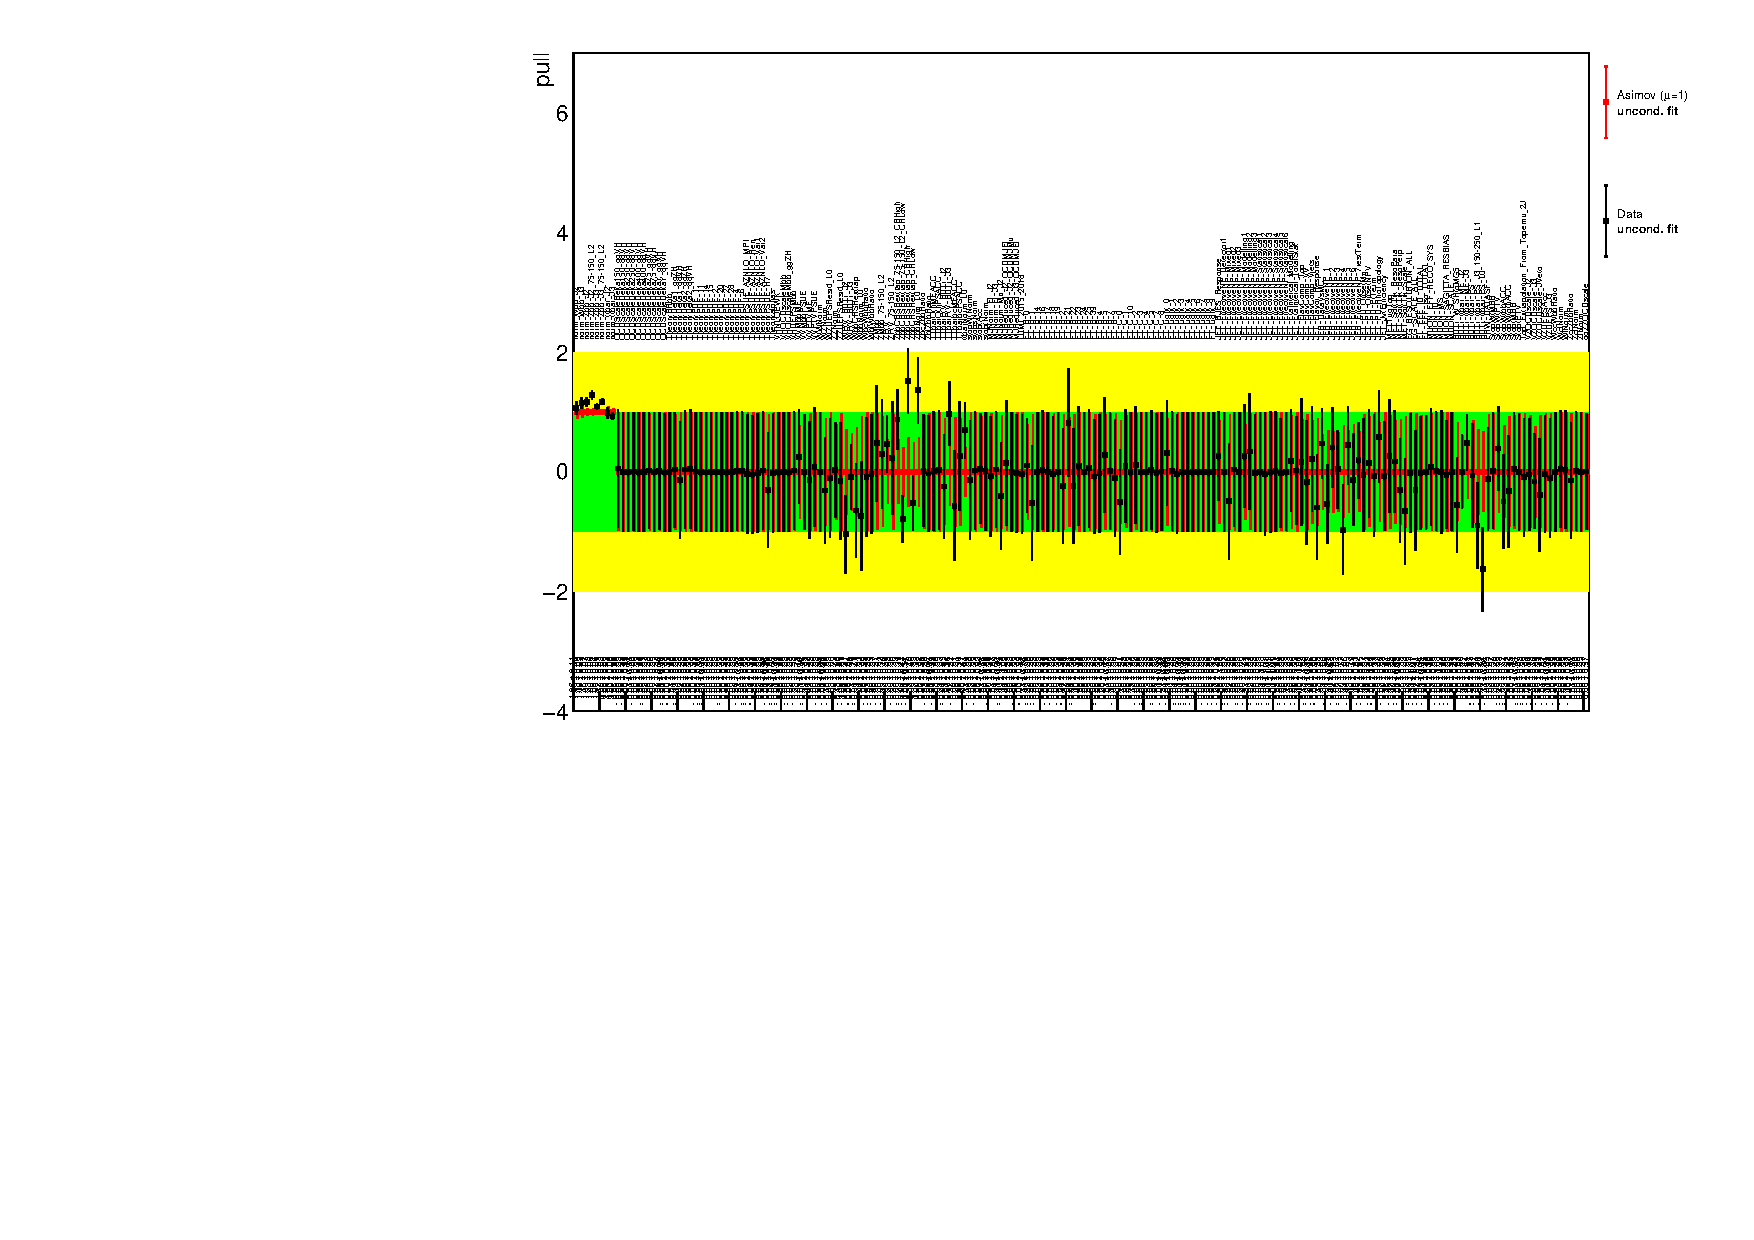
\includegraphics[angle=270]{final_fit_mva/pullComparisons/NP_allExceptGammas.pdf}
% \caption{caption}
% % Nuisance parameter pulls and the free parameter scale factors corresponding to
% % an unconditional combined fit performed to the Asimov dataset (red) and an
% % unconditional combined fit to the \RunTwo data (black).
% \label{fig:nppulls_012L_MVAVH} 
% \end{figure}
%
\begin{figure}[hb]
\centering
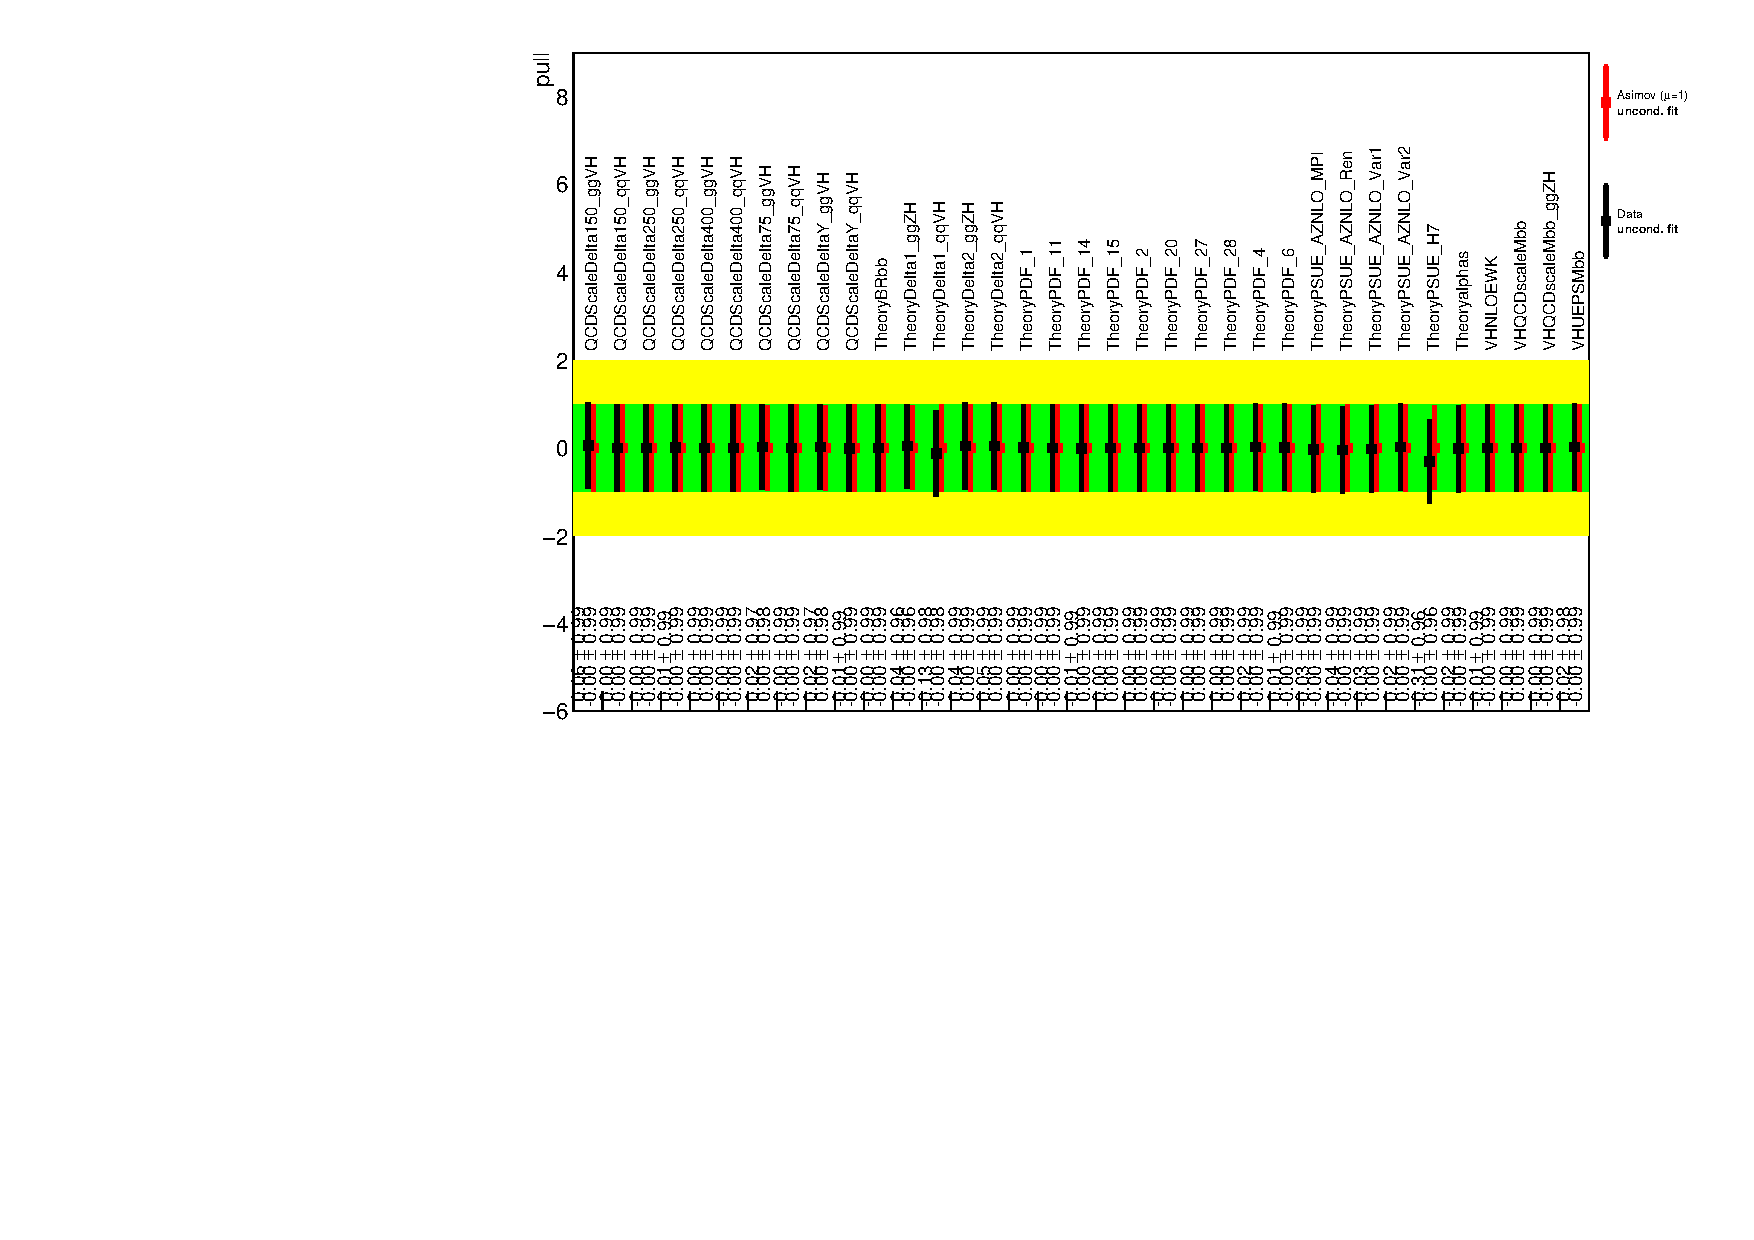
\includegraphics[width=0.49\linewidth]{final_fit_mva/pullComparisons/NP_VH.pdf}
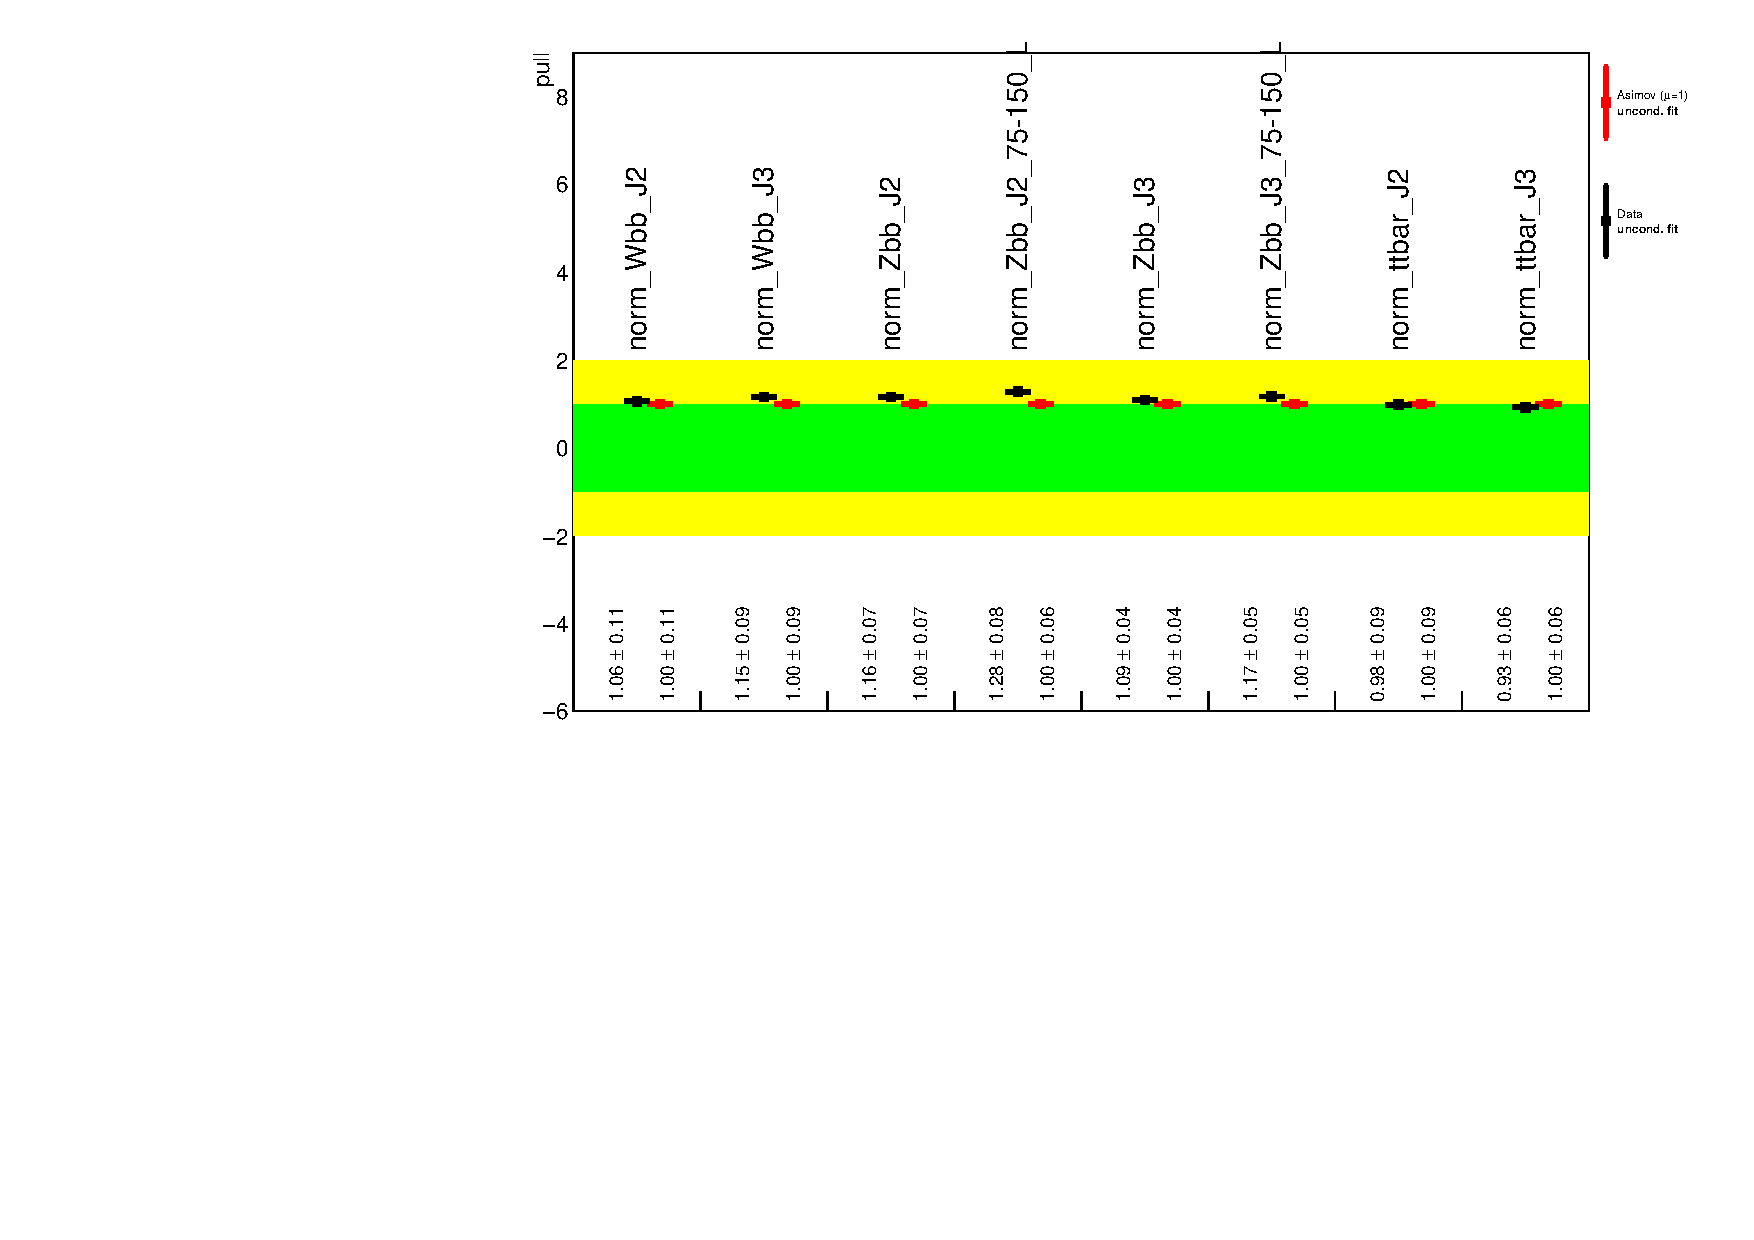
\includegraphics[width=0.49\linewidth]{final_fit_mva/pullComparisons/NP_FloatNorm.pdf}
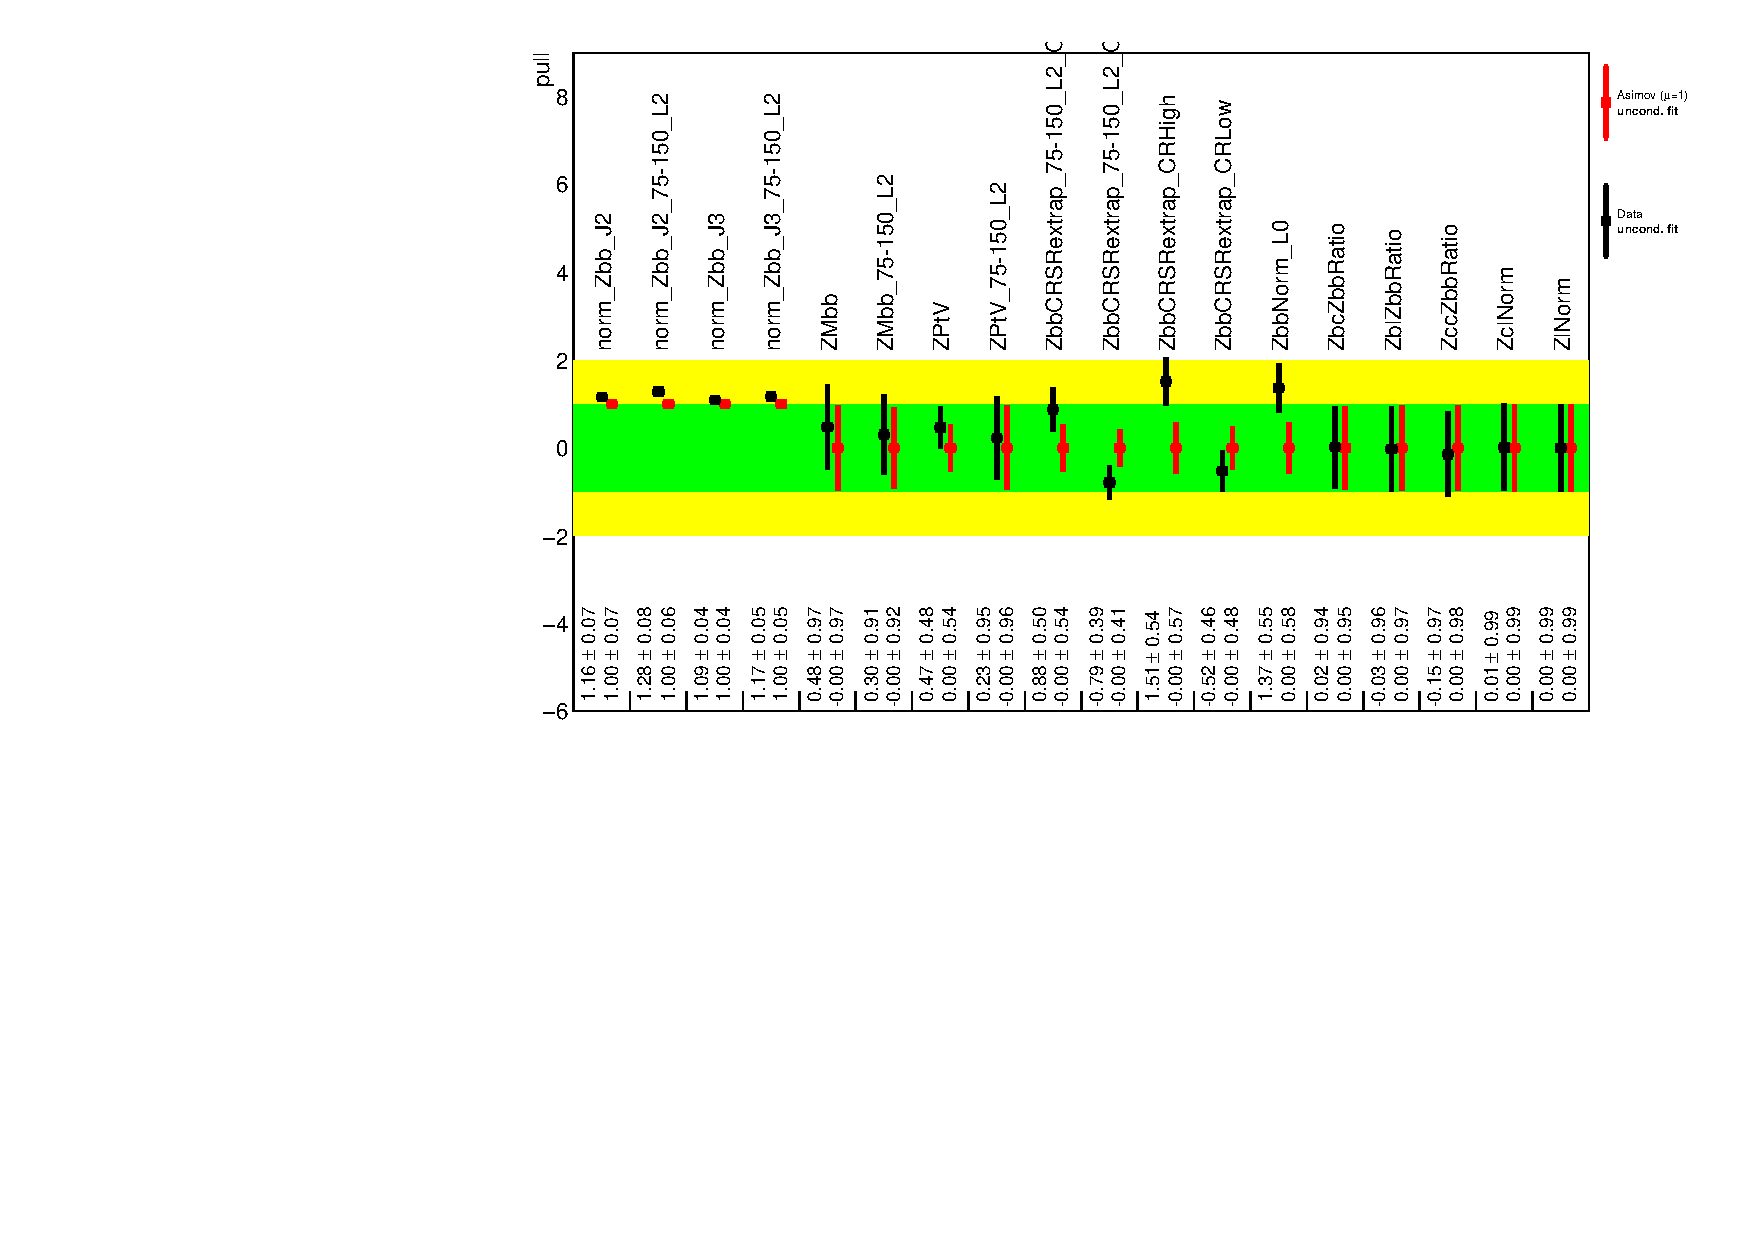
\includegraphics[width=0.49\linewidth]{final_fit_mva/pullComparisons/NP_Zjets.pdf}
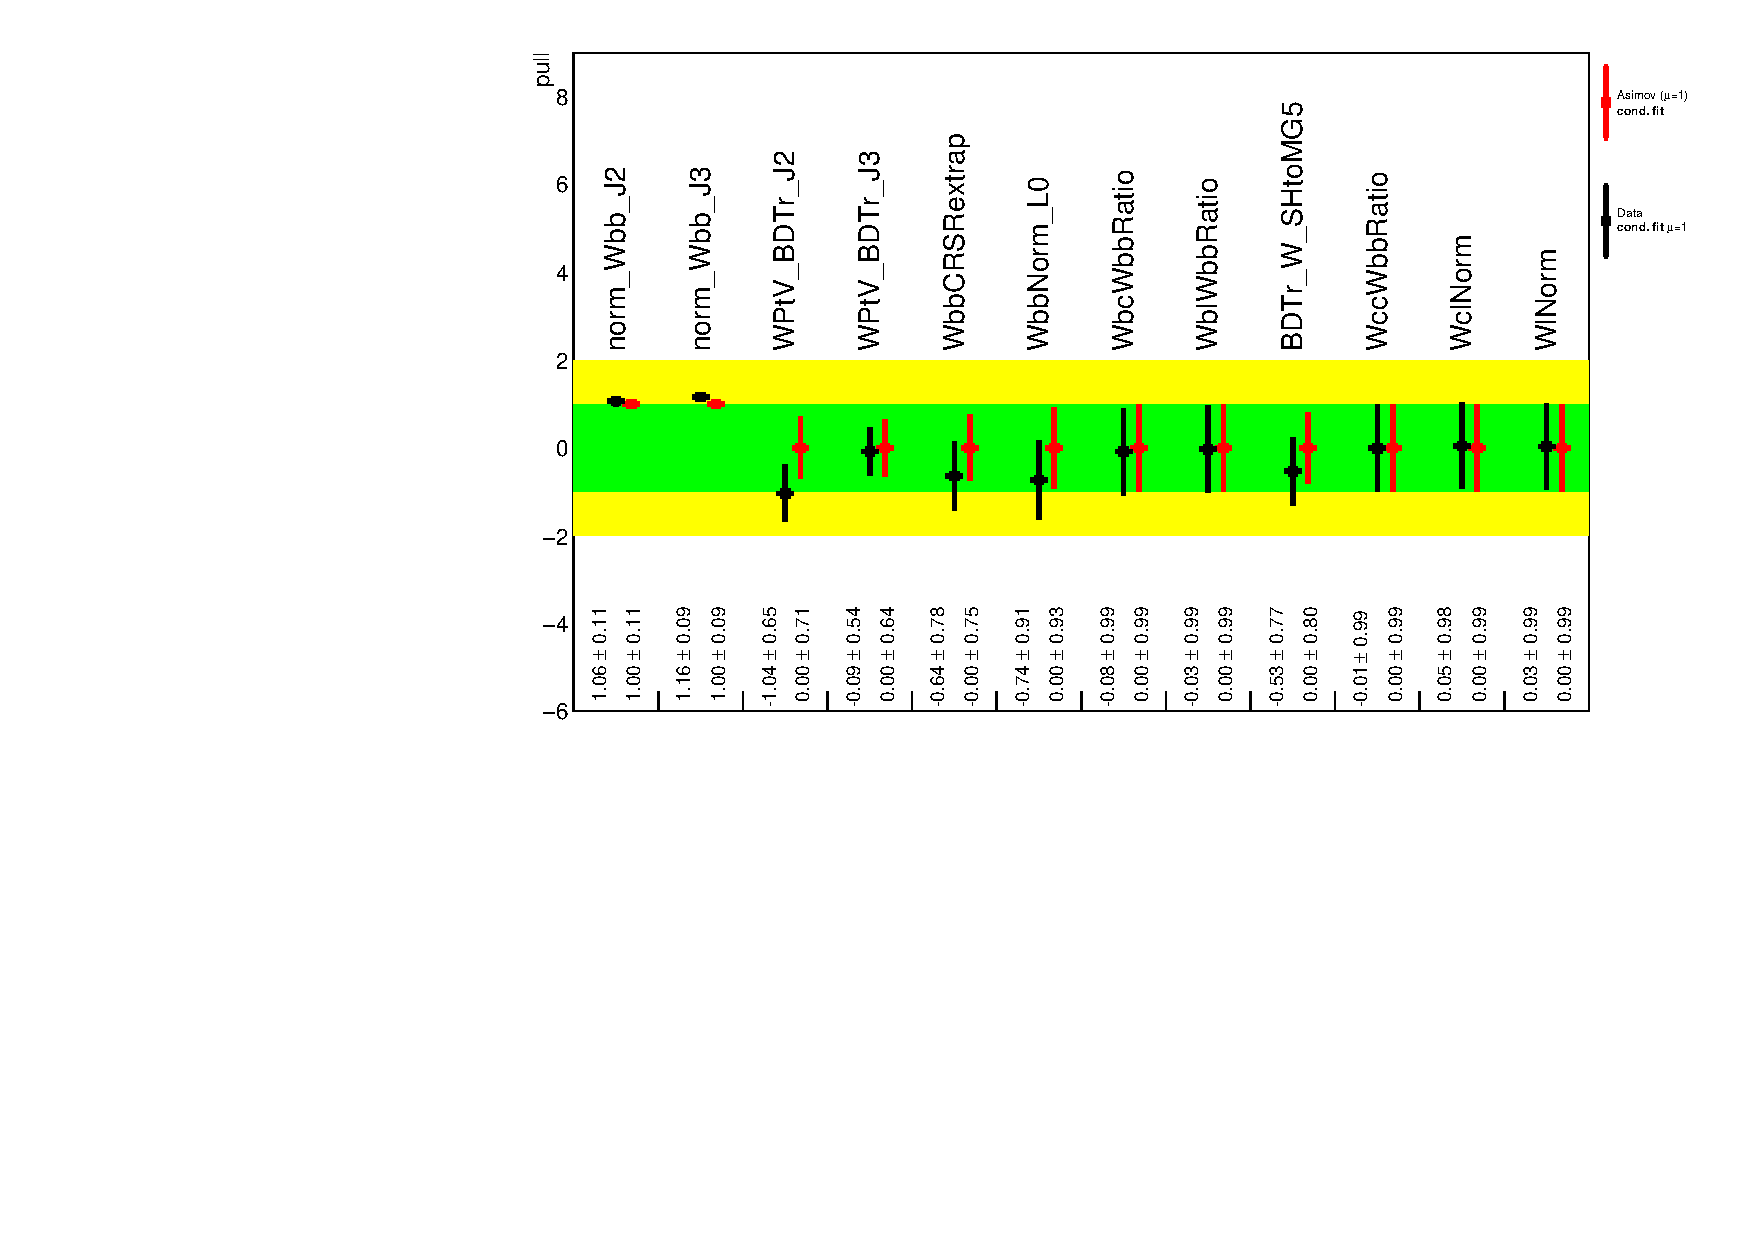
\includegraphics[width=0.49\linewidth]{final_fit_mva/pullComparisons/NP_Wjets.pdf}
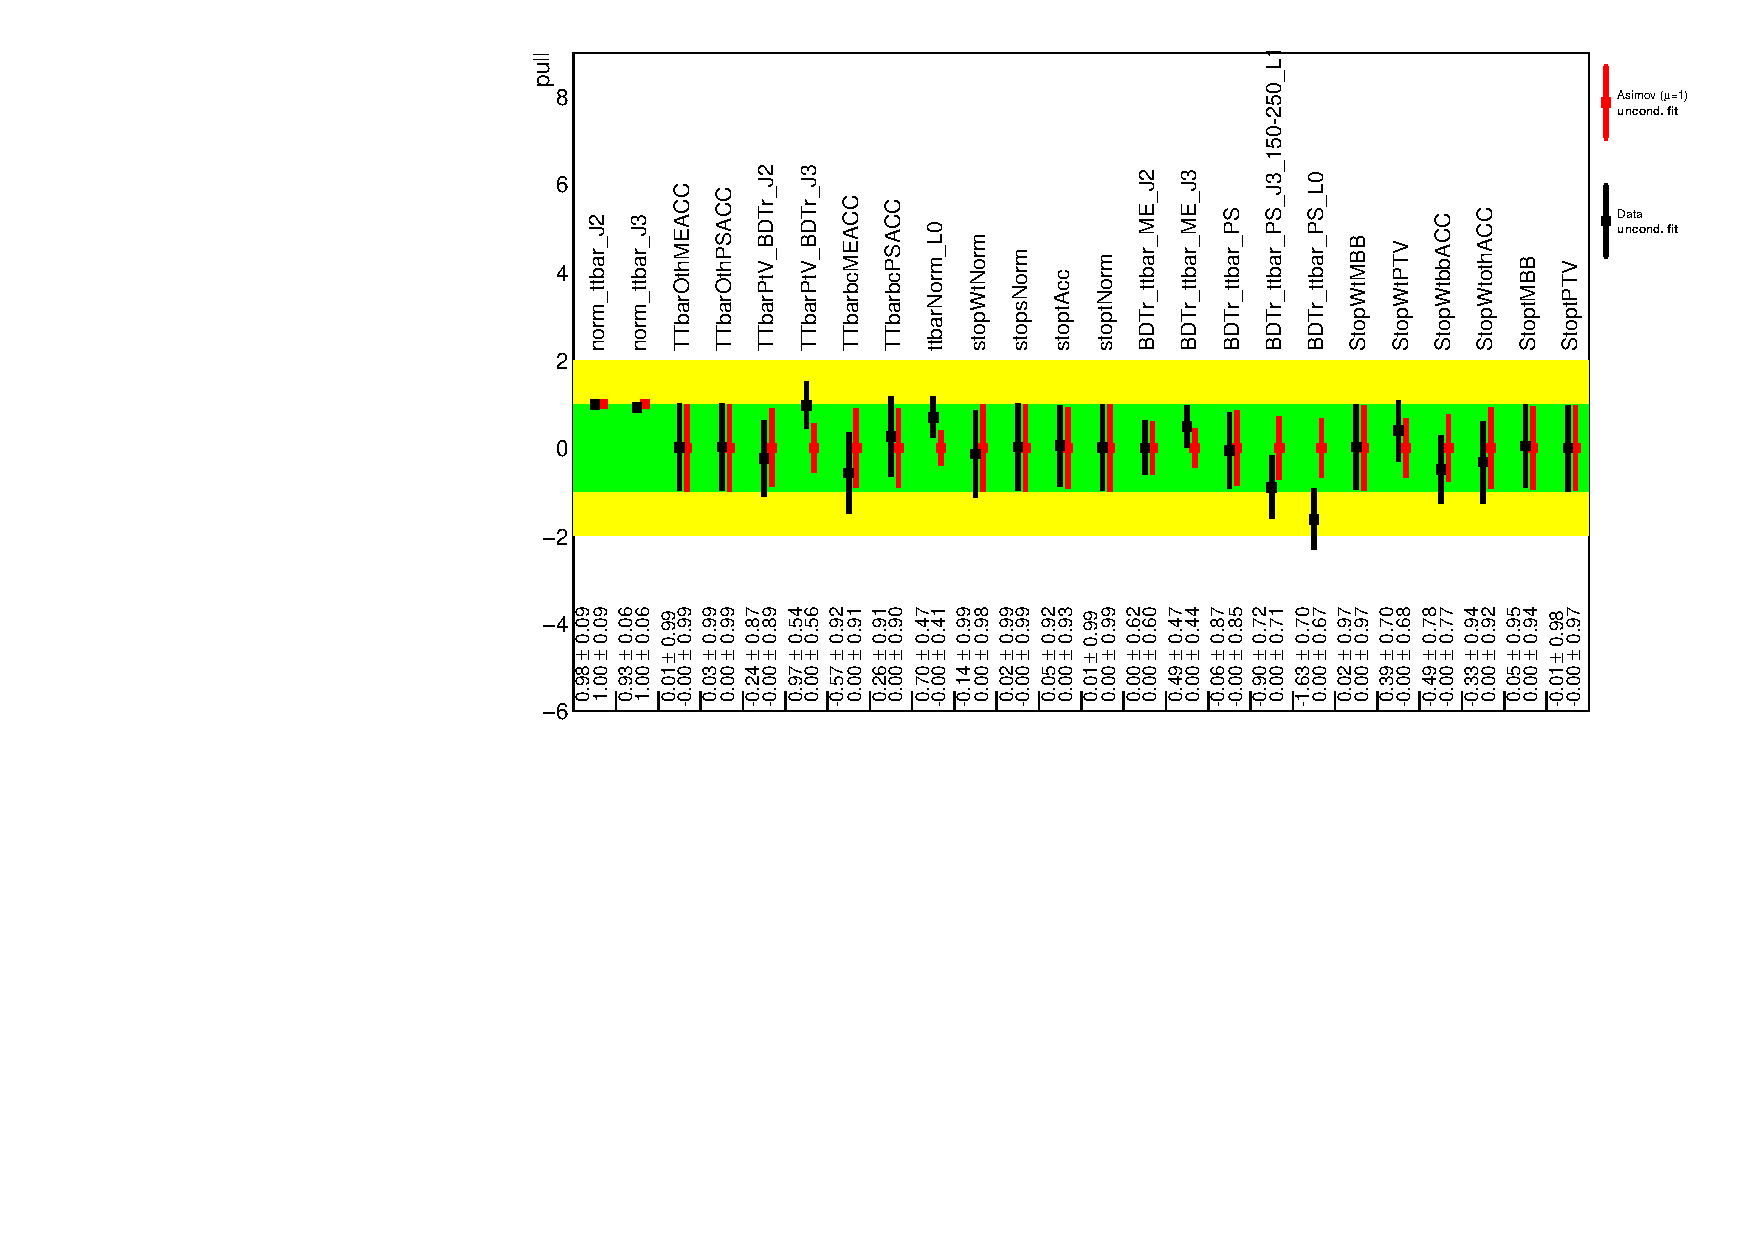
\includegraphics[width=0.49\linewidth]{final_fit_mva/pullComparisons/NP_Top.pdf}
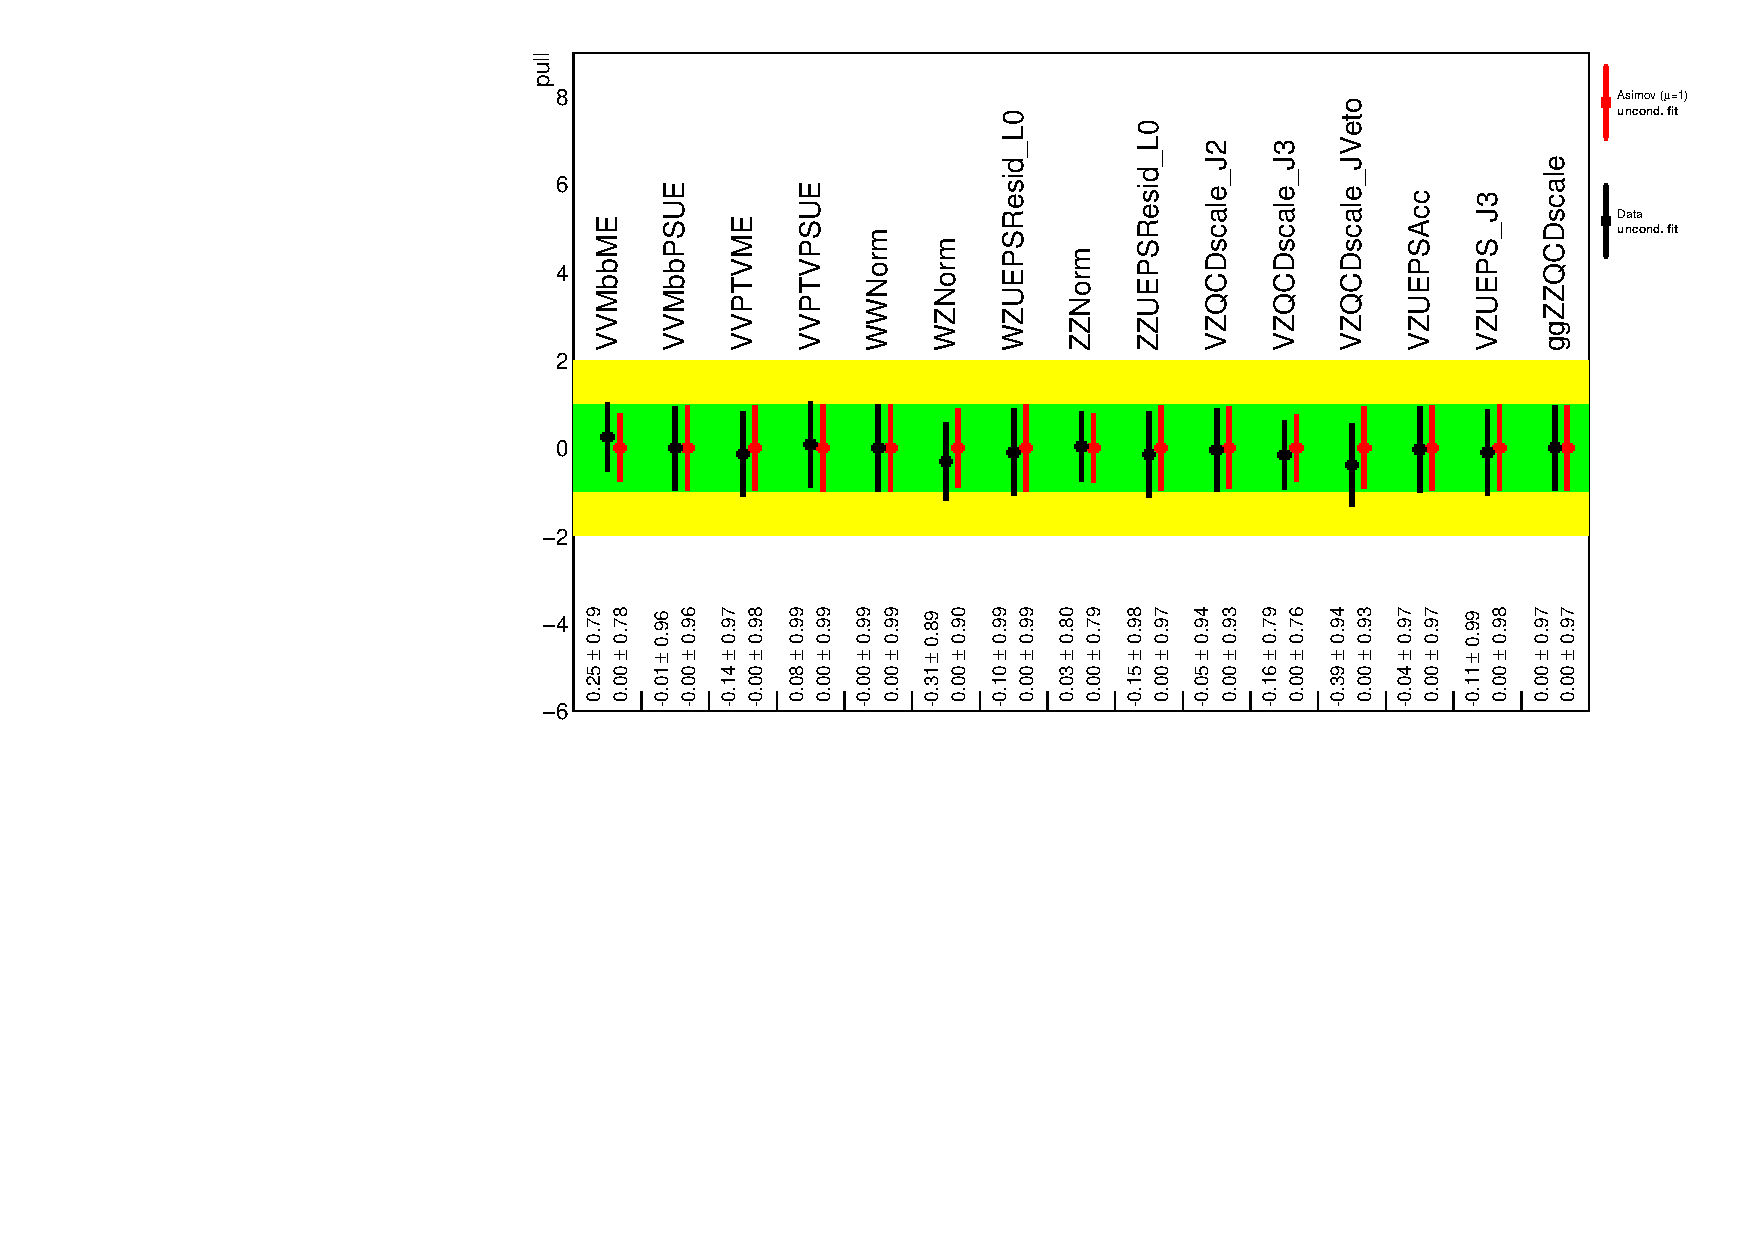
\includegraphics[width=0.49\linewidth]{final_fit_mva/pullComparisons/NP_Diboson.pdf}
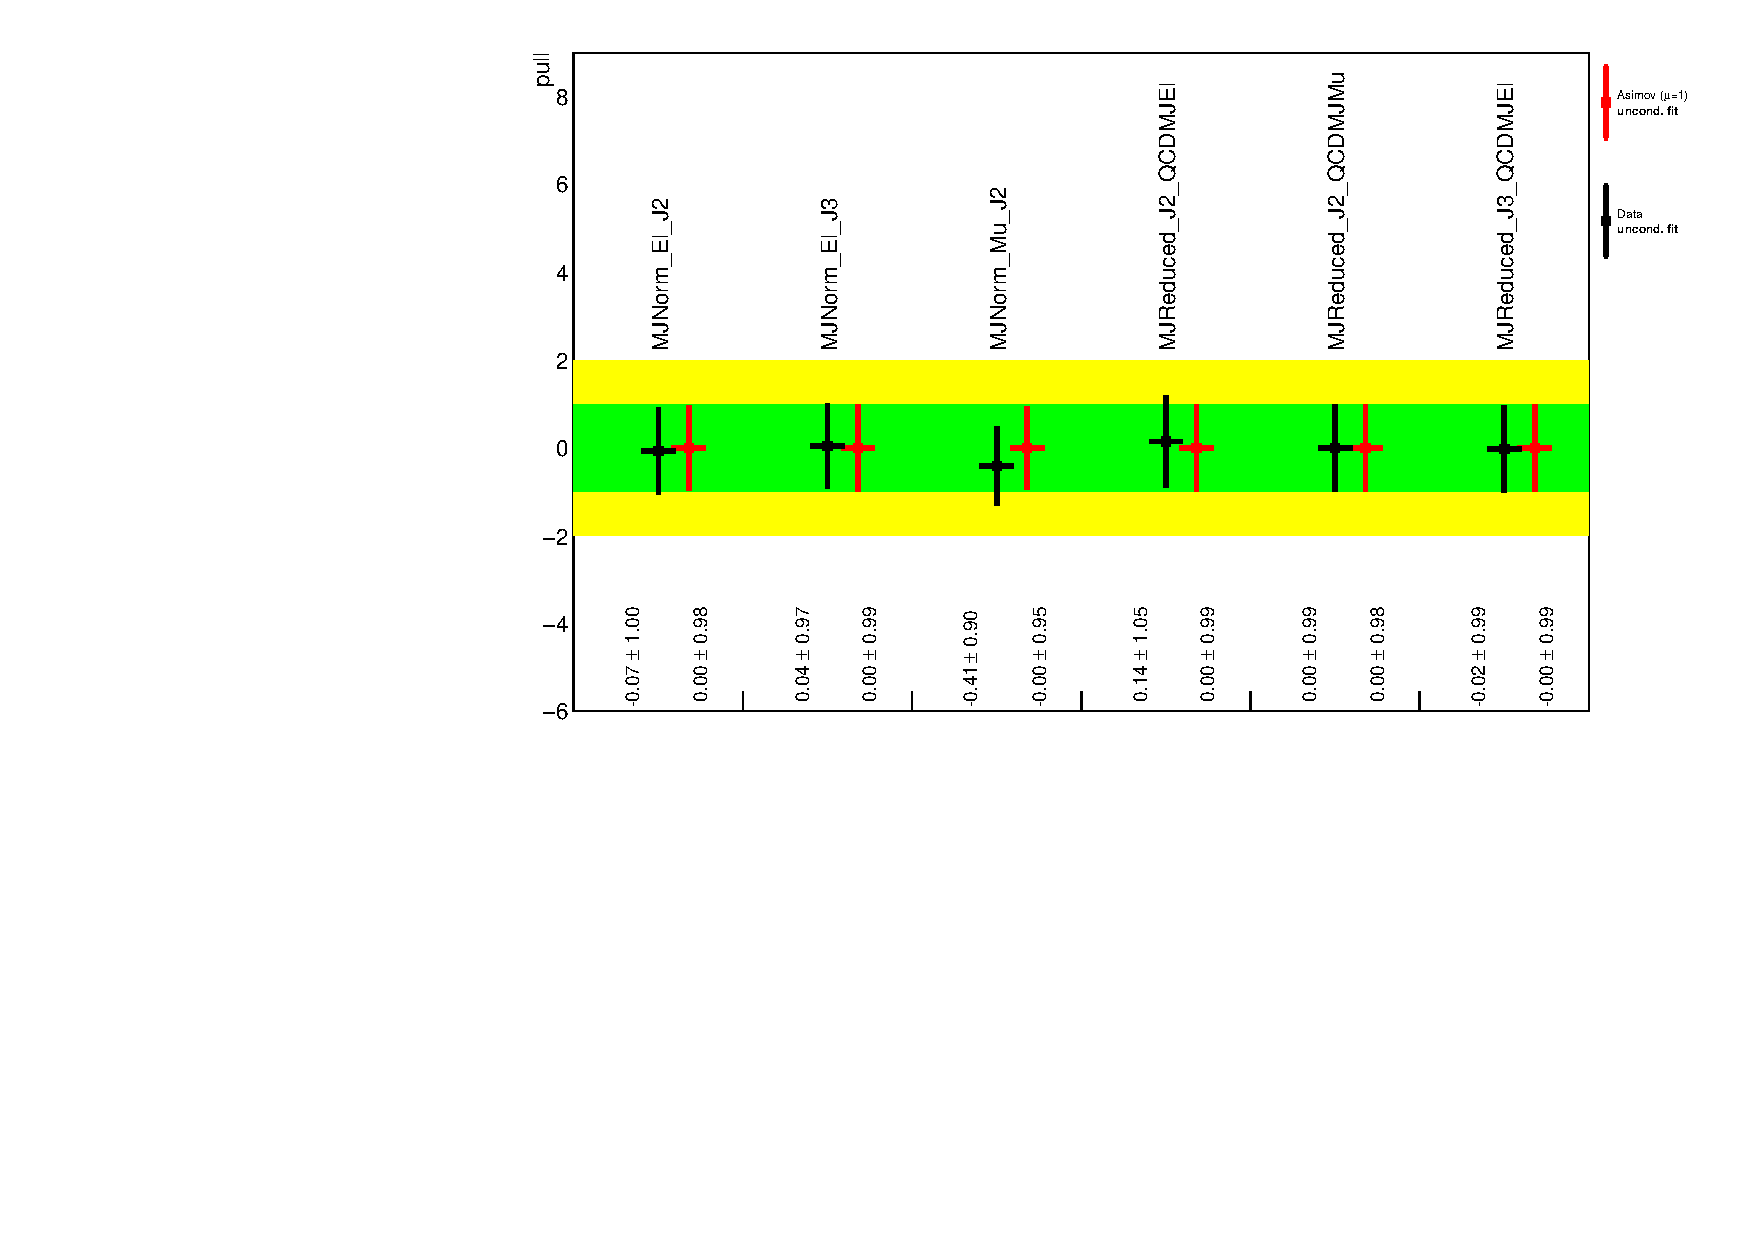
\includegraphics[width=0.49\linewidth]{final_fit_mva/pullComparisons/NP_MJ.pdf}
\caption{caption}
% MC modelling, multi-jet estimate nuisance parameter pulls and the free parameter
% scale factors corresponding to a conditional combined fit performed to Asimov
% dataset (red) and an unconditional combined fit to the \RunTwo data (black).
\label{fig:nppulls_012L_MVAVH_a} 
\end{figure}
%
\begin{figure}[hb]
\centering
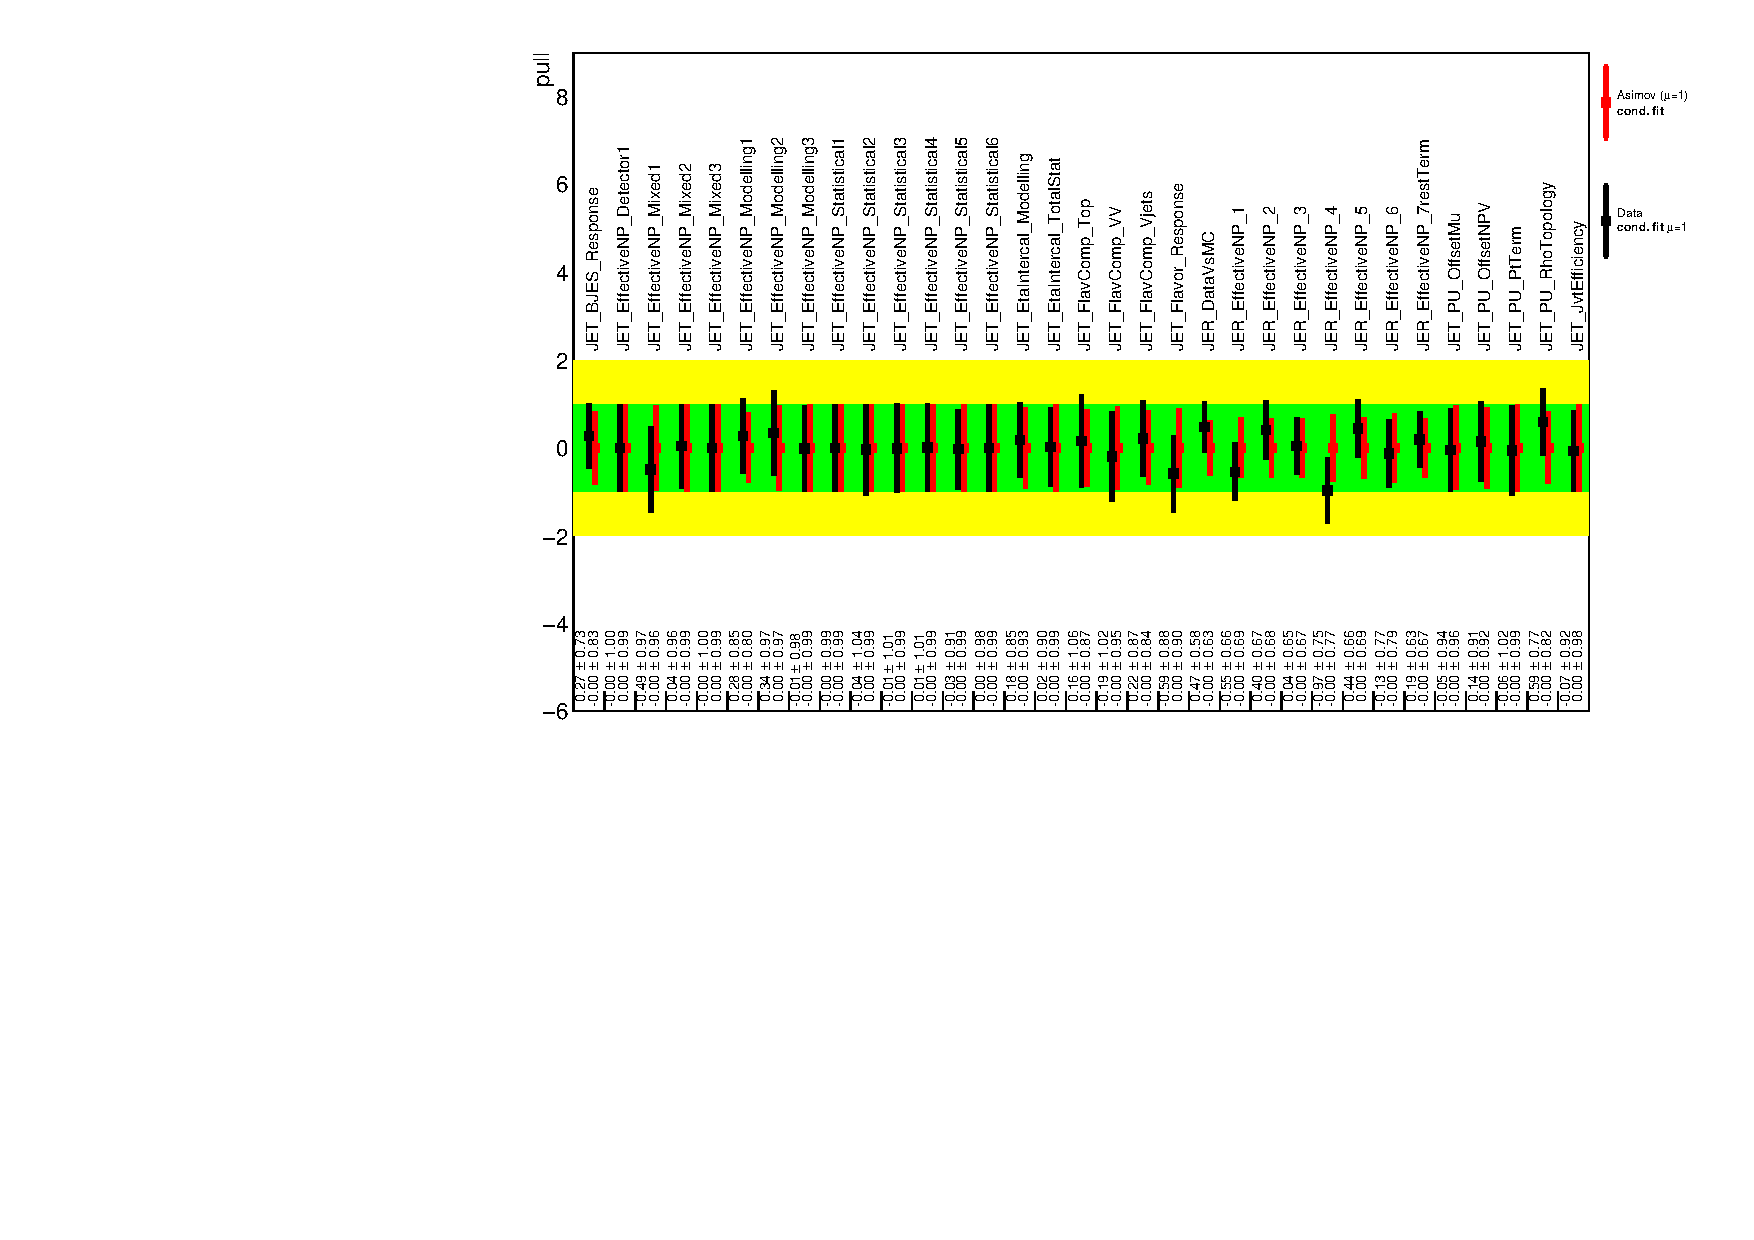
\includegraphics[width=0.49\linewidth]{final_fit_mva/pullComparisons/NP_Jet.pdf}
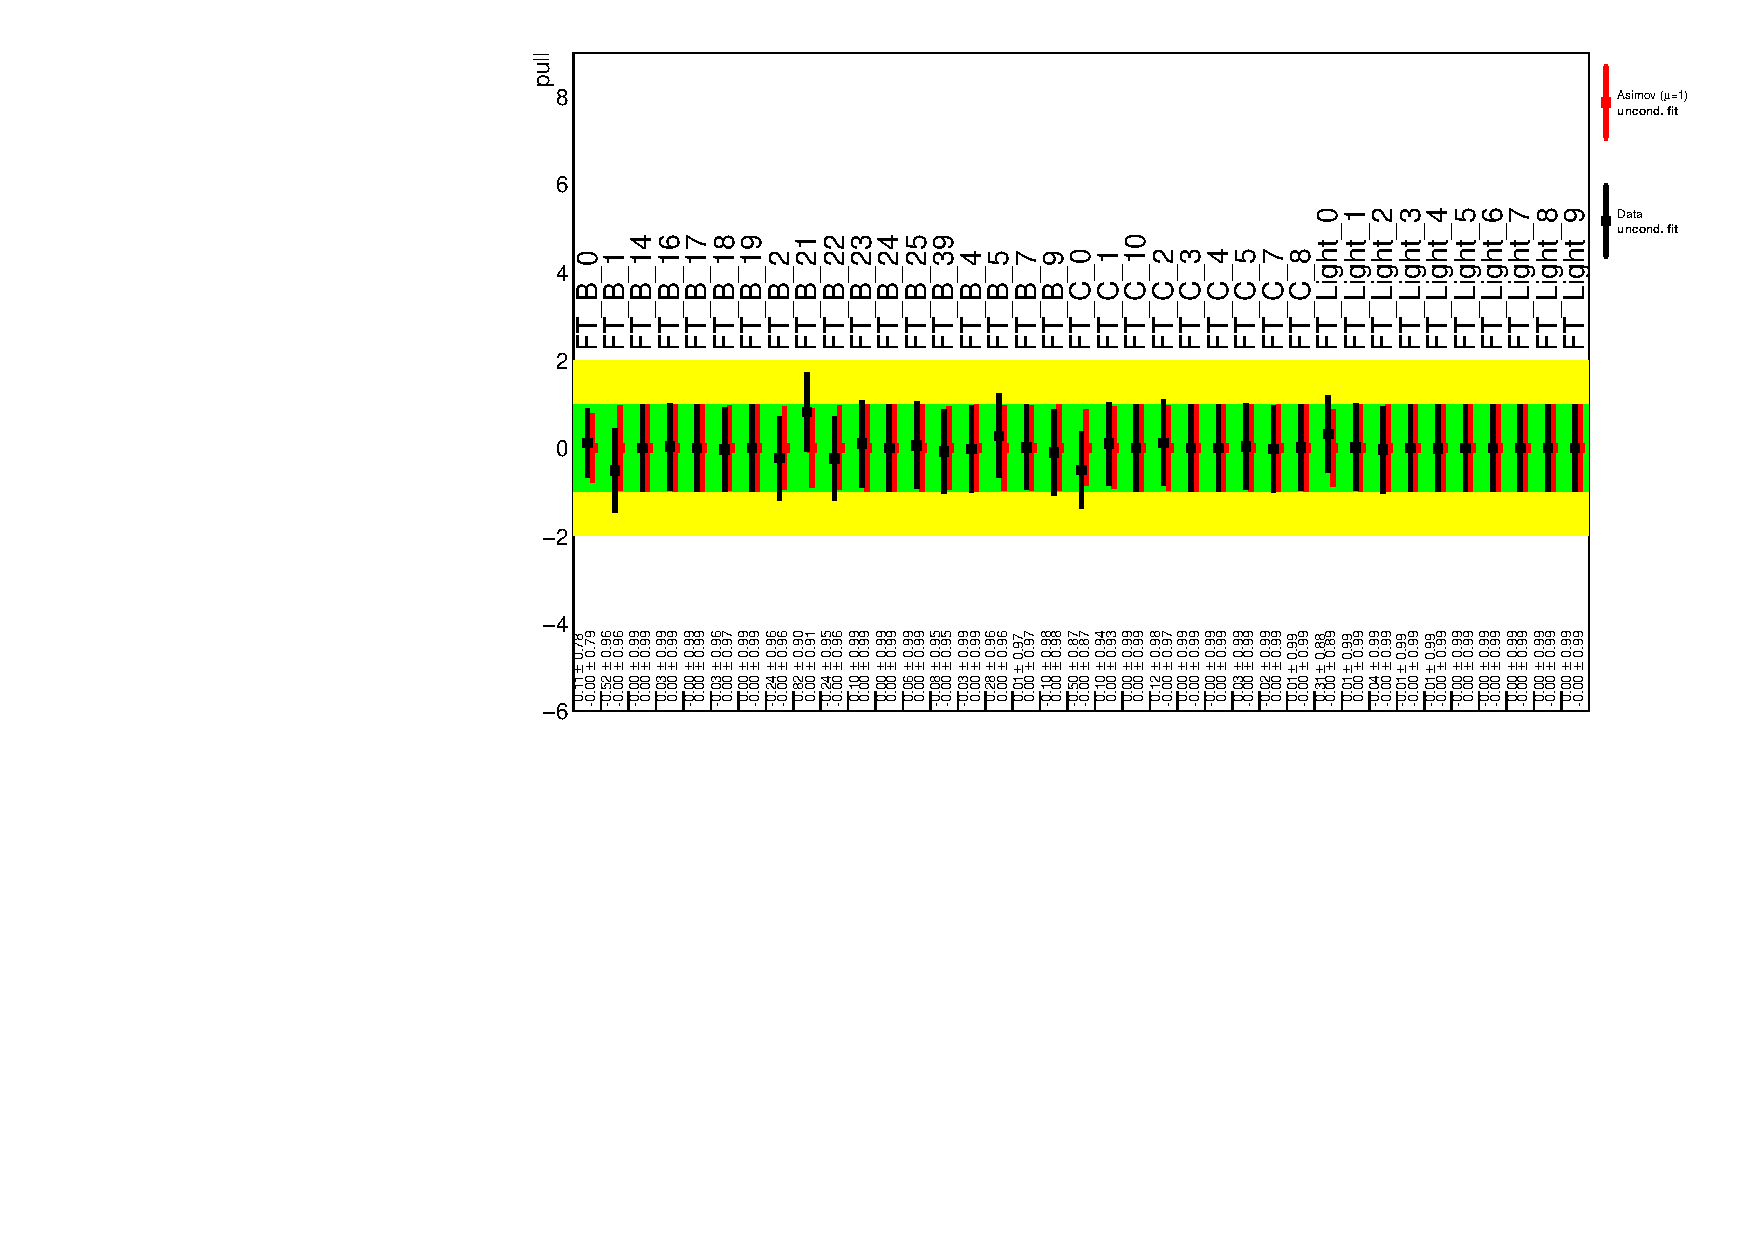
\includegraphics[width=0.49\linewidth]{final_fit_mva/pullComparisons/NP_BTag.pdf}
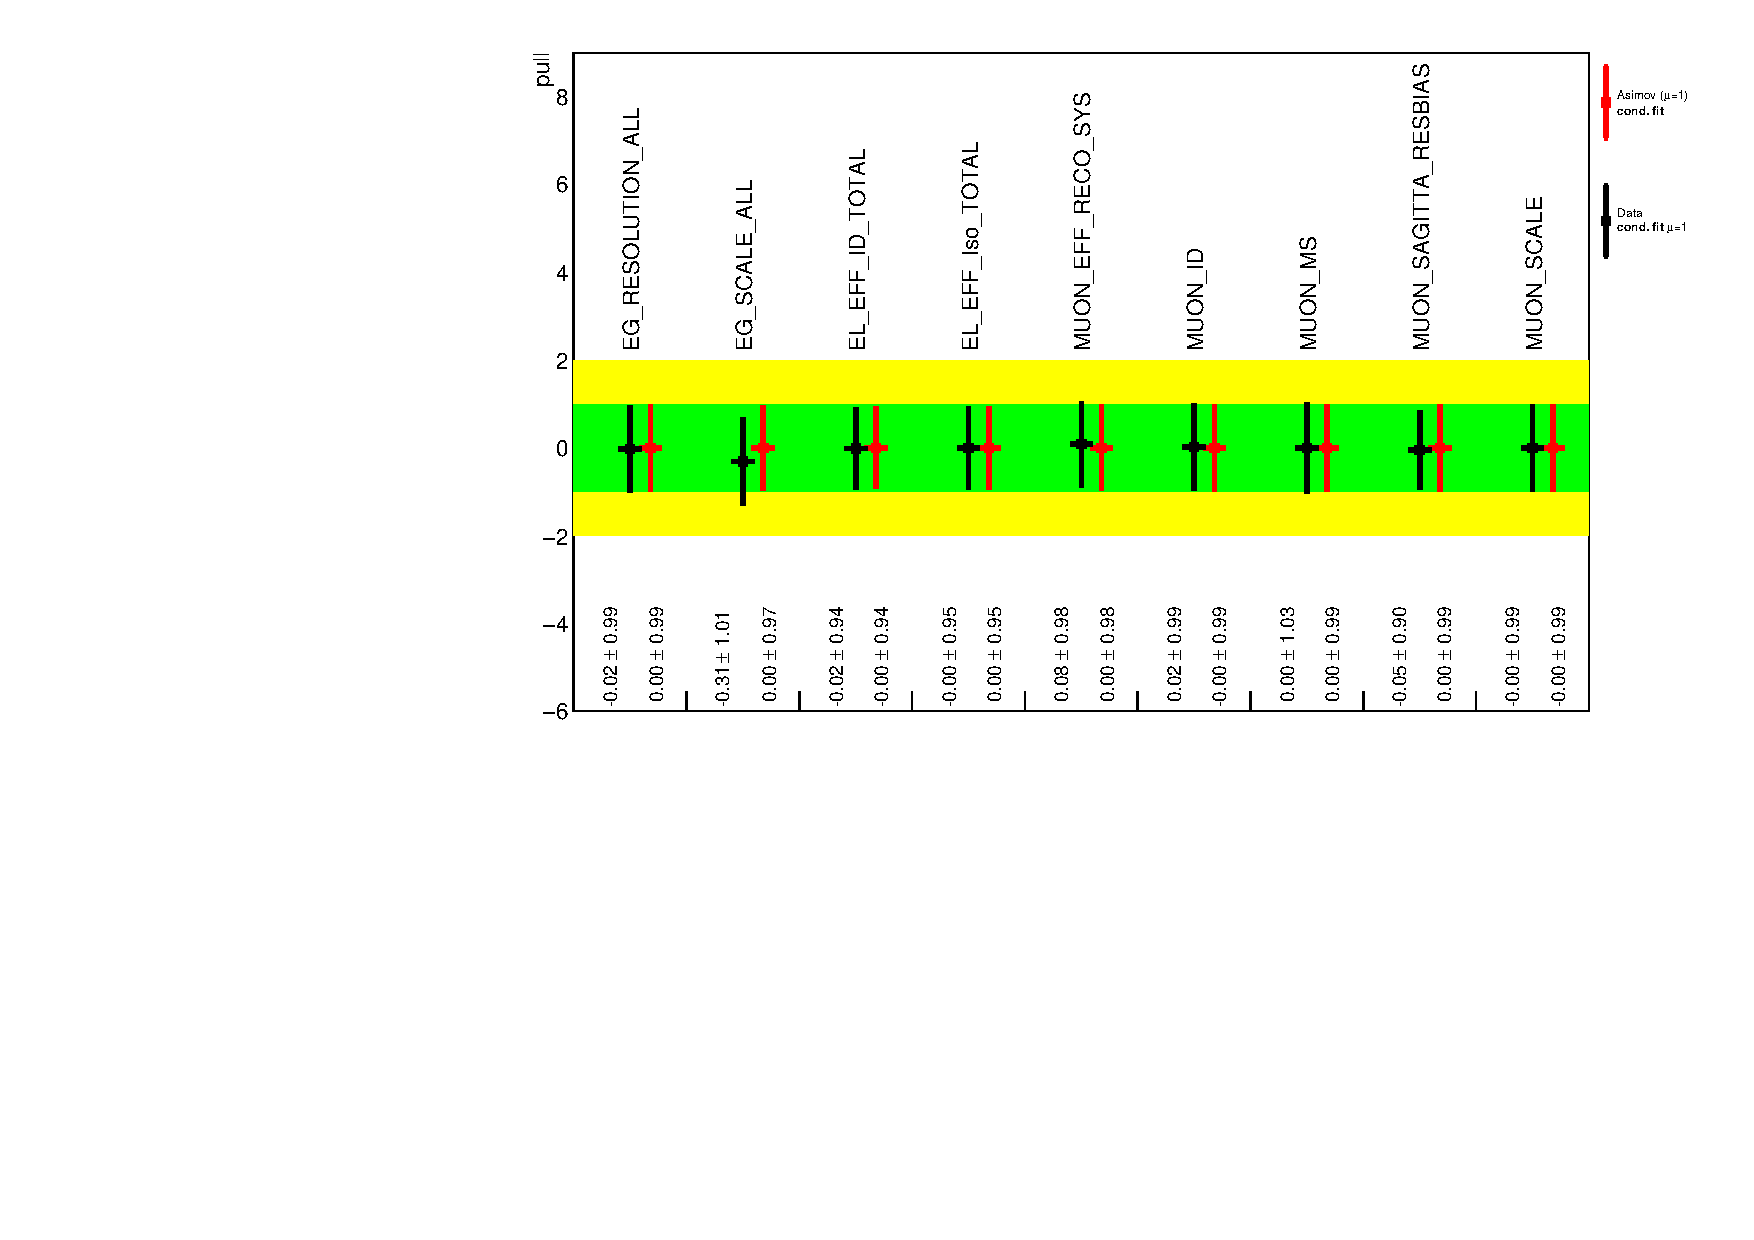
\includegraphics[width=0.49\linewidth]{final_fit_mva/pullComparisons/NP_Lepton.pdf}
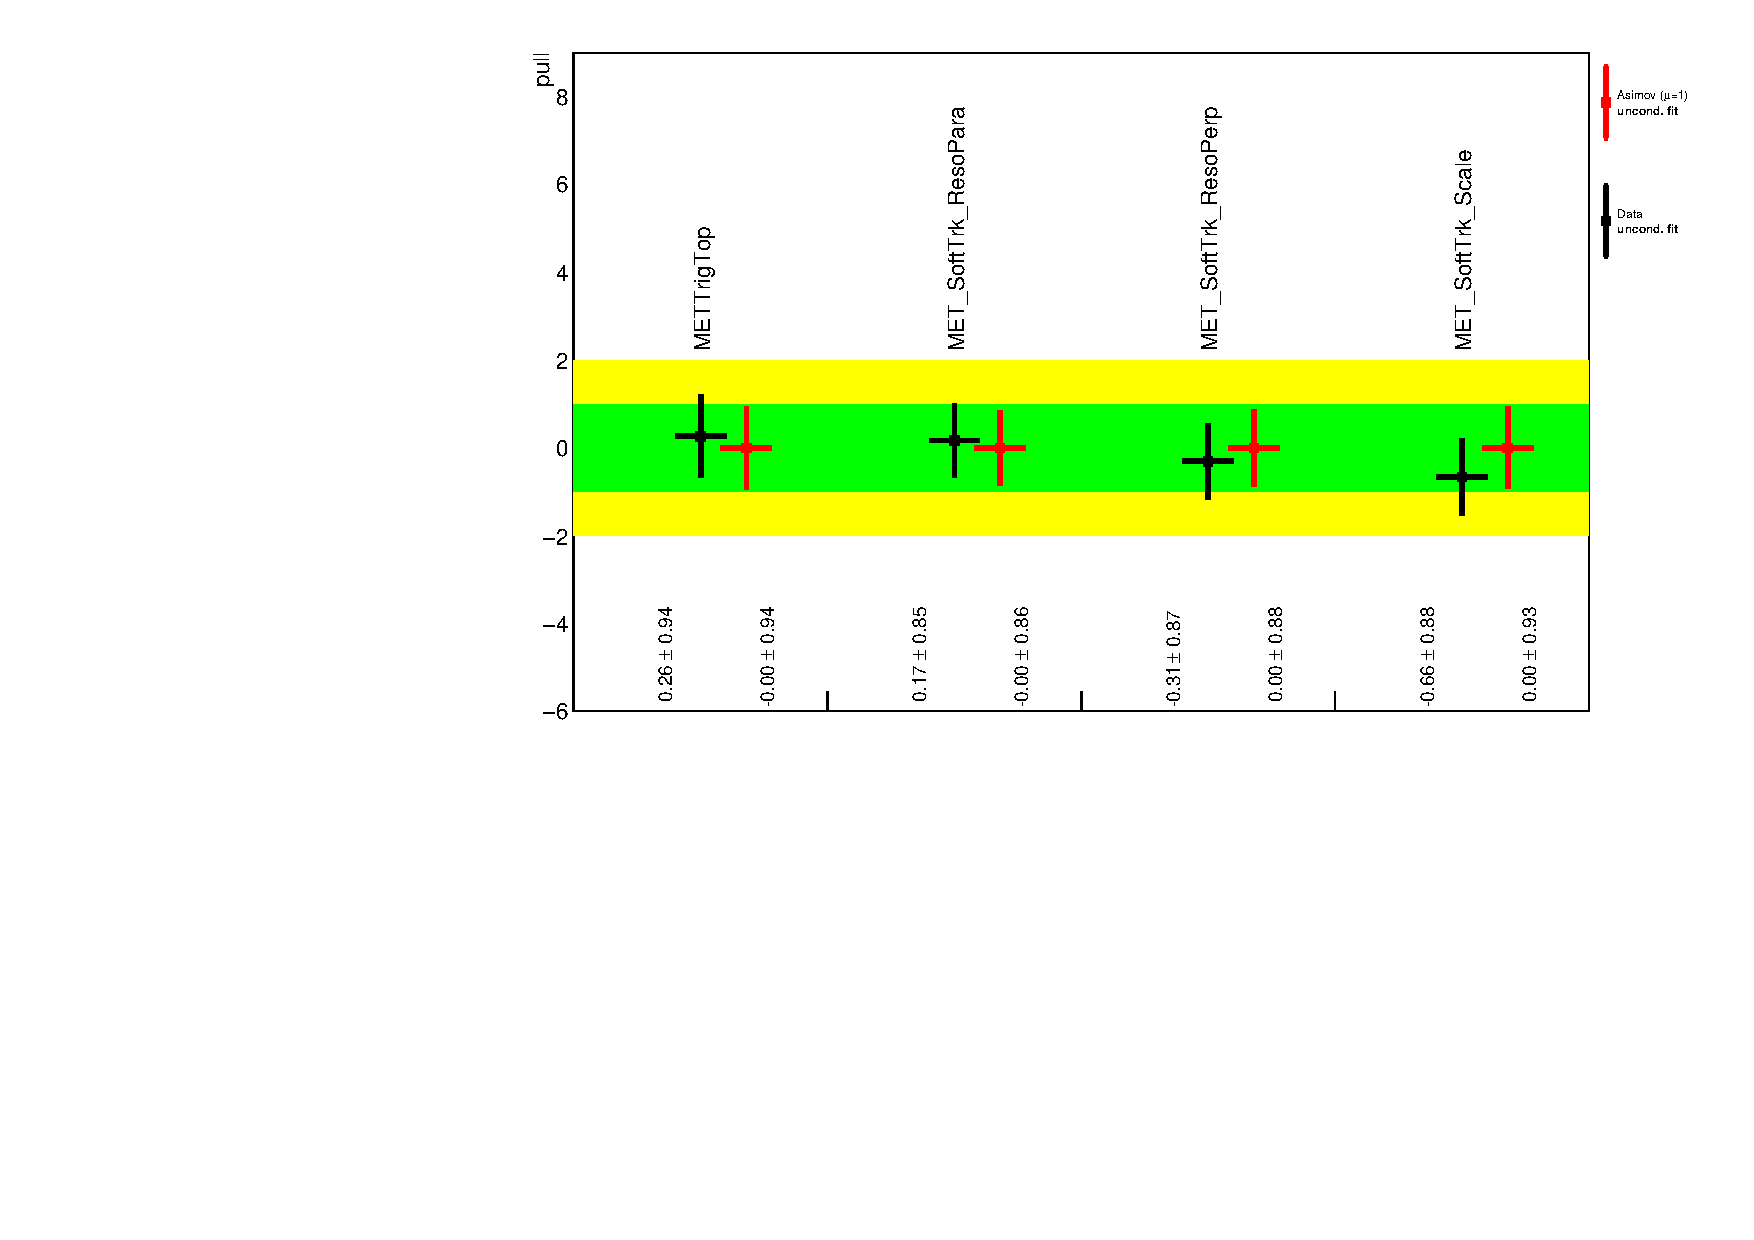
\includegraphics[width=0.49\linewidth]{final_fit_mva/pullComparisons/NP_MET.pdf}
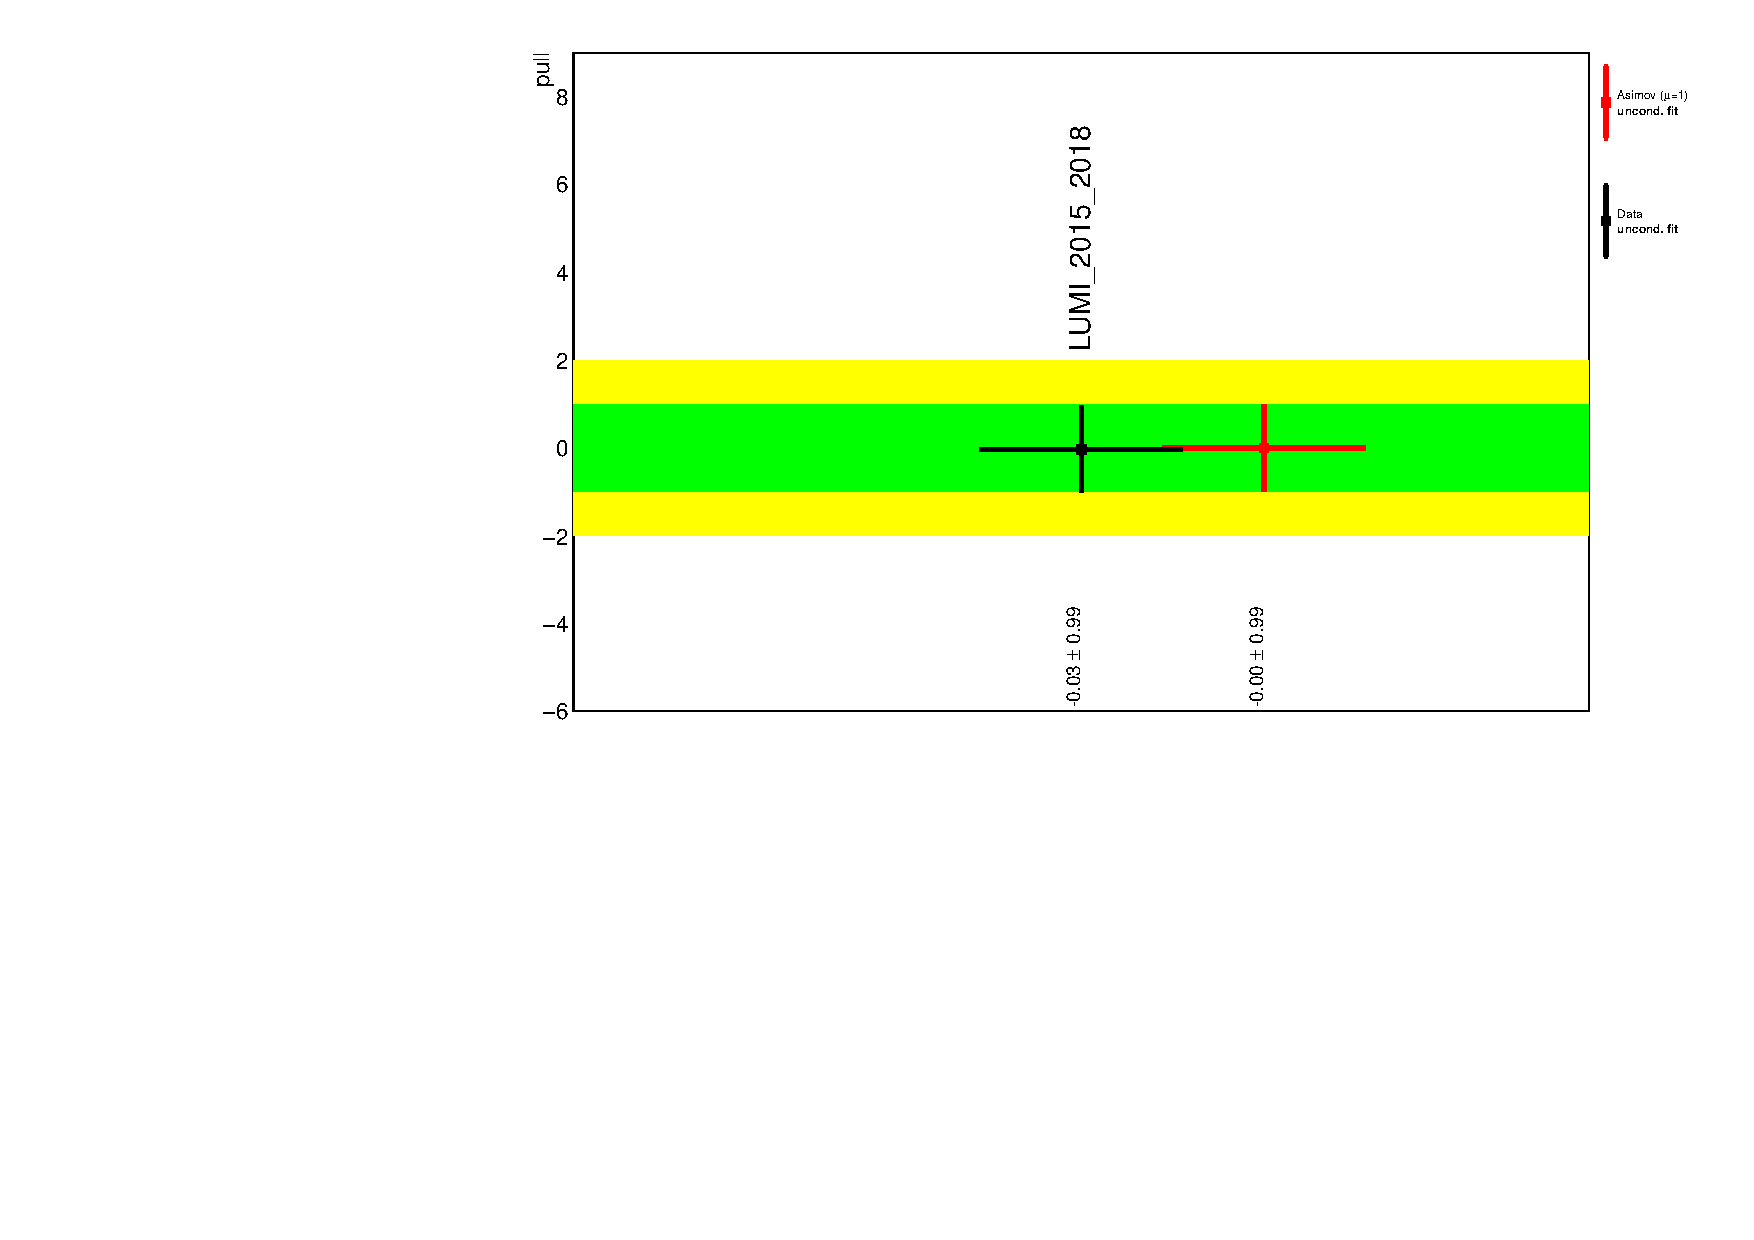
\includegraphics[width=0.49\linewidth]{final_fit_mva/pullComparisons/NP_LUMI.pdf}
\caption{caption}
% Detector and luminosity nuisance parameter pulls corresponding to a conditional
% combined fit performed to an Asimov dataset (red) and an unconditional combined
% fit to the \RunTwo data (black)
\label{fig:nppulls_012L_MVAVH_b}
\end{figure}
%
% \begin{figure}[hb]
% \centering
% 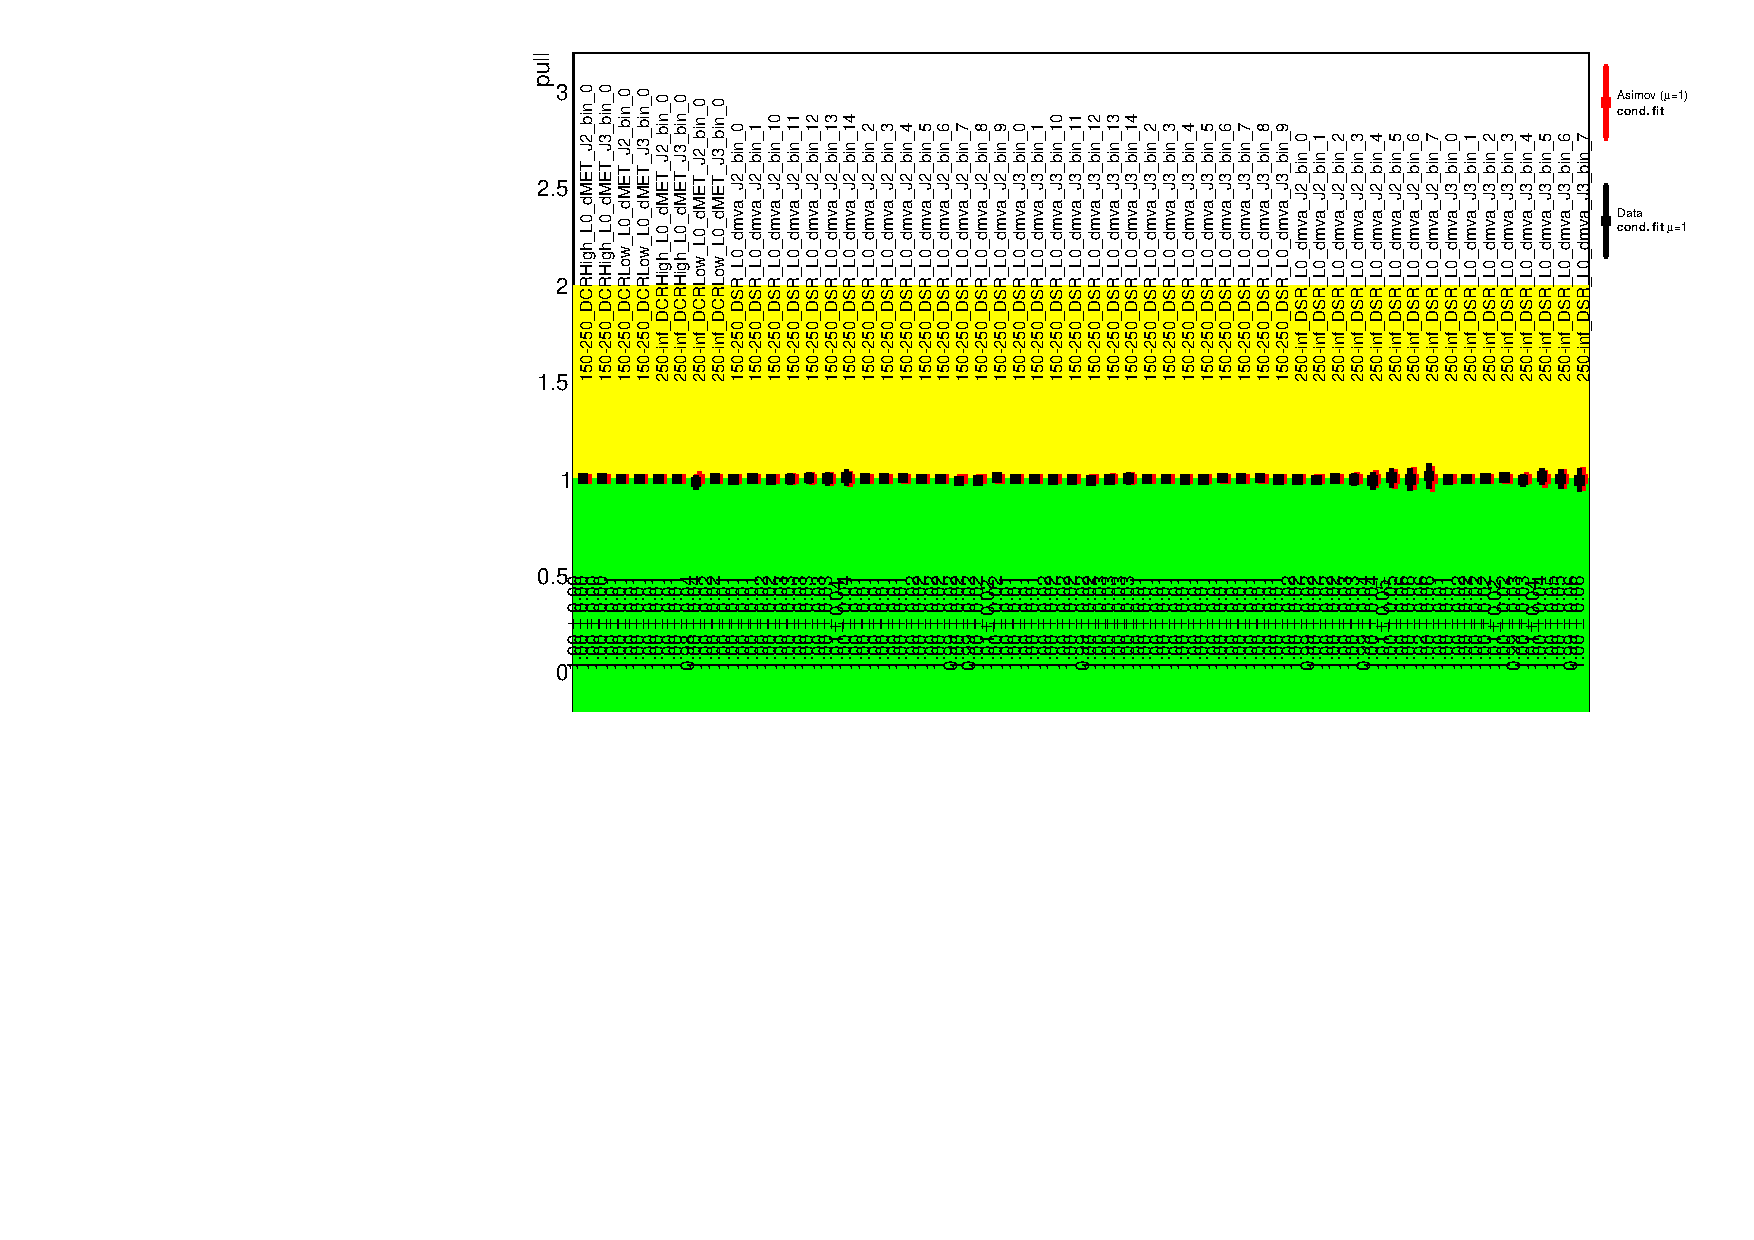
\includegraphics[width=0.49\linewidth]{final_fit_mva/pullComparisons/NP_GammasL0.pdf}
% 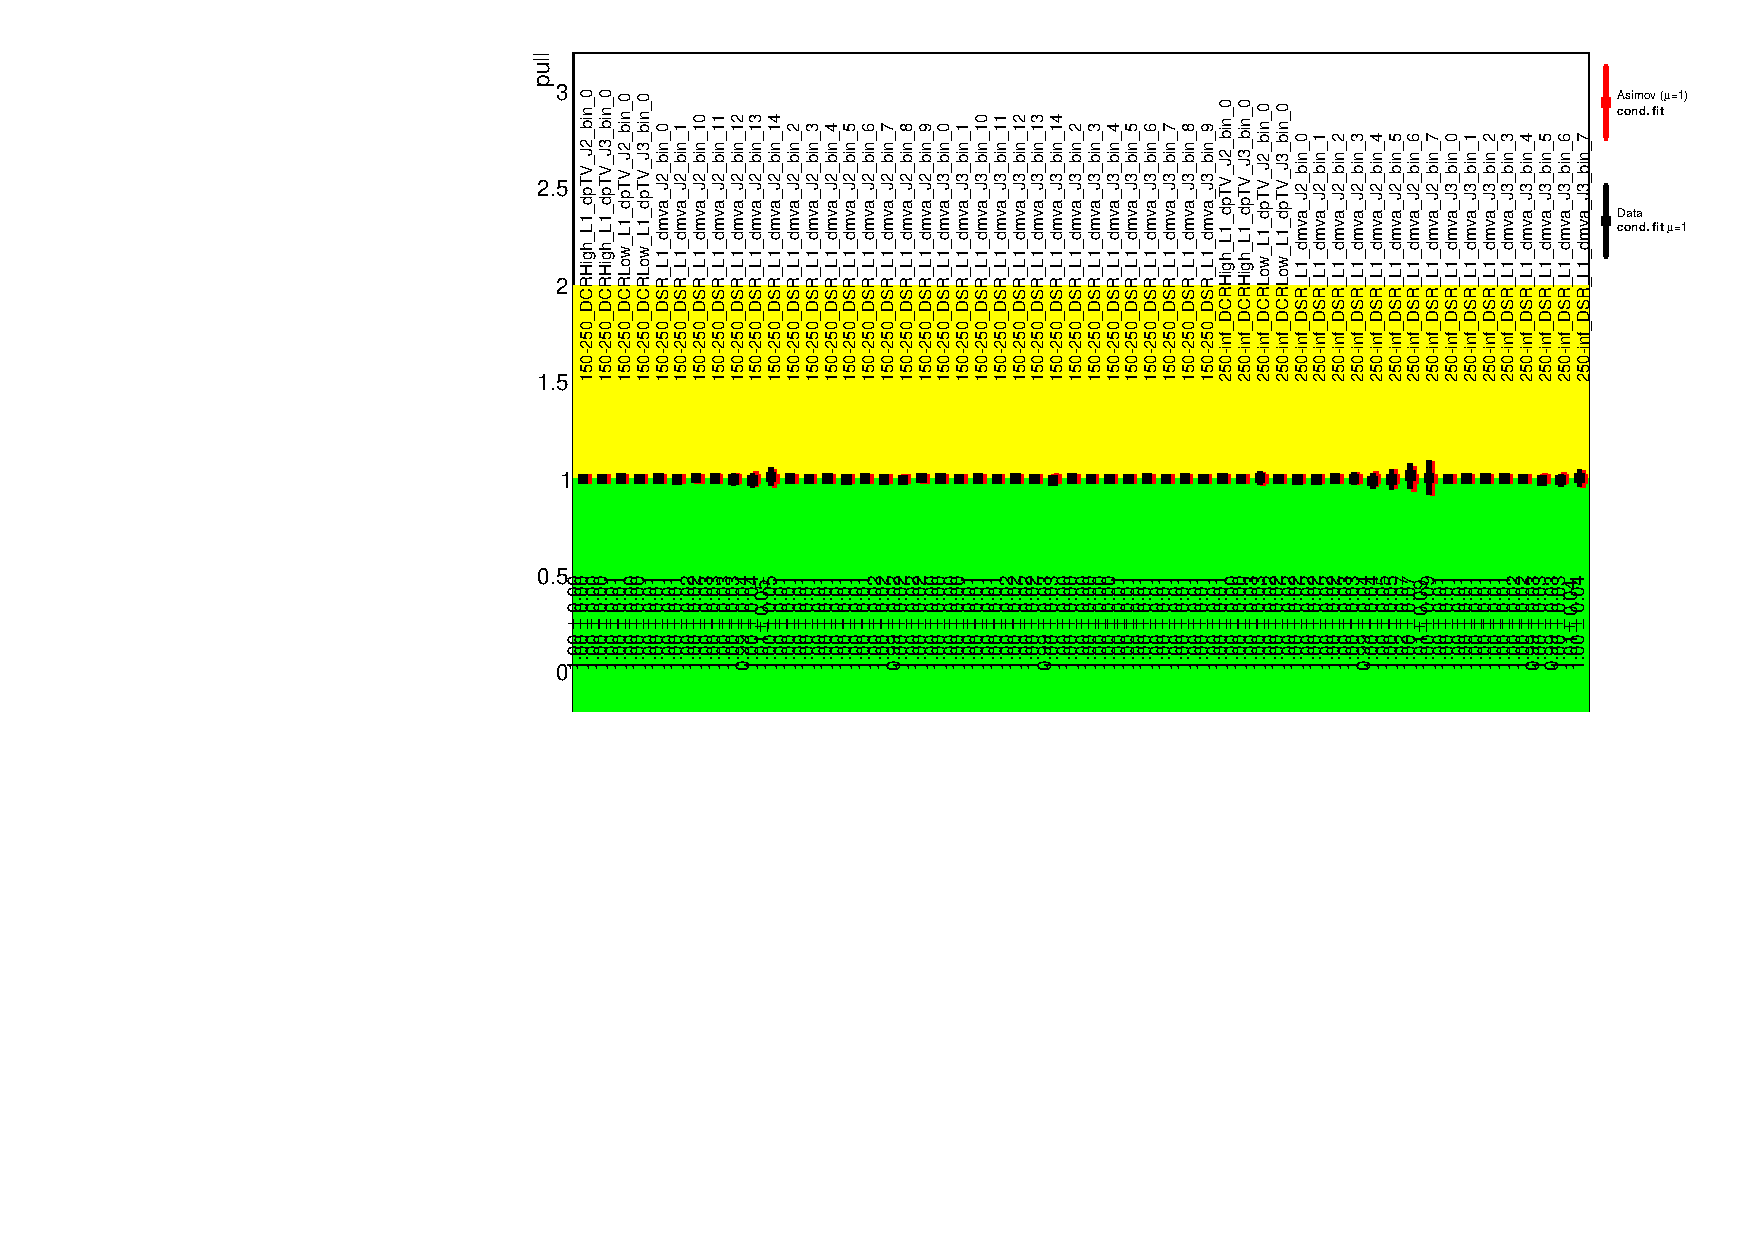
\includegraphics[width=0.49\linewidth]{final_fit_mva/pullComparisons/NP_GammasL1.pdf}
% 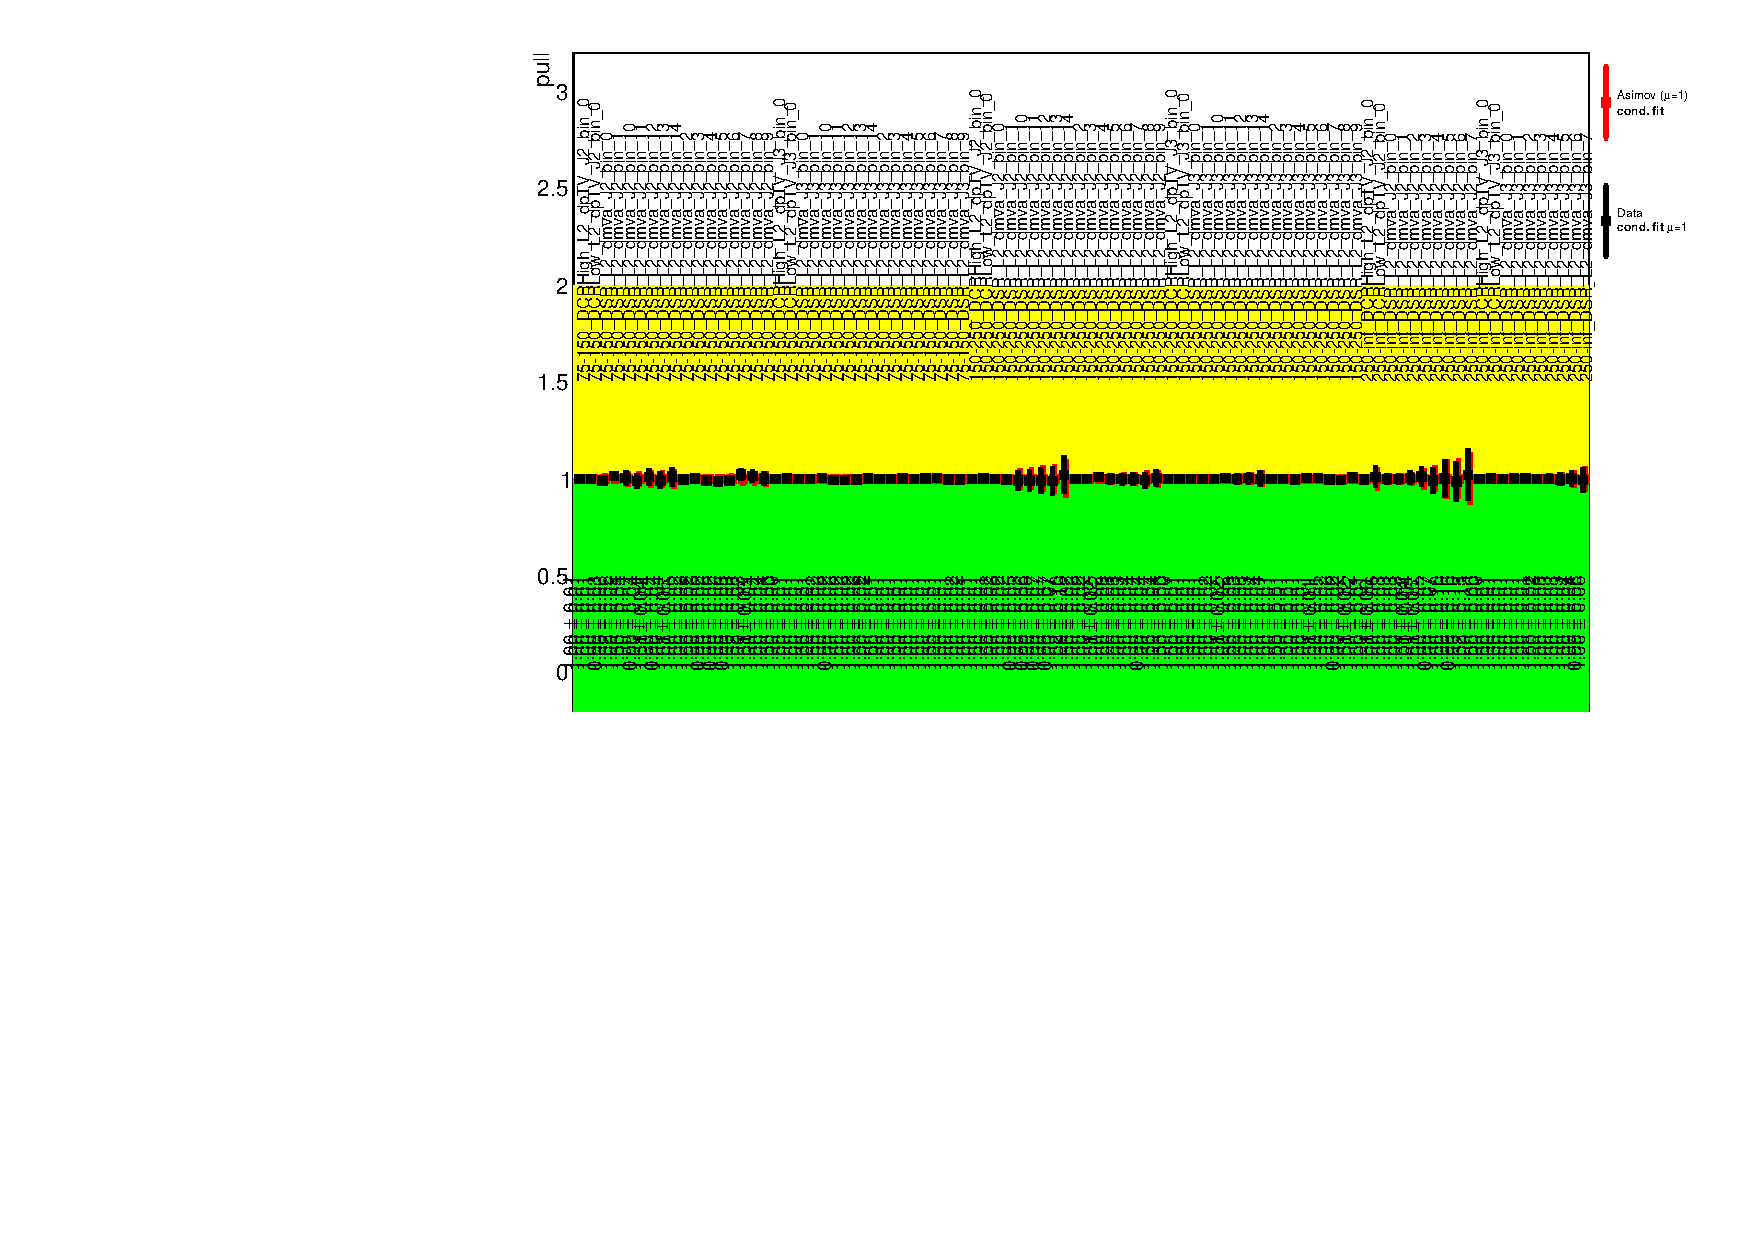
\includegraphics[width=0.49\linewidth]{final_fit_mva/pullComparisons/NP_GammasL2.pdf}
% 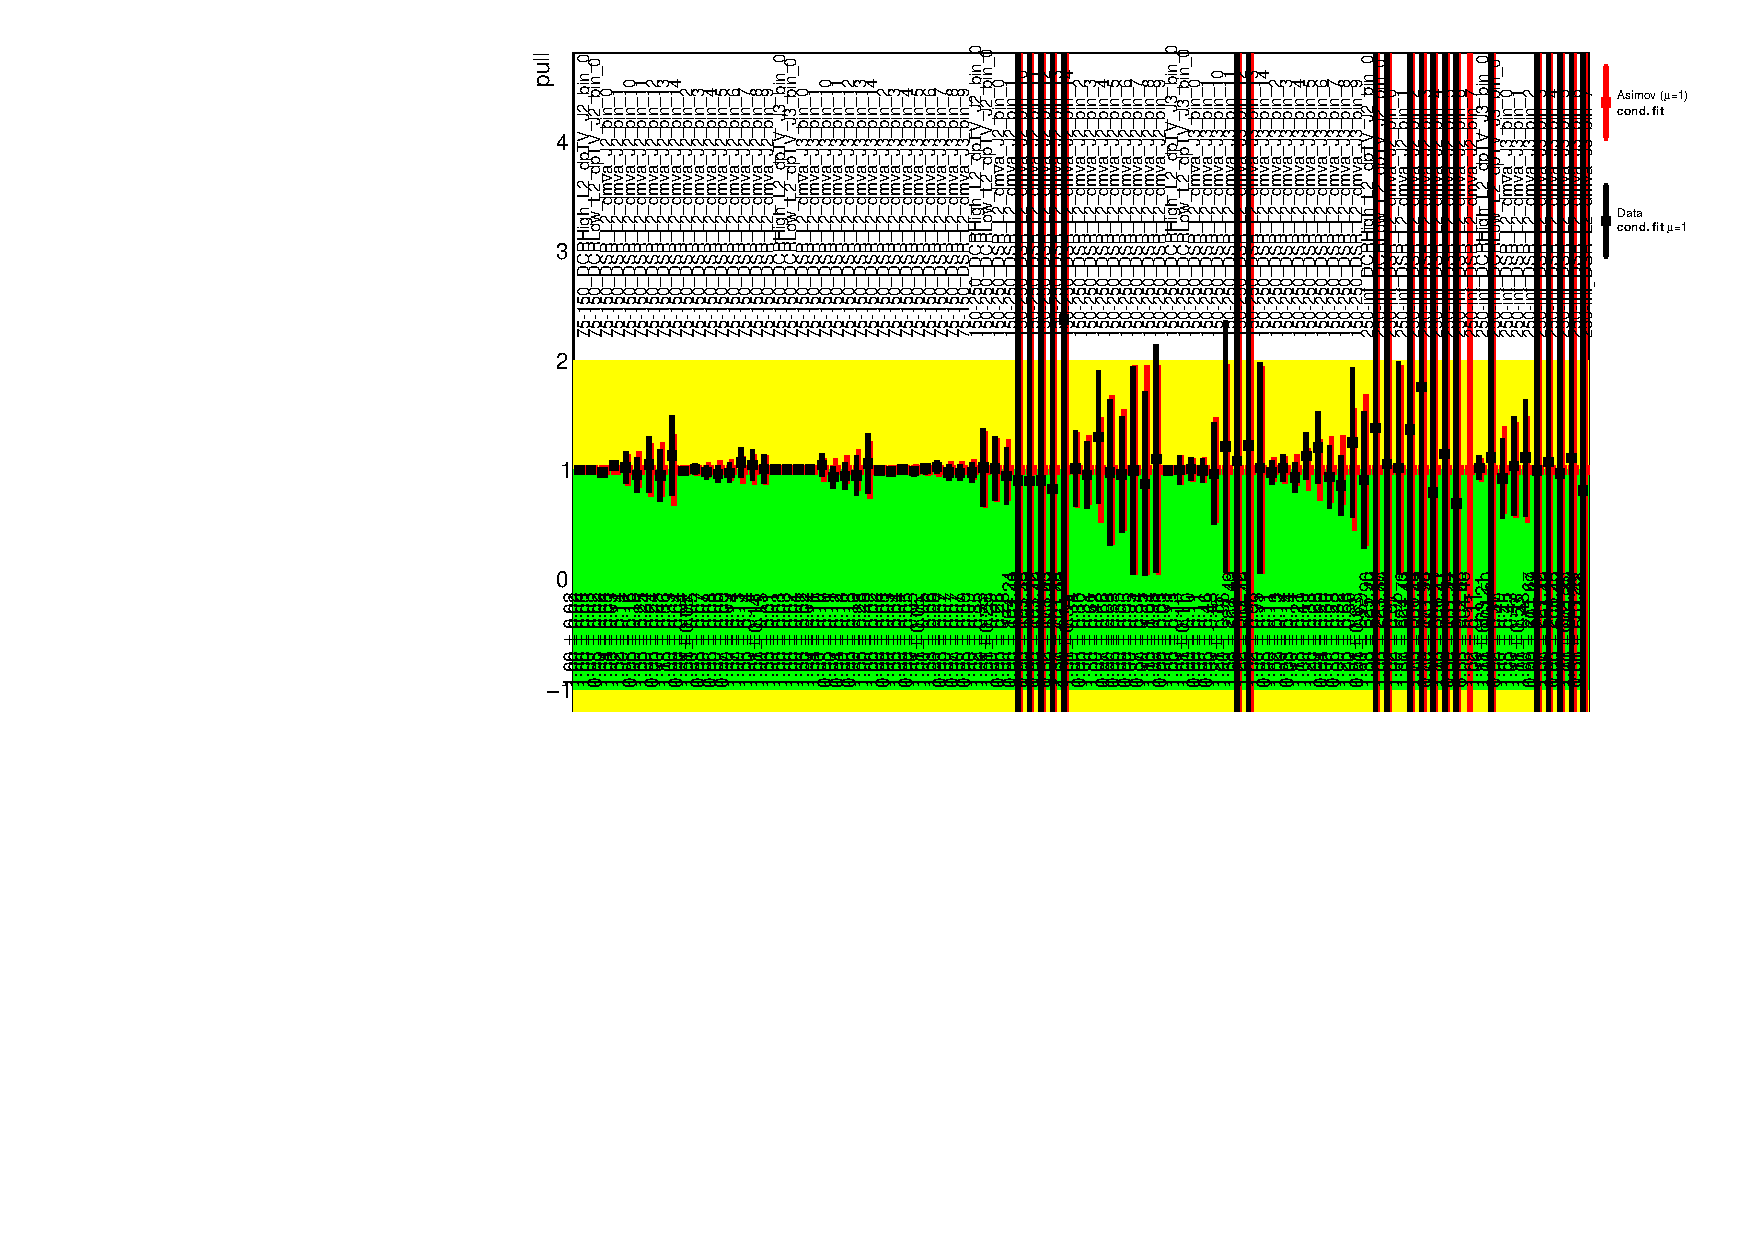
\includegraphics[width=0.49\linewidth]{final_fit_mva/pullComparisons/NP_DDttbar.pdf}
% \caption{caption}
% MC stat. nuisance parameter pulls and the free parameter scale factors
% corresponding to $0$-lepton, $1$-lepton and $2$-lepton as well as the Gamma
% parameter pulls for the data driven top template in the $2$-lepton channel
% corresponding to a conditional combined fit to the Asimov dataset (red) and an
% unconditional combined fit to the \RunTwo data (black)
% \label{fig:nppulls_012L_MVAVH_c} 
% \end{figure}
\clearpage
\section{Breakdown and Ranking of Uncertainties}
Table~\ref{tab:breakdown_012L_MVAVH} shows a breakdown of the impact of the
systematic uncertainties on the signal strength measurement.
\begin{table}[ht]
  \centering
  \begin{tabular}{lrr}
    {\bfseries POI: $\bm{\mu=\sigma/\sigma_{\text{SM}}}$} & \multicolumn{2}{r}{\bfseries Central Value = 1.02} \\ 
    \toprule
    {\bfseries Nuisance Parameter Set} & \multicolumn{2}{l}{\bfseries Impact on error}  \\
                                  & {\bfseries Signed impact} & {\bfseries Un-signed impact}  \\
    \midrule
    Total                    & +0.184 / -0.170 & $ \pm 0.177 $ \\
    \rule{0pt}{4ex}
    DataStat                 & +0.116 / -0.114 & $ \pm 0.115 $ \\
    \rule{0pt}{4ex}
    \:\: Data stat only           & +0.109 / -0.107 & $ \pm 0.108 $ \\
    \:\: Top $e\mu$ CR stat       & +0.014 / -0.014 & $ \pm 0.014 $ \\
    \:\: Floating normalizations  & +0.035 / -0.033 & $ \pm 0.034 $ \\
    \rule{0pt}{4ex}
    FullSyst                 & +0.143 / -0.126 & $ \pm 0.134 $ \\
    \rule{0pt}{4ex}
    \:\: Modelling: \VH           & +0.083 / -0.061 & $ \pm 0.072 $ \\
    \:\: Modelling: Background    & +0.068 / -0.064 & $ \pm 0.066 $ \\
    \:\:\:\: Multi Jet                & +0.004 / -0.006 & $ \pm 0.005 $ \\
    \:\:\:\: Modelling: single top    & +0.020 / -0.019 & $ \pm 0.019 $ \\
    \:\:\:\: Modelling: $t\bar{t}$    & +0.021 / -0.020 & $ \pm 0.021 $ \\
    \:\:\:\: Modelling: $W+$jets      & +0.041 / -0.038 & $ \pm 0.040 $ \\
    \:\:\:\: Modelling: $Z+$jets      & +0.032 / -0.032 & $ \pm 0.032 $ \\
    \:\:\:\: Modelling: Diboson       & +0.034 / -0.031 & $ \pm 0.033 $ \\
    \:\:\:\: MC stat                  & +0.031 / -0.030 & $ \pm 0.031 $ \\
    \rule{0pt}{4ex}
    \:\: Experimental Syst        & +0.079 / -0.069 & $ \pm 0.074 $ \\
    \:\:\:\: Detector: lepton         & +0.004 / -0.005 & $ \pm 0.004 $ \\
    \:\:\:\: Detector: MET            & +0.015 / -0.014 & $ \pm 0.015 $ \\
    \:\:\:\: Detector: JET            & +0.048 / -0.038 & $ \pm 0.043 $ \\
    \:\:\:\: Detector: FTAG (b-jet)   & +0.047 / -0.042 & $ \pm 0.045 $ \\
    \:\:\:\: Detector: FTAG (c-jet)   & +0.037 / -0.033 & $ \pm 0.035 $ \\
    \:\:\:\: Detector: FTAG (l-jet)   & +0.009 / -0.009 & $ \pm 0.009 $ \\
    \:\:\:\: Detector: FTAG (extrap)  & +0.000 / -0.000 & $ \pm 0.000 $ \\
    \:\:\:\: Detector: PU             & +0.002 / -0.003 & $ \pm 0.003 $ \\
    \:\:\:\: Luminosity               & +0.019 / -0.013 & $ \pm 0.016 $ \\
    \bottomrule
  \end{tabular}
\caption{This table shows the impact of systematic uncertainties on the signal
  strength $\mu$ broken down into categories or nuisance parameter sets. Some
  sets are further broken down into smaller categories indicated by nested
  indentation.}
\label{tab:breakdown_012L_MVAVH}
\end{table}
It can be seen that the total statistical uncertainty (DataStat) has a smaller
impact that the uncertainties due to modelling and experimental sources
(FullSyst). Considering the systematic uncertainties, those coming from
experimental sources have a greater impact than those coming from the modelling
of the signal, which in turn have a greater impact  that those coming from the
modelling of the background. Further scrutiny of uncertainties on the signal
strength comes in the form of the ranking shown in
figure~\ref{fig:Rank_012L_MVAVH}.
\begin{figure}[ht]
  \centering
  %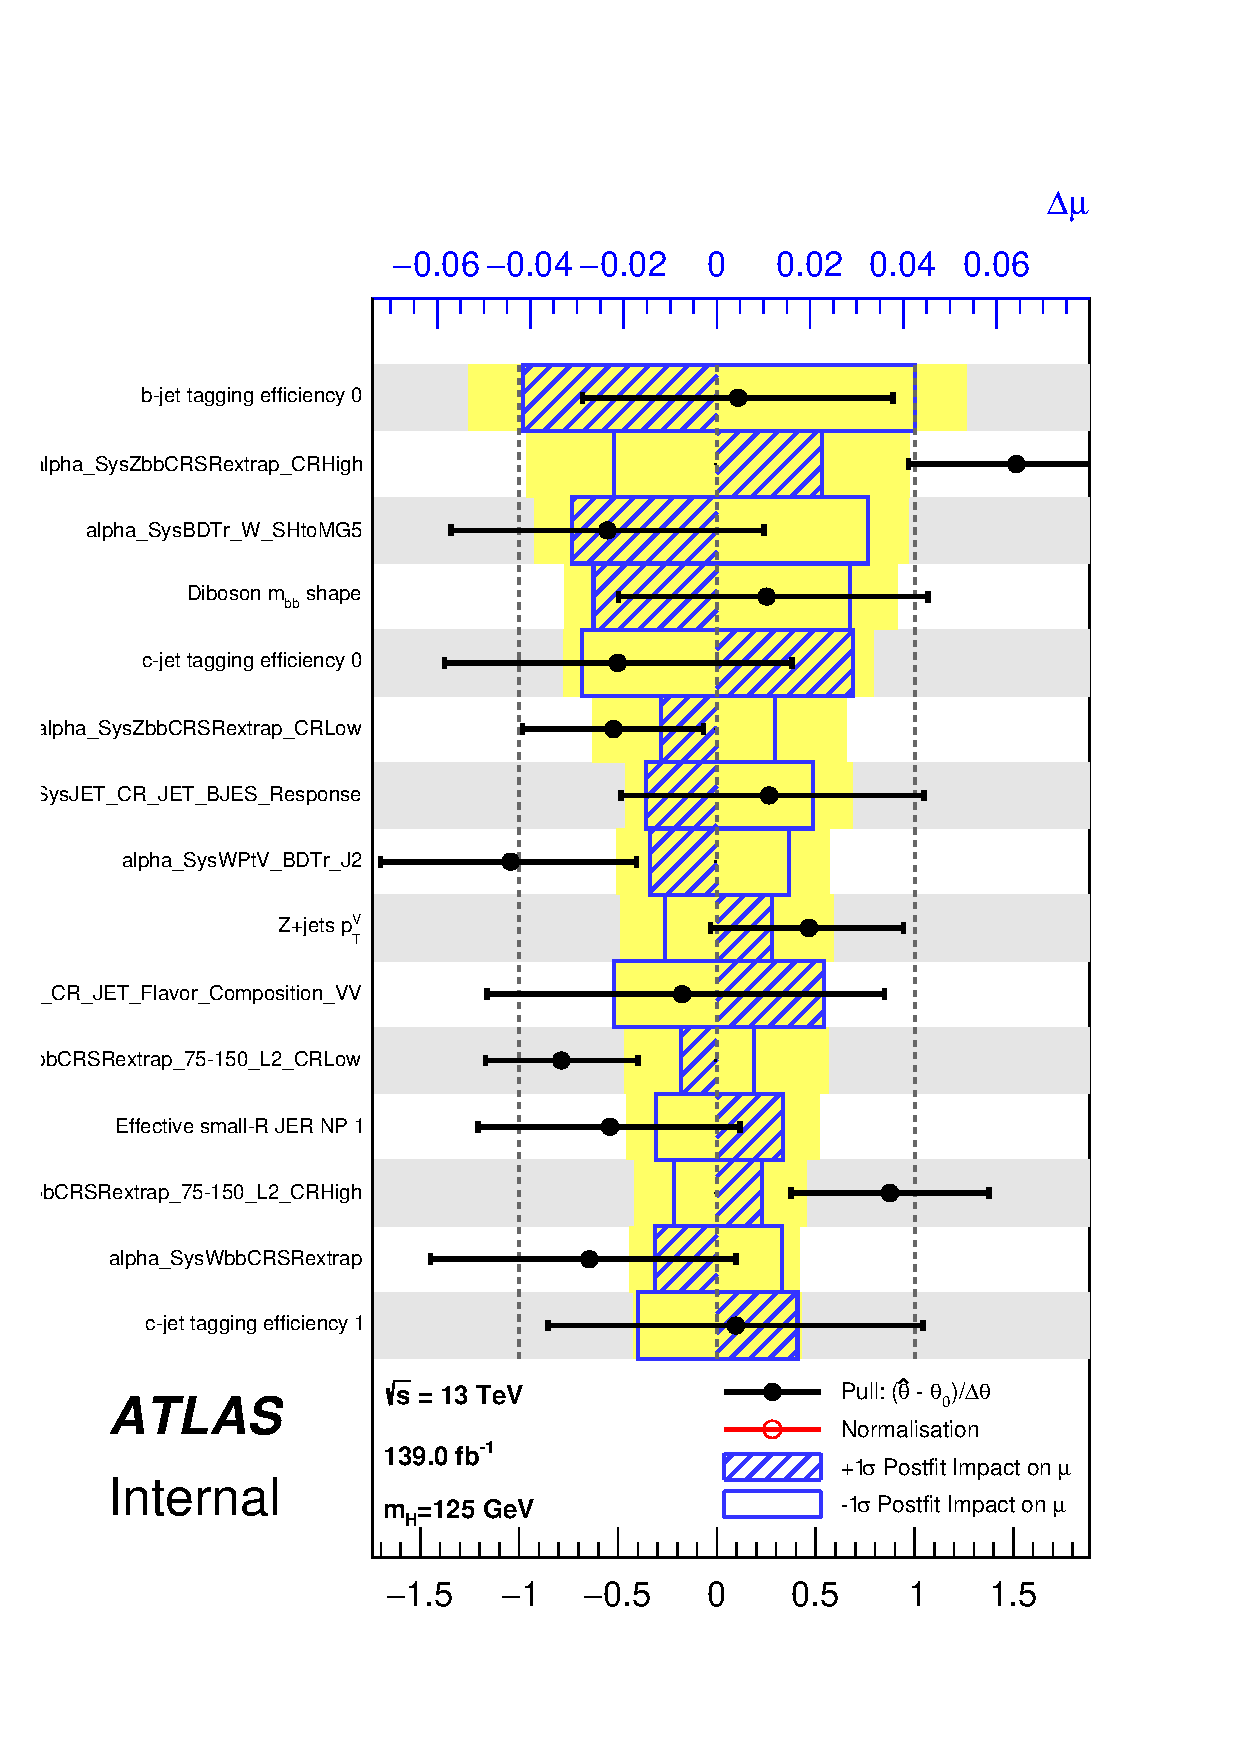
\includegraphics[width=0.49\linewidth]{final_fit_mva/ranking/pulls_SigXsecOverSM_prefit_125_NOSignalUnc.pdf} \\
  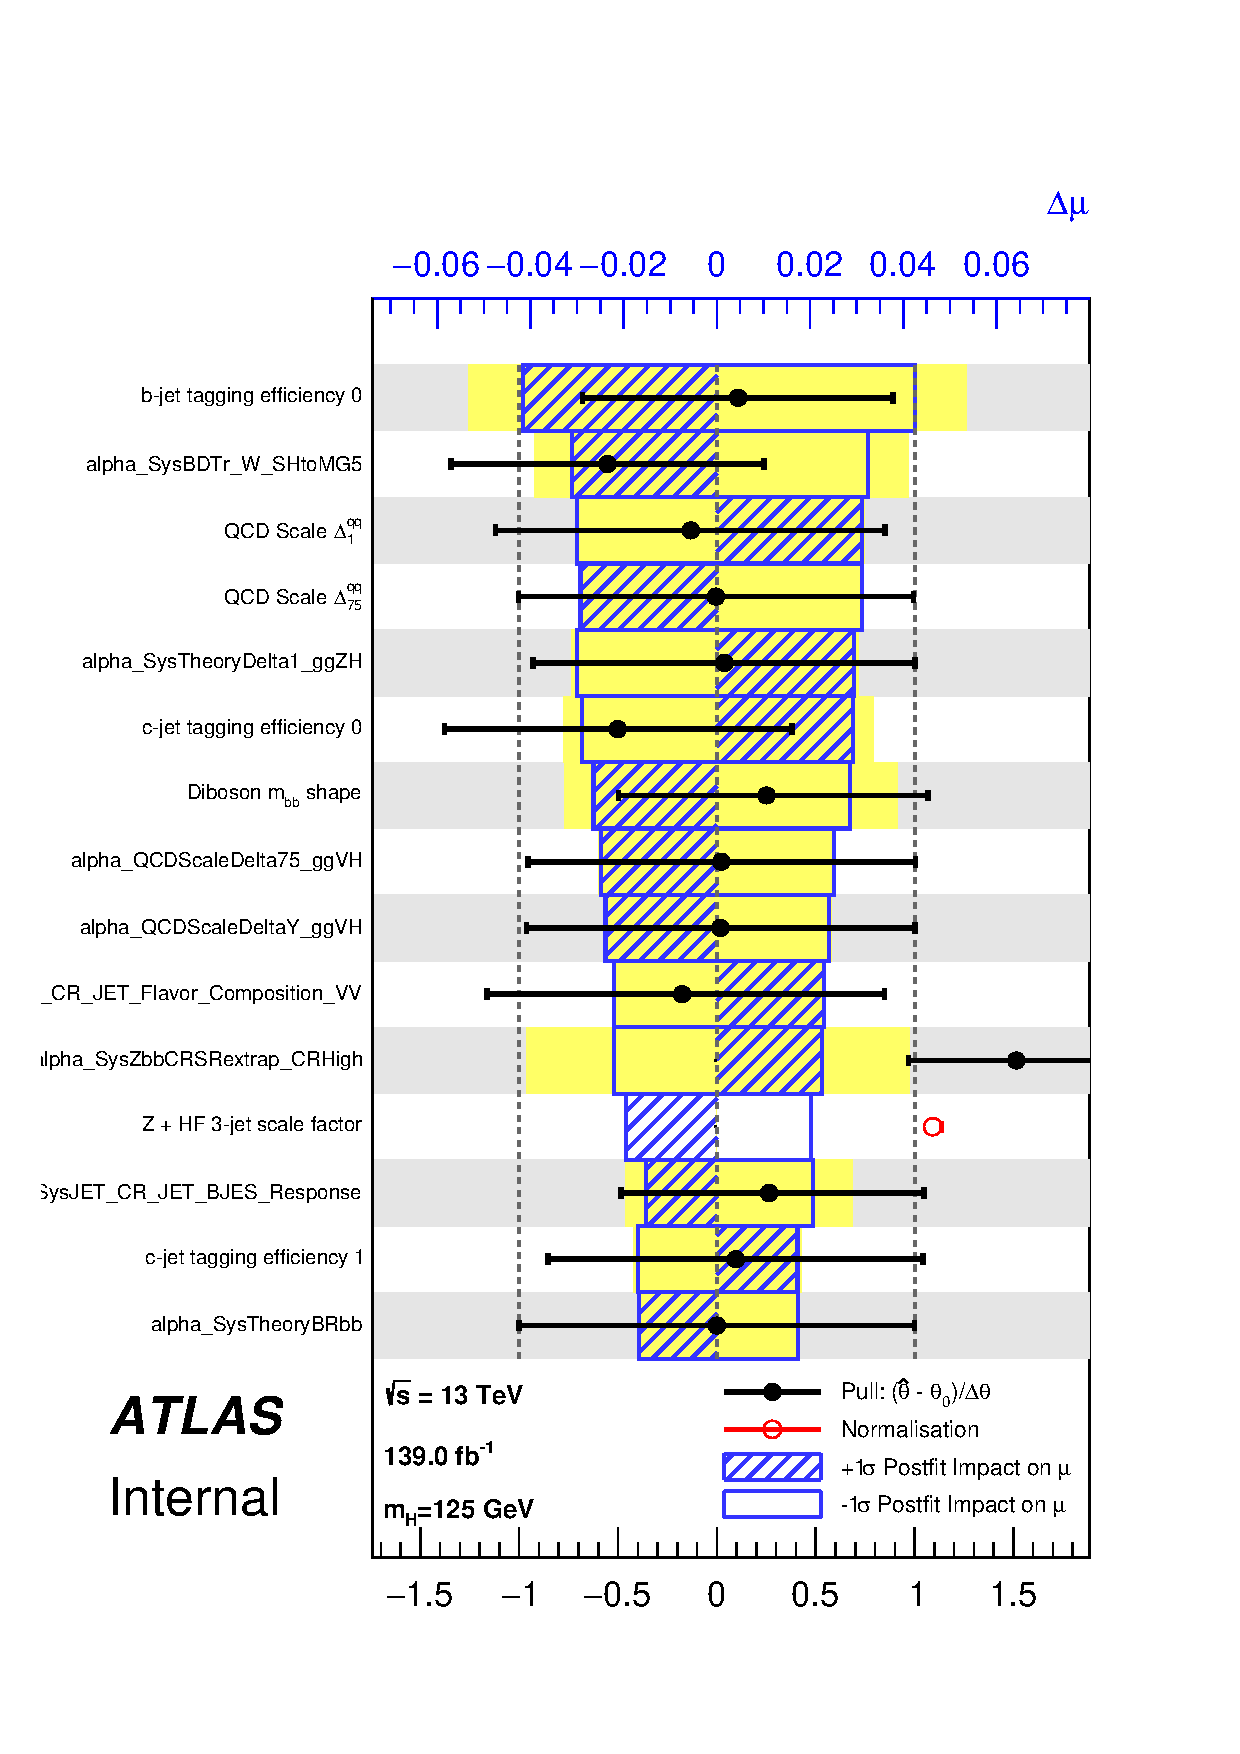
\includegraphics[width=0.75\linewidth]{final_fit_mva/ranking/pulls_SigXsecOverSM_125_SignalUnc.pdf}
  \\
  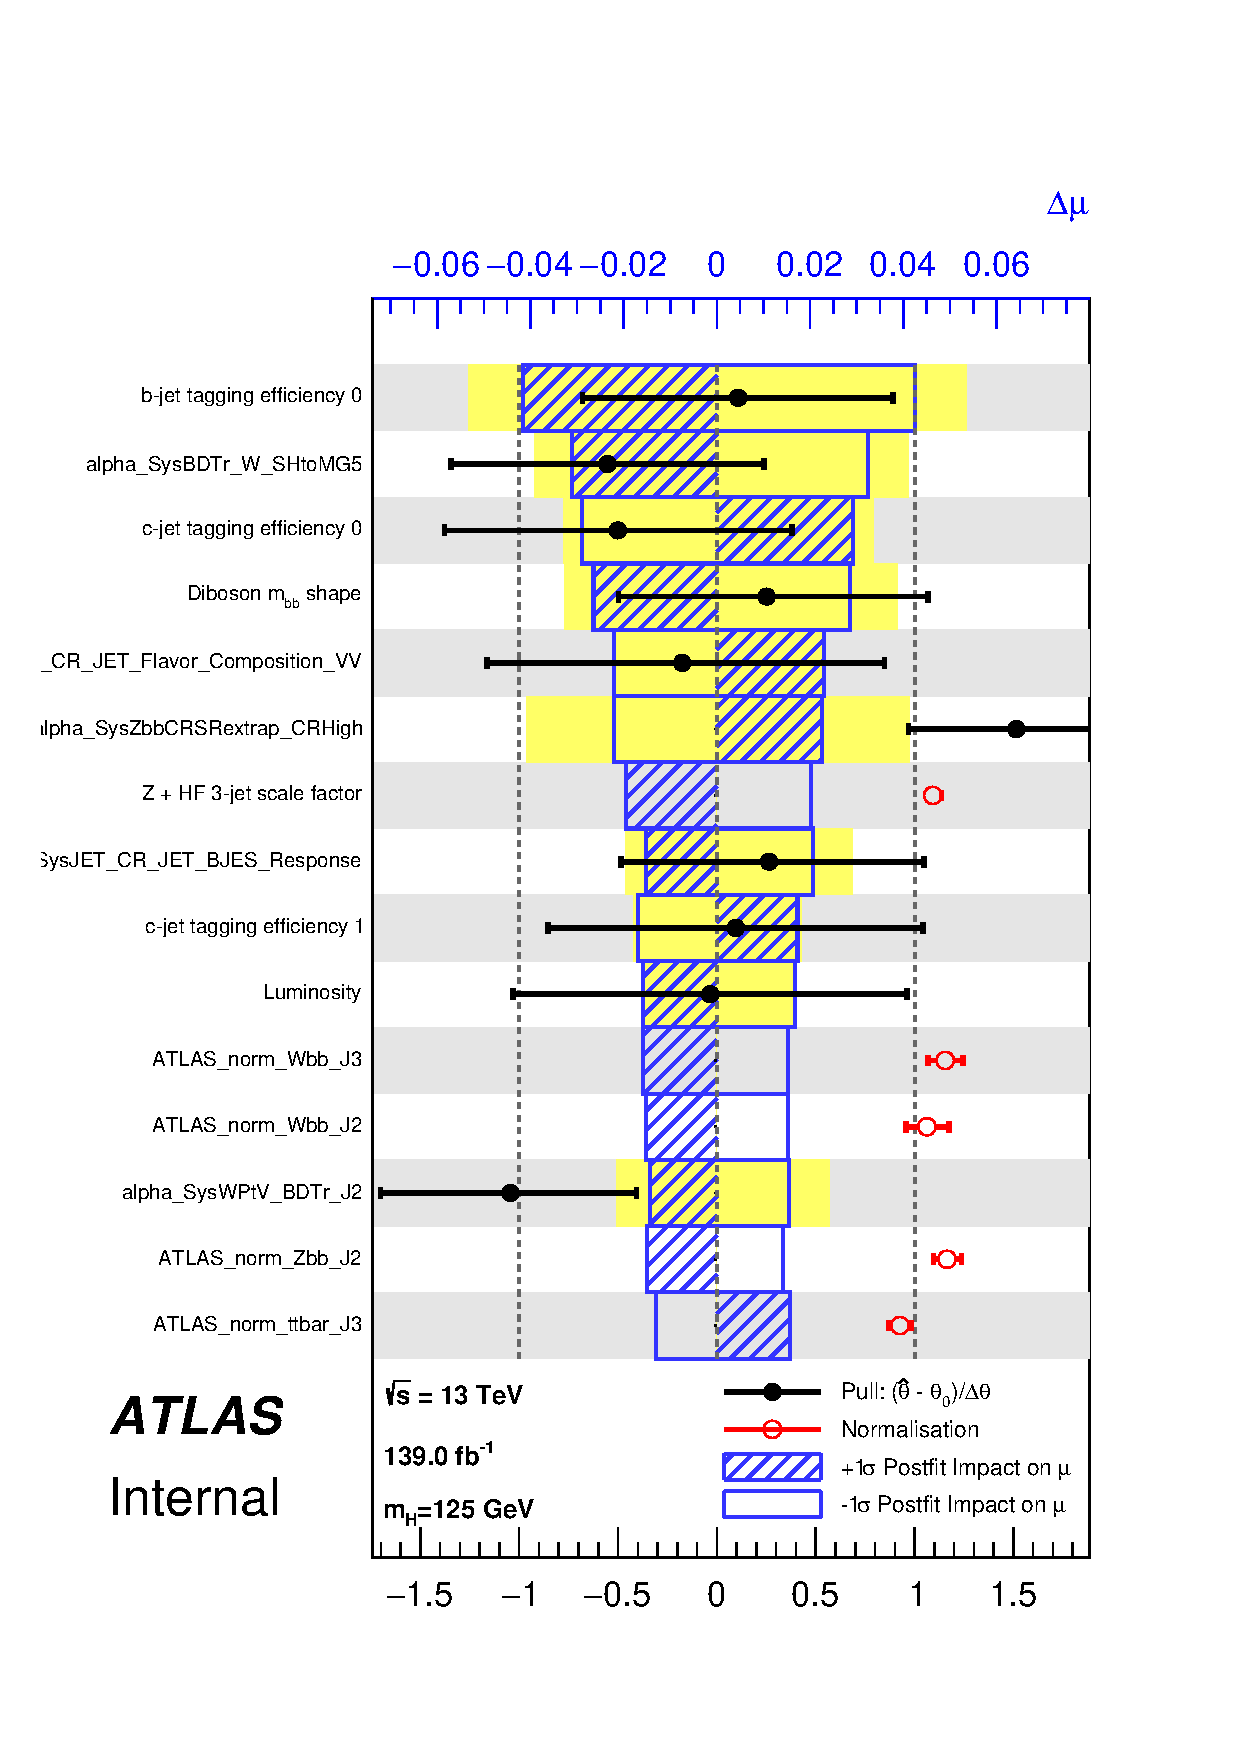
\includegraphics[width=0.75\linewidth]{final_fit_mva/ranking/pulls_SigXsecOverSM_125_NOSignalUnc.pdf}
  \caption{The top 15 nuisance parameters are shown ranked based on their impact
  on the \VHbb\ signal strength $\mu$ as determined by the combined
  unconditional fit to data. Two scenarios the post-fit rankings including and
  excluding signal uncertainties on the left and right respectively.}
  \label{fig:Rank_012L_MVAVH}
\end{figure}
It can be seen in the post-fit ranking that the top 15 is dominated by
uncertainties on the signal. The post-fit ranking which omits signal
uncertainties is largely dominated by flavour tagging uncertainties and scale
factors for normalisation and acceptance between analysis regions. The highest
ranked uncertainty in both cases is the $b$-tagging efficiency, this is
unsurprising as $b$-tagging plays a crucial role in the analysis selection.

Notably the $Z+$jets shape uncertainties do not appear in the top 15 sources of
uncertainty, naively this is unexpected as the background dominates in a
sensitive channel of the analysis. Improvements to the separation of the
$Z+$jets background and the signal in the analysis MVA due to the inclusion of
the $Z+$jets polarisation information is likely the reason for the shape
uncertainties not being as impactful as might be expected. 
\clearpage

\section{Post-fit Data Versus Predictions}
Figures~\ref{fig:0lep2jet-postfit}, \ref{fig:0lep3jet-postfit},
\ref{fig:1lep2jet-postfit}, \ref{fig:1lep3jet-postfit},
\ref{fig:2lep2jet-postfit}, \ref{fig:2lep3pjet-postfit} show the post-fit data
versus prediction comparisons for each of the analysis channel, jet multiplicity
combinations. Each figure shows the individual analysis regions based on
$\Delta R(b, b)$ region and $p_{\mathrm{T}}^V$ bin. Across the board good
agreement between the data and prediction can be seen, supporting the fact that
our uncertainty model covers all of the differences between the two datasets and
the also supporting the background plus signal hypothesis.
\begin{figure}
  \centering
  \begin{tabular}{cc}
    % top row
    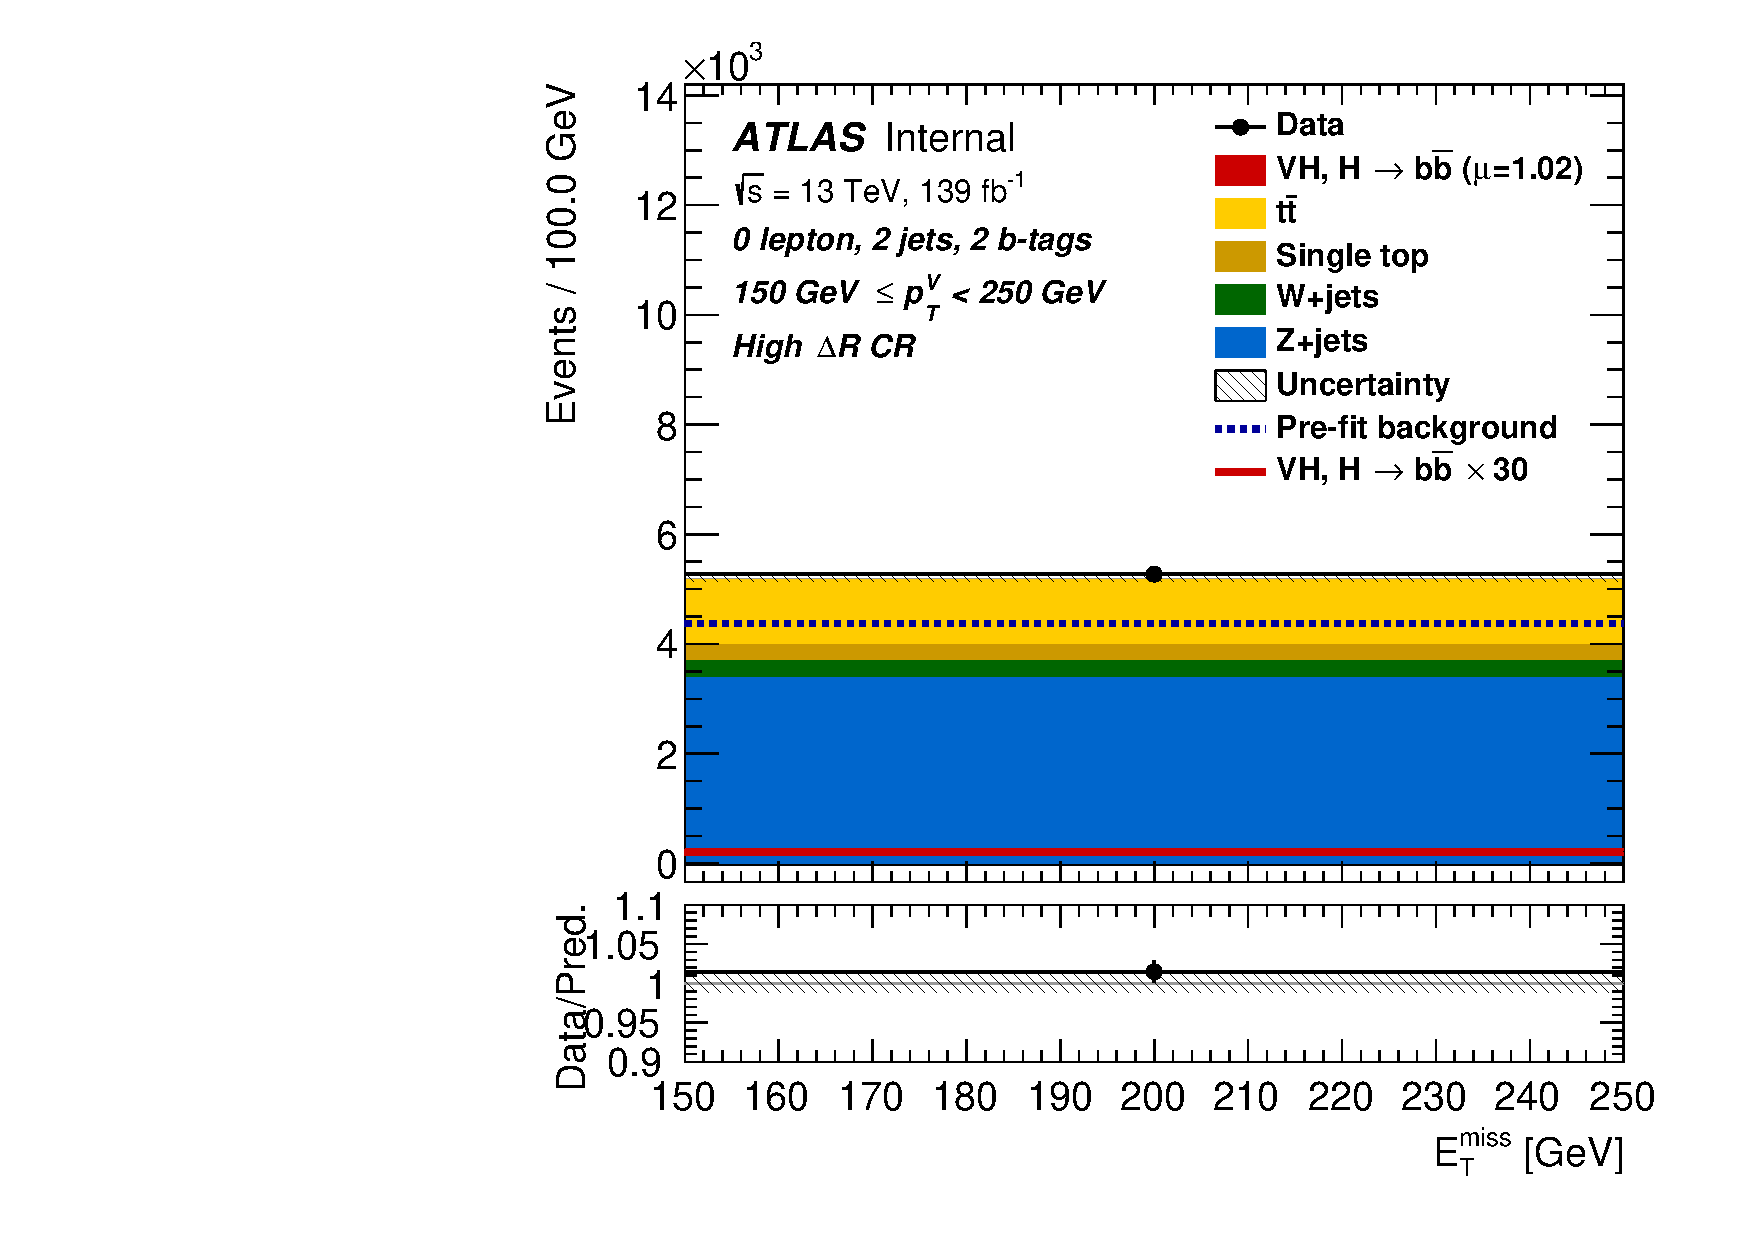
\includegraphics[width=.49\textwidth]{final_fit_mva/postfit/Region_BMax250_BMin150_Y6051_DCRHigh_T2_L0_distMET_J2_GlobalFit_unconditionnal_mu1}%
    & 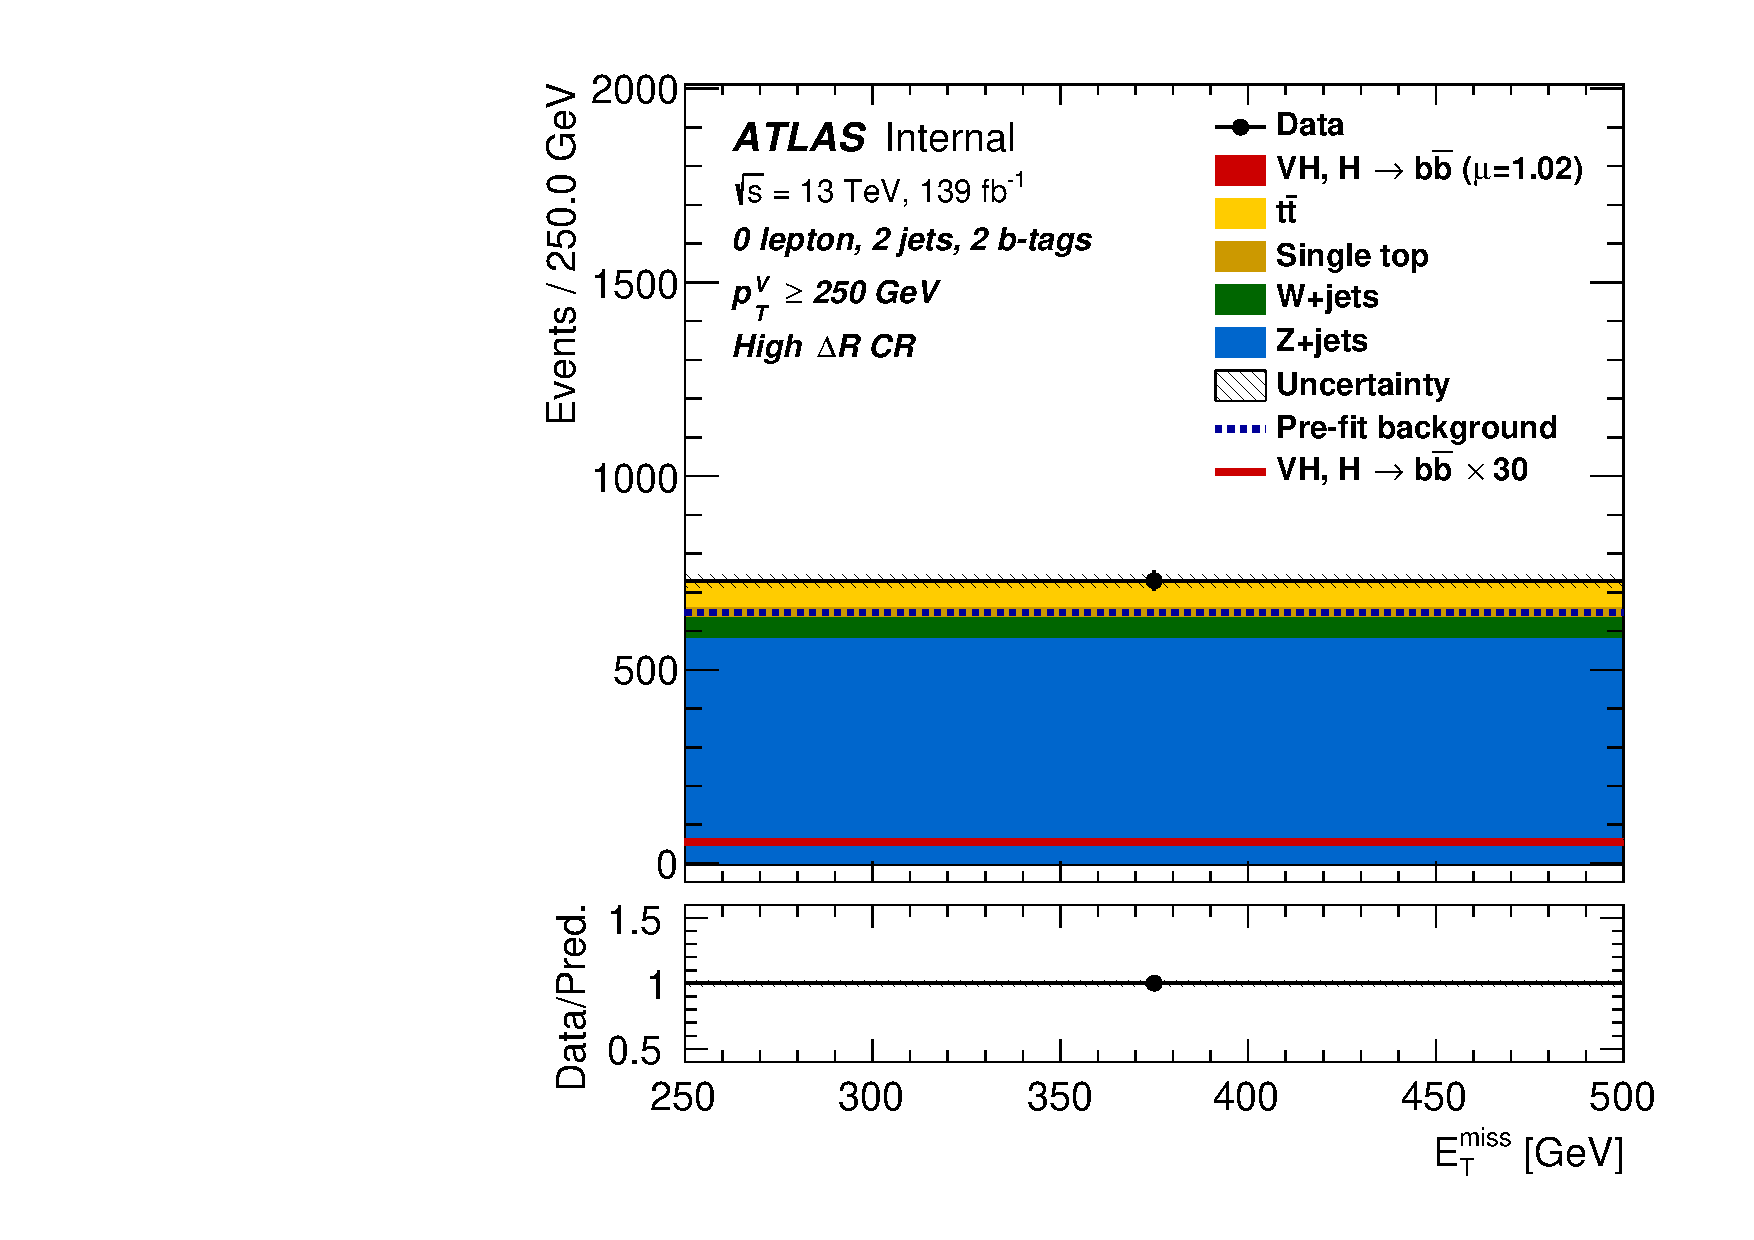
\includegraphics[width=.49\textwidth]{final_fit_mva/postfit/Region_BMin250_Y6051_DCRHigh_T2_L0_distMET_J2_GlobalFit_unconditionnal_mu1} \\

    % middle row
    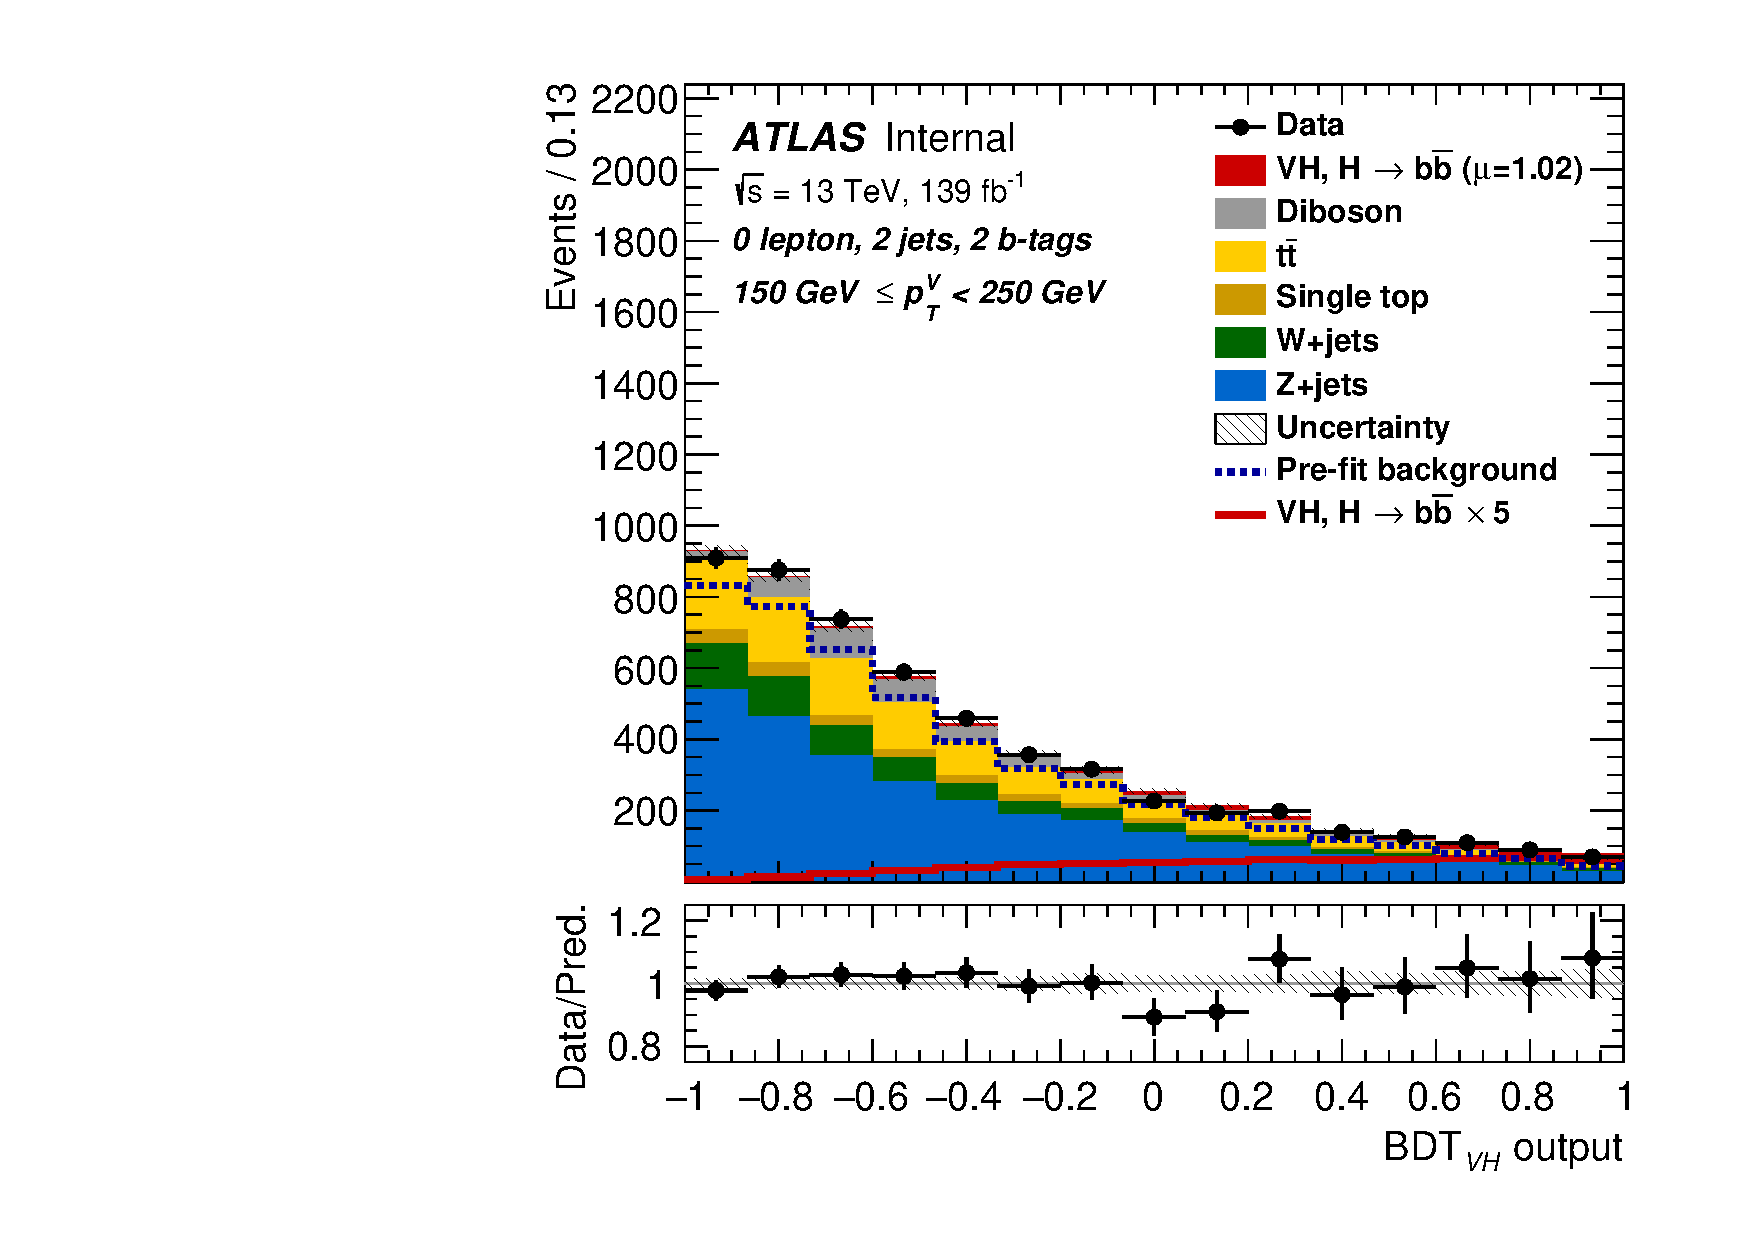
\includegraphics[width=.49\textwidth]{final_fit_mva/postfit/Region_BMax250_BMin150_Y6051_DSR_T2_L0_distmva_J2_GlobalFit_unconditionnal_mu1}%
    & 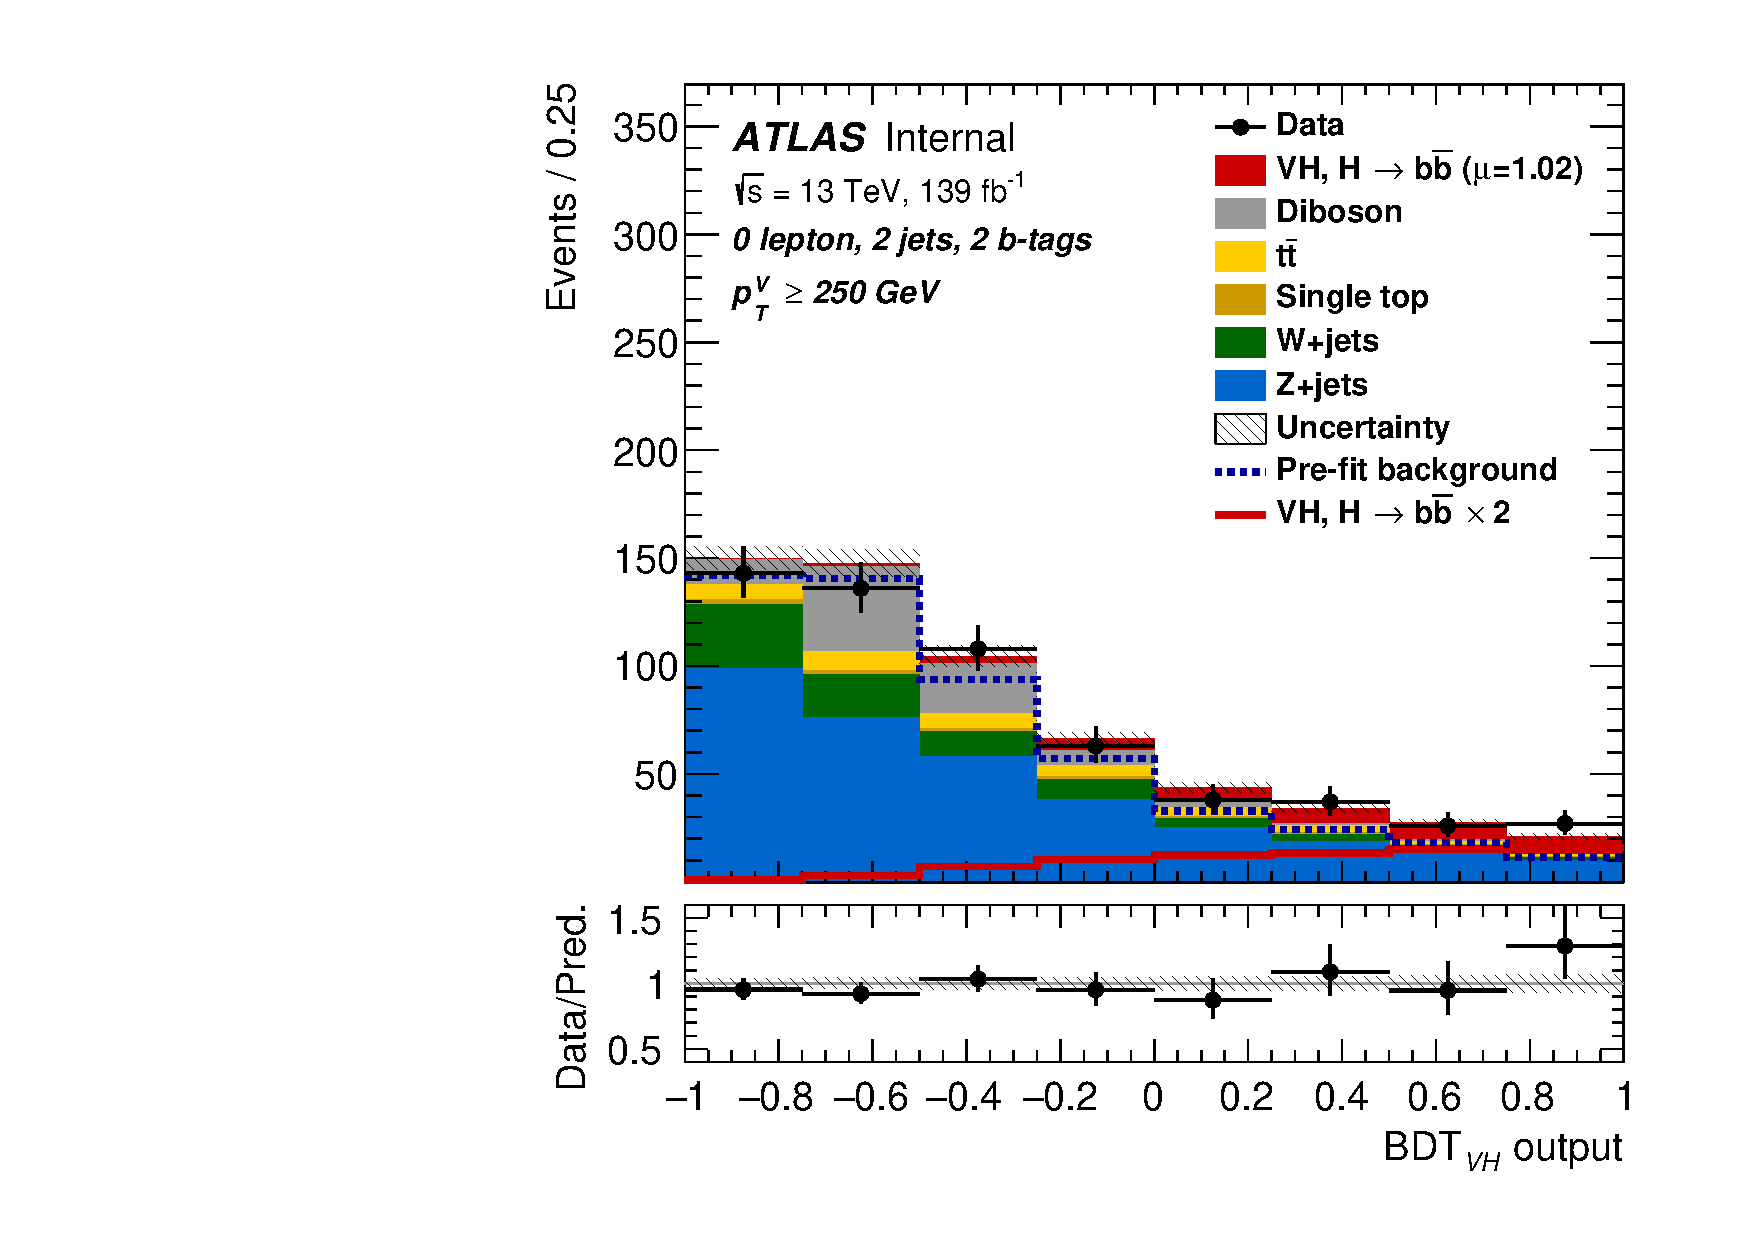
\includegraphics[width=.49\textwidth]{final_fit_mva/postfit/Region_BMin250_Y6051_DSR_T2_L0_distmva_J2_GlobalFit_unconditionnal_mu1} \\

    % bottom row
    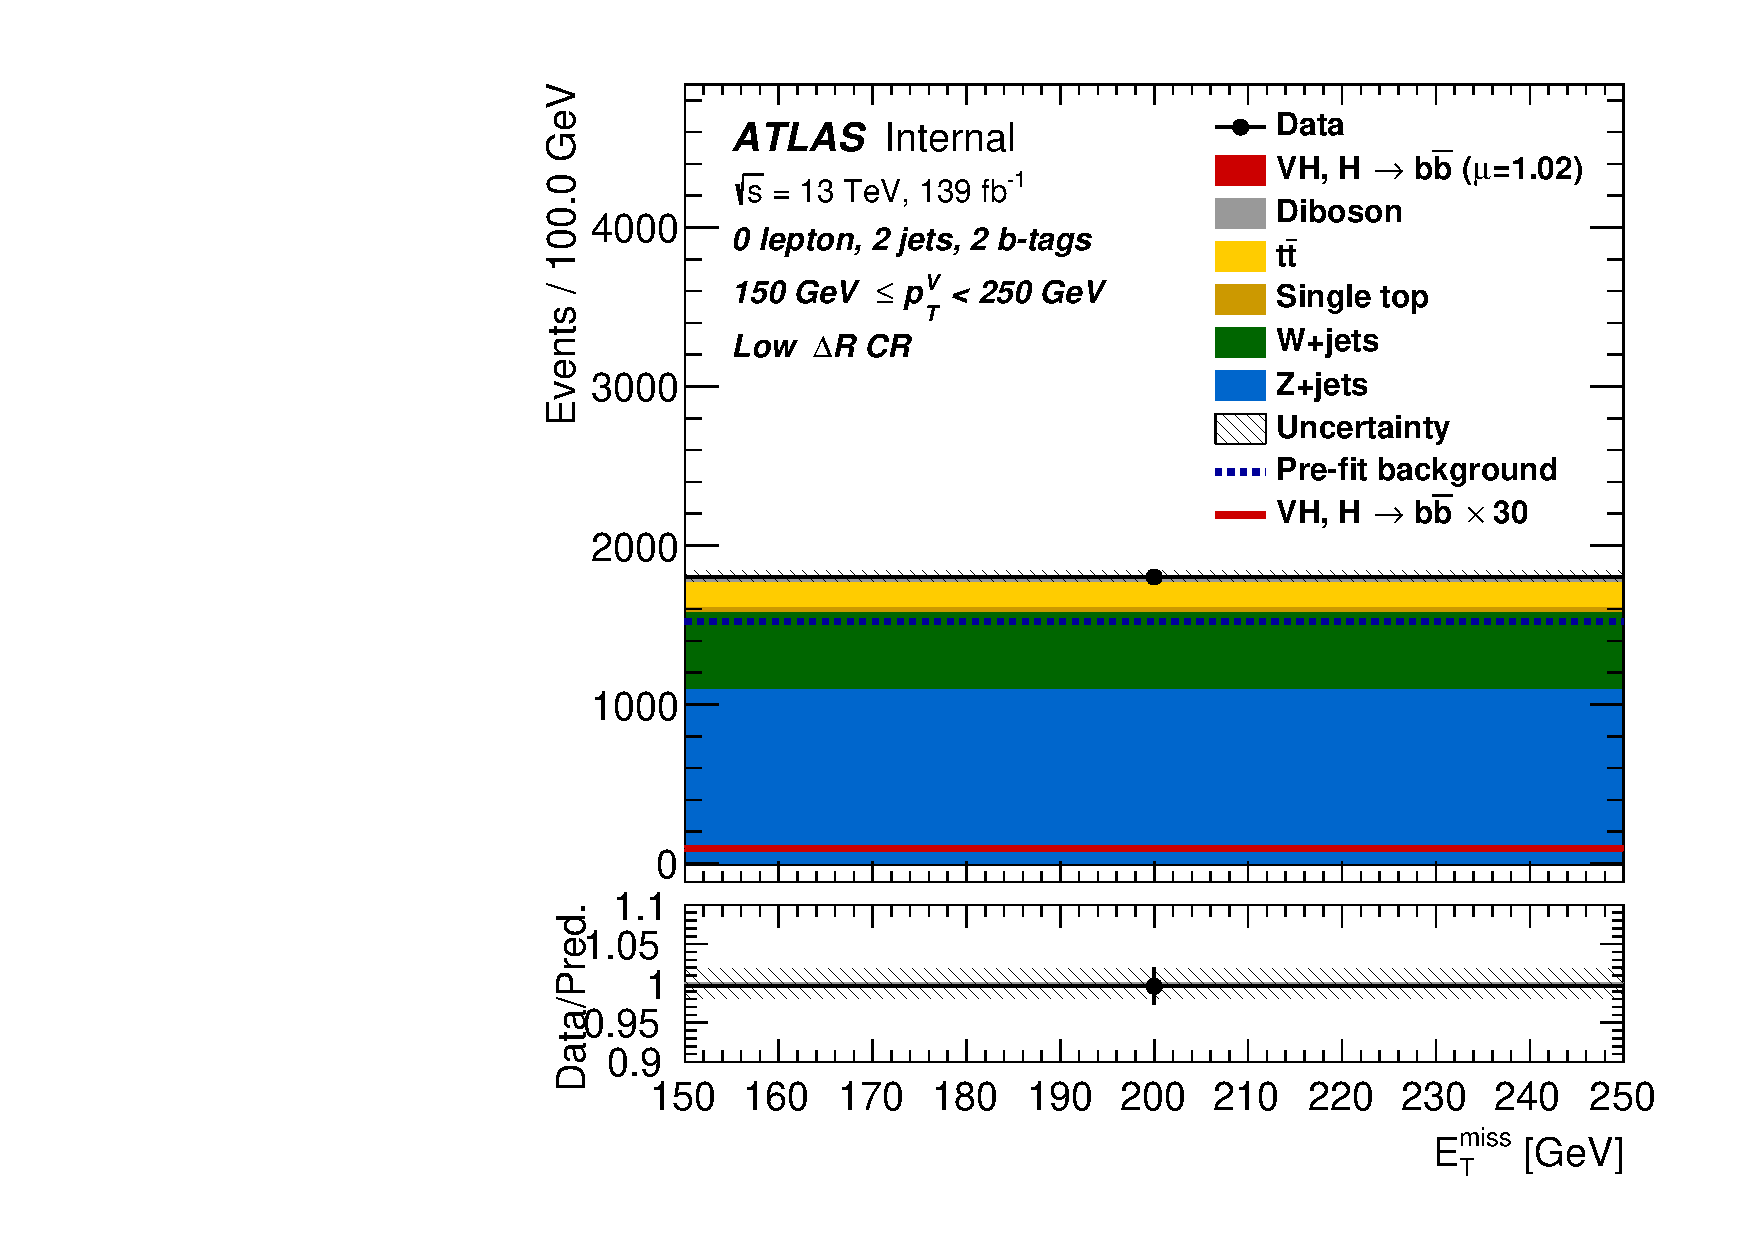
\includegraphics[width=.49\textwidth]{final_fit_mva/postfit/Region_BMax250_BMin150_Y6051_DCRLow_T2_L0_distMET_J2_GlobalFit_unconditionnal_mu1}%
    & 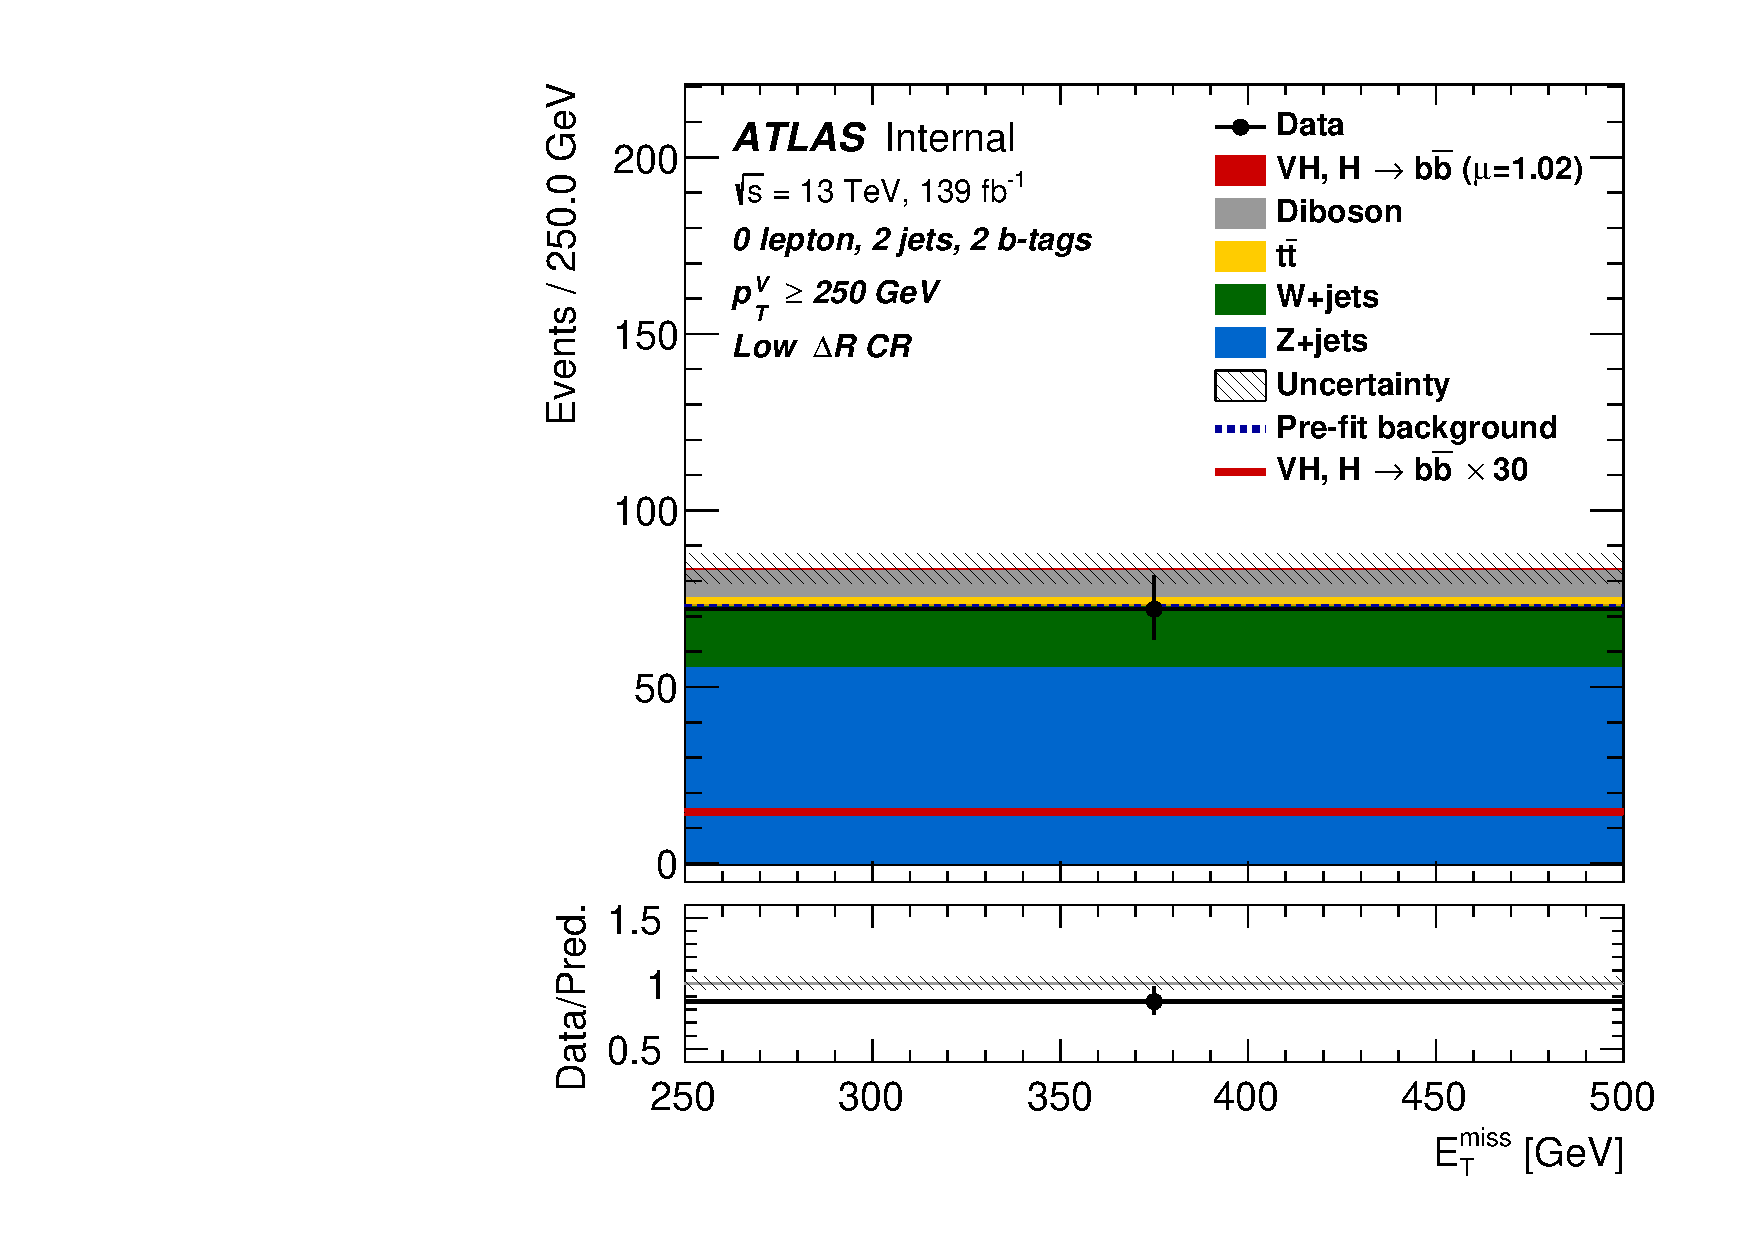
\includegraphics[width=.49\textwidth]{final_fit_mva/postfit/Region_BMin250_Y6051_DCRLow_T2_L0_distMET_J2_GlobalFit_unconditionnal_mu1} \\
  \end{tabular}
  \caption{Post-fit distributions in the 0--lepton 2--jet channel.}
  \label{fig:0lep2jet-postfit}
\end{figure}
\begin{figure}
  \centering
  \begin{tabular}{cc}
    % top row
    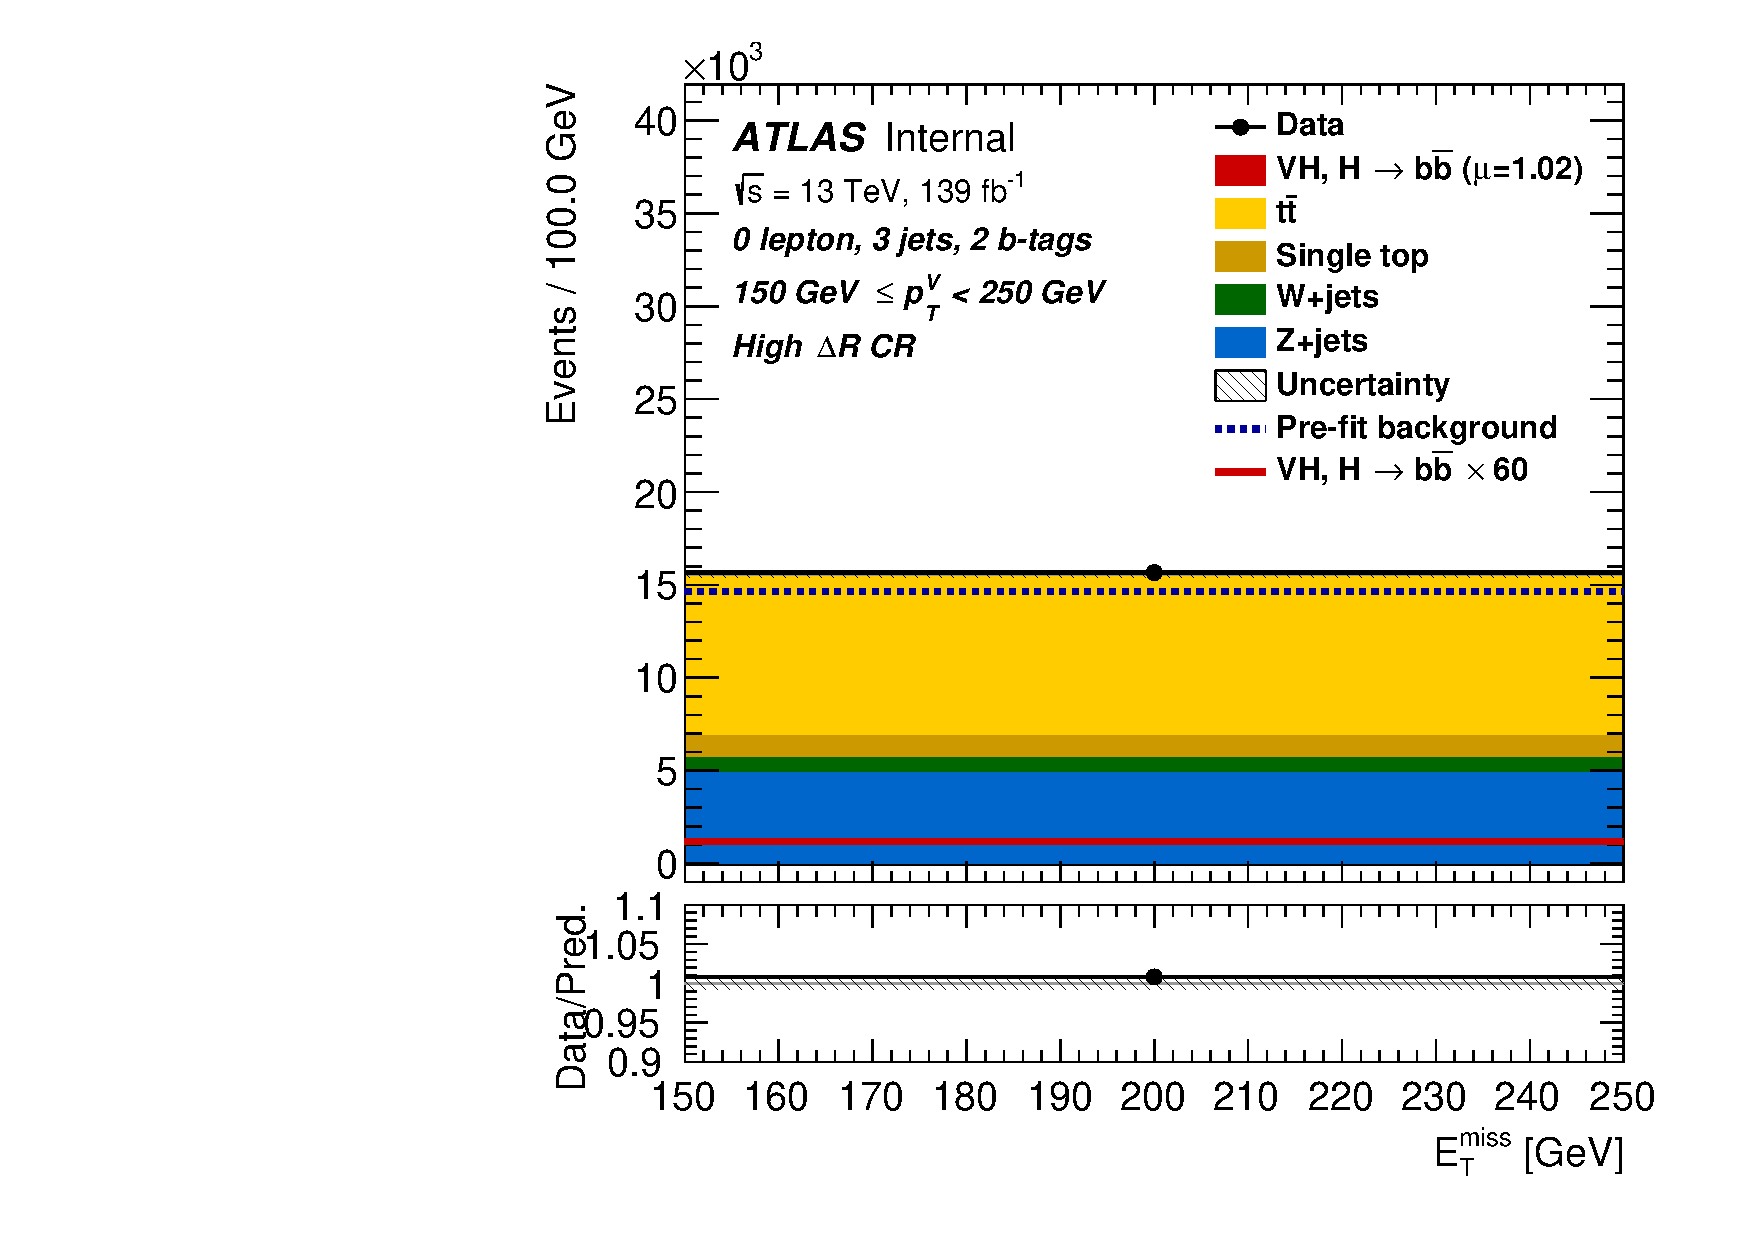
\includegraphics[width=.3\textwidth]{final_fit_mva/postfit/Region_BMax250_BMin150_Y6051_DCRHigh_T2_L0_distMET_J3_GlobalFit_unconditionnal_mu1}%
    & 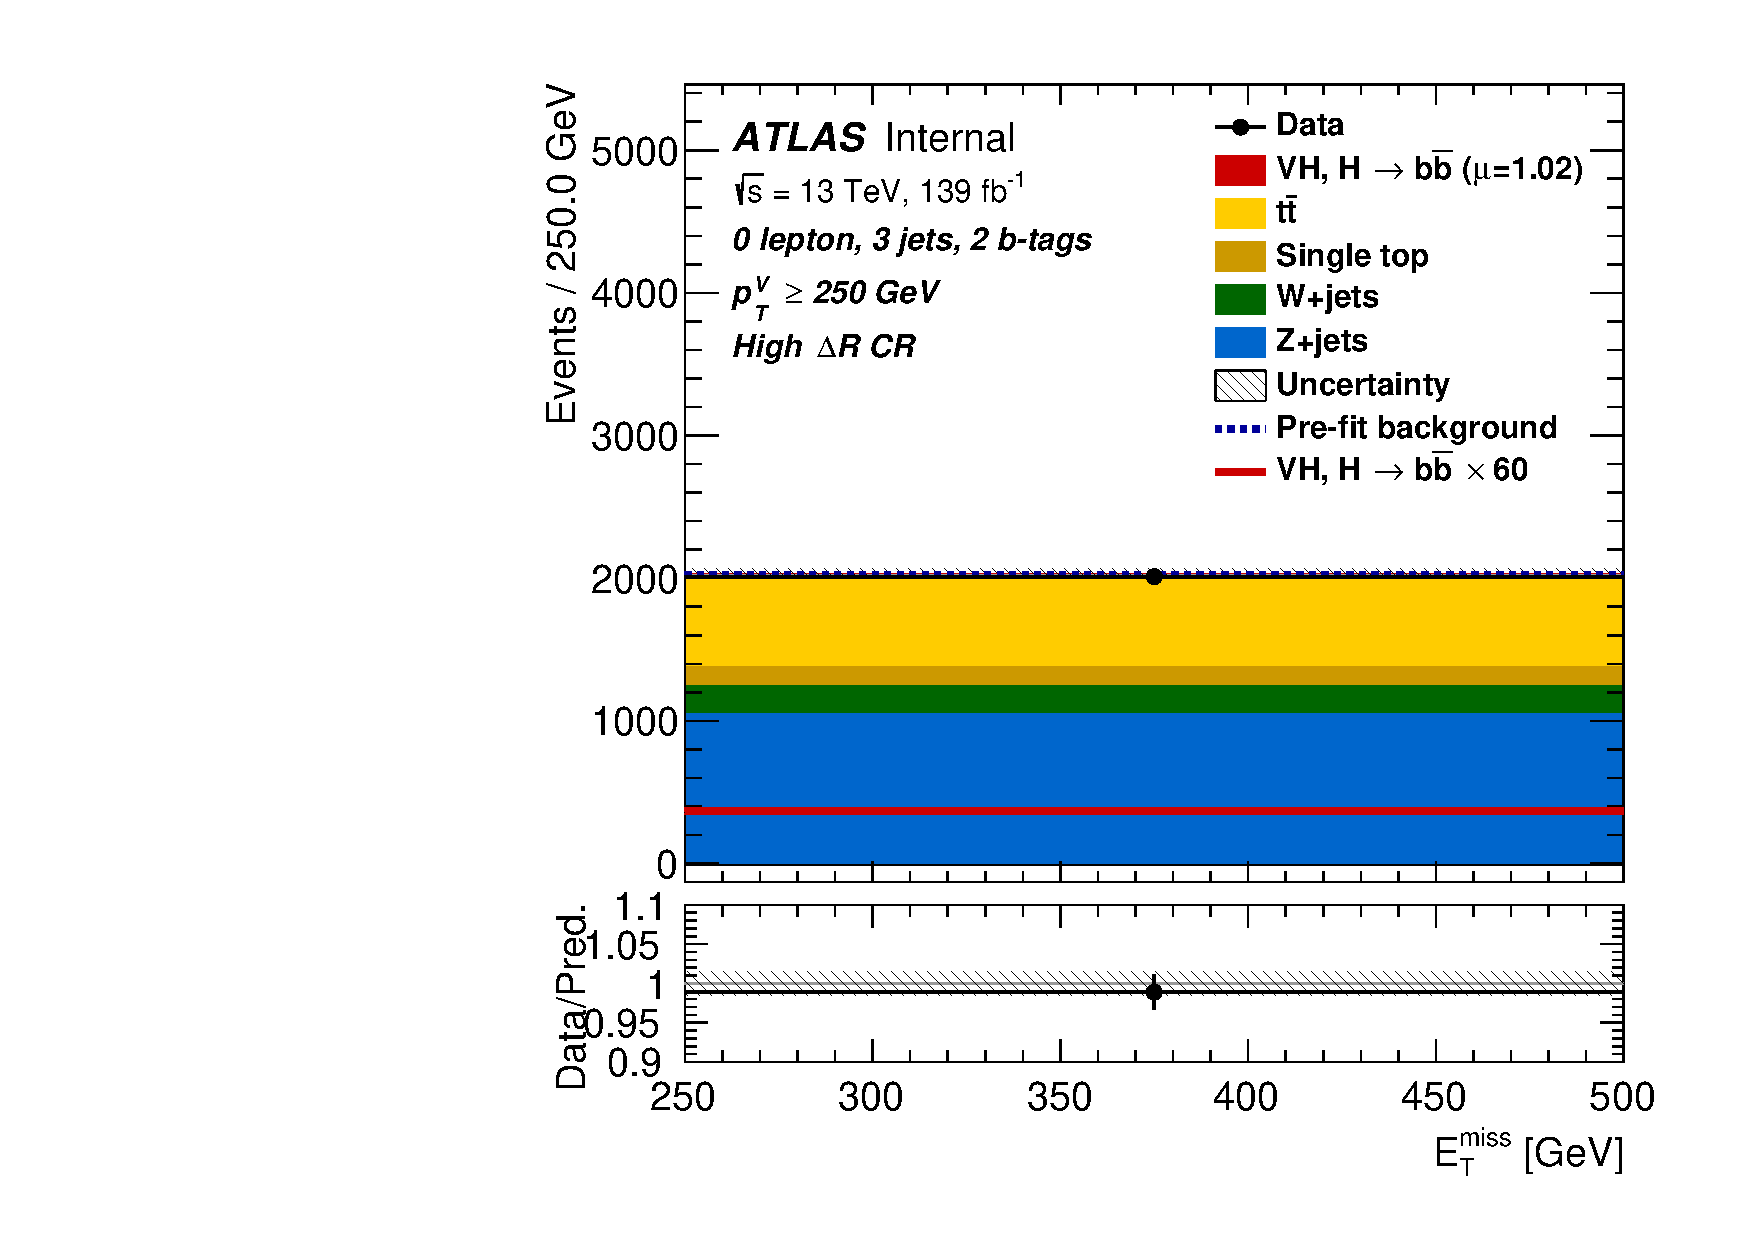
\includegraphics[width=.3\textwidth]{final_fit_mva/postfit/Region_BMin250_Y6051_DCRHigh_T2_L0_distMET_J3_GlobalFit_unconditionnal_mu1} \\

    % middle row
    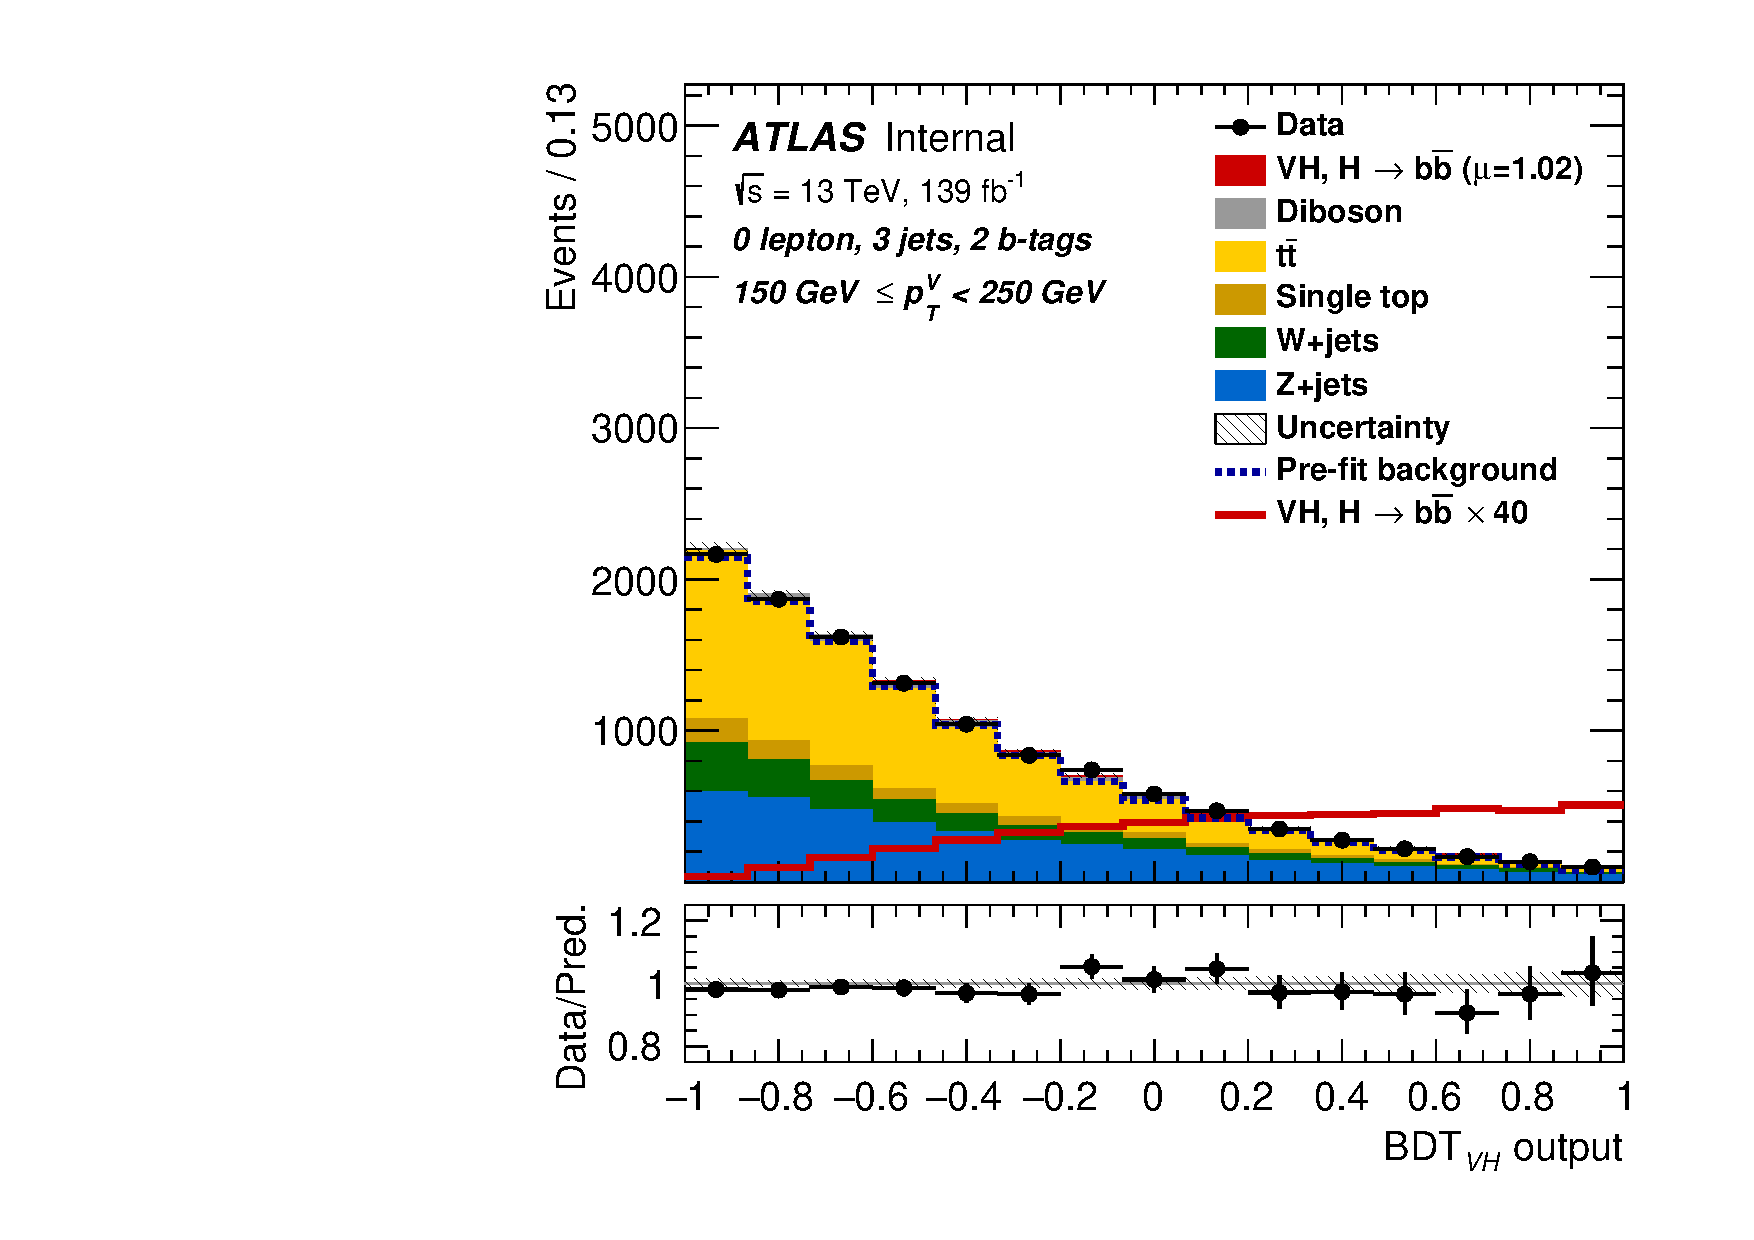
\includegraphics[width=.3\textwidth]{final_fit_mva/postfit/Region_BMax250_BMin150_Y6051_DSR_T2_L0_distmva_J3_GlobalFit_unconditionnal_mu1}%
    & 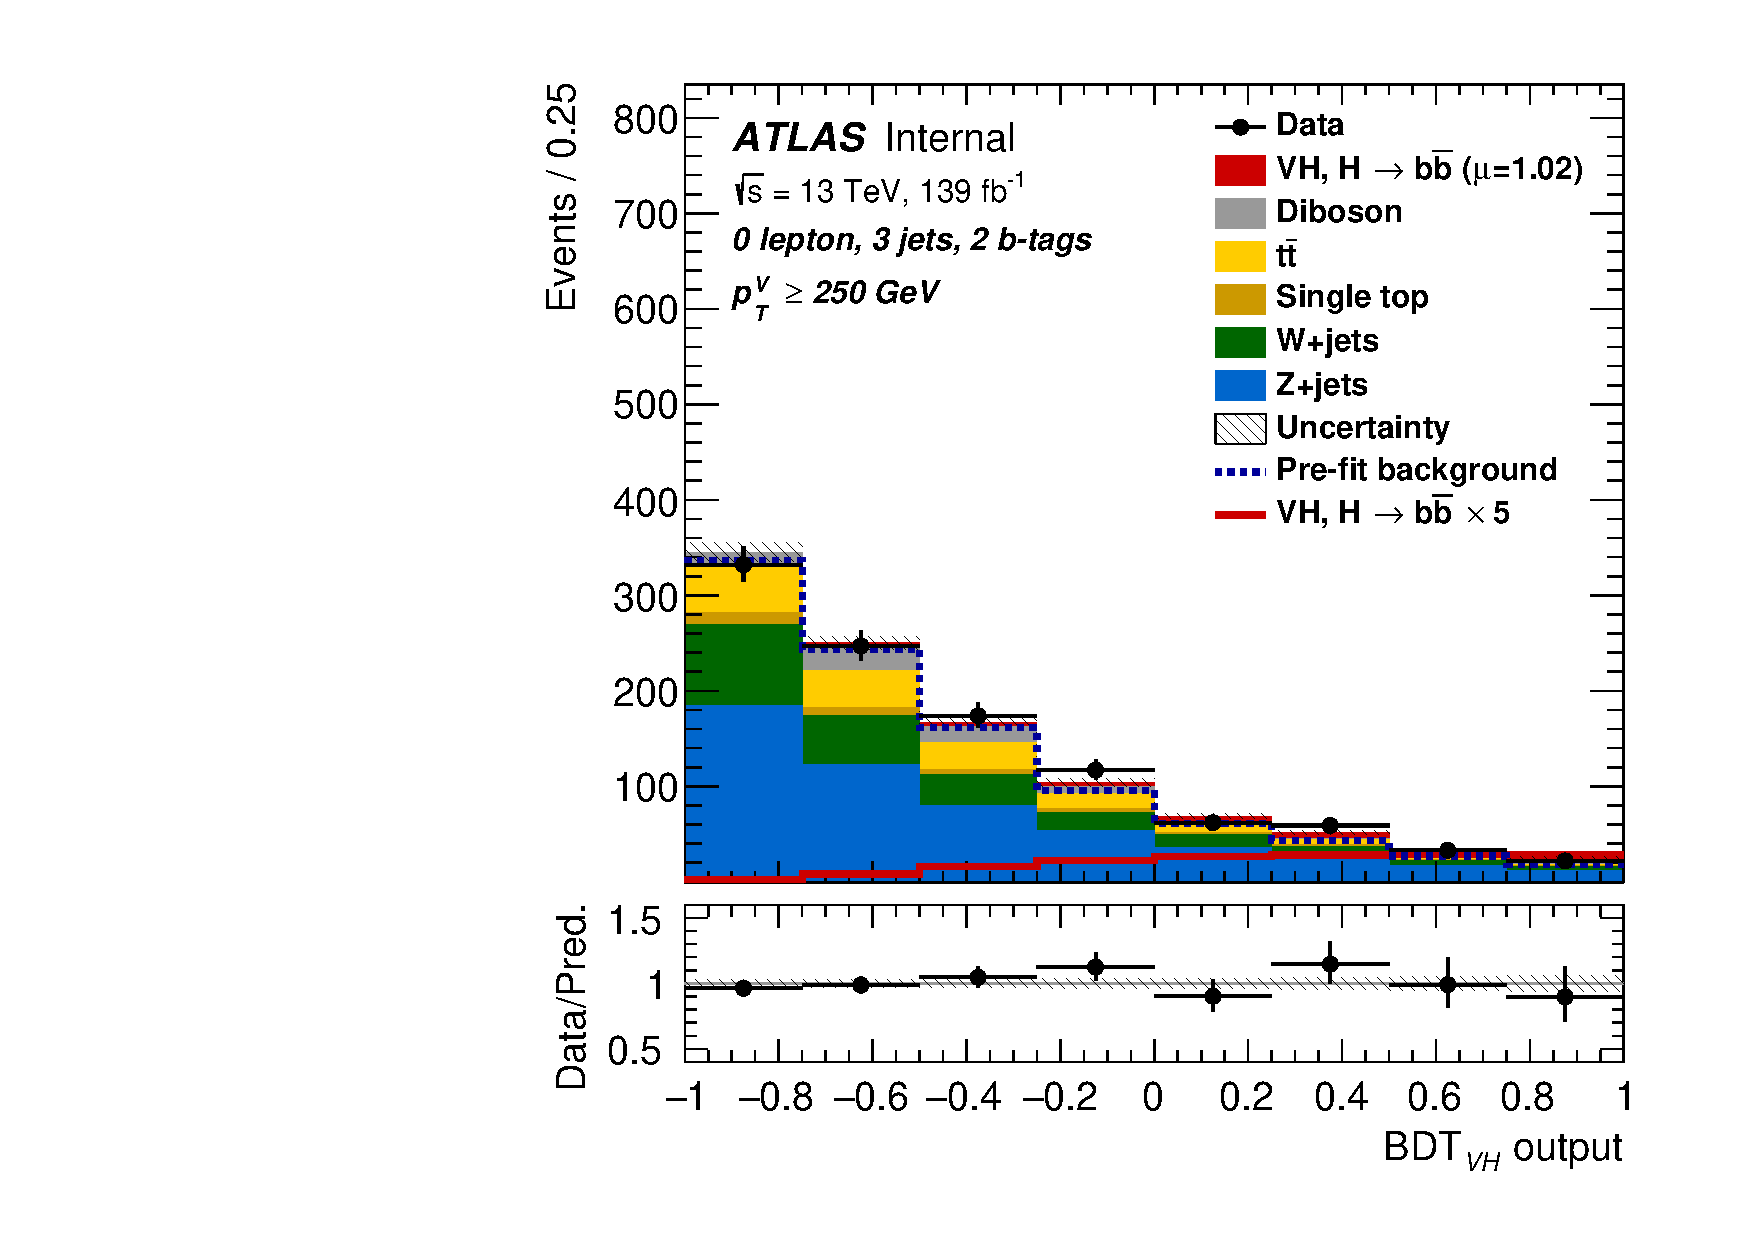
\includegraphics[width=.3\textwidth]{final_fit_mva/postfit/Region_BMin250_Y6051_DSR_T2_L0_distmva_J3_GlobalFit_unconditionnal_mu1} \\

    % bottom row
    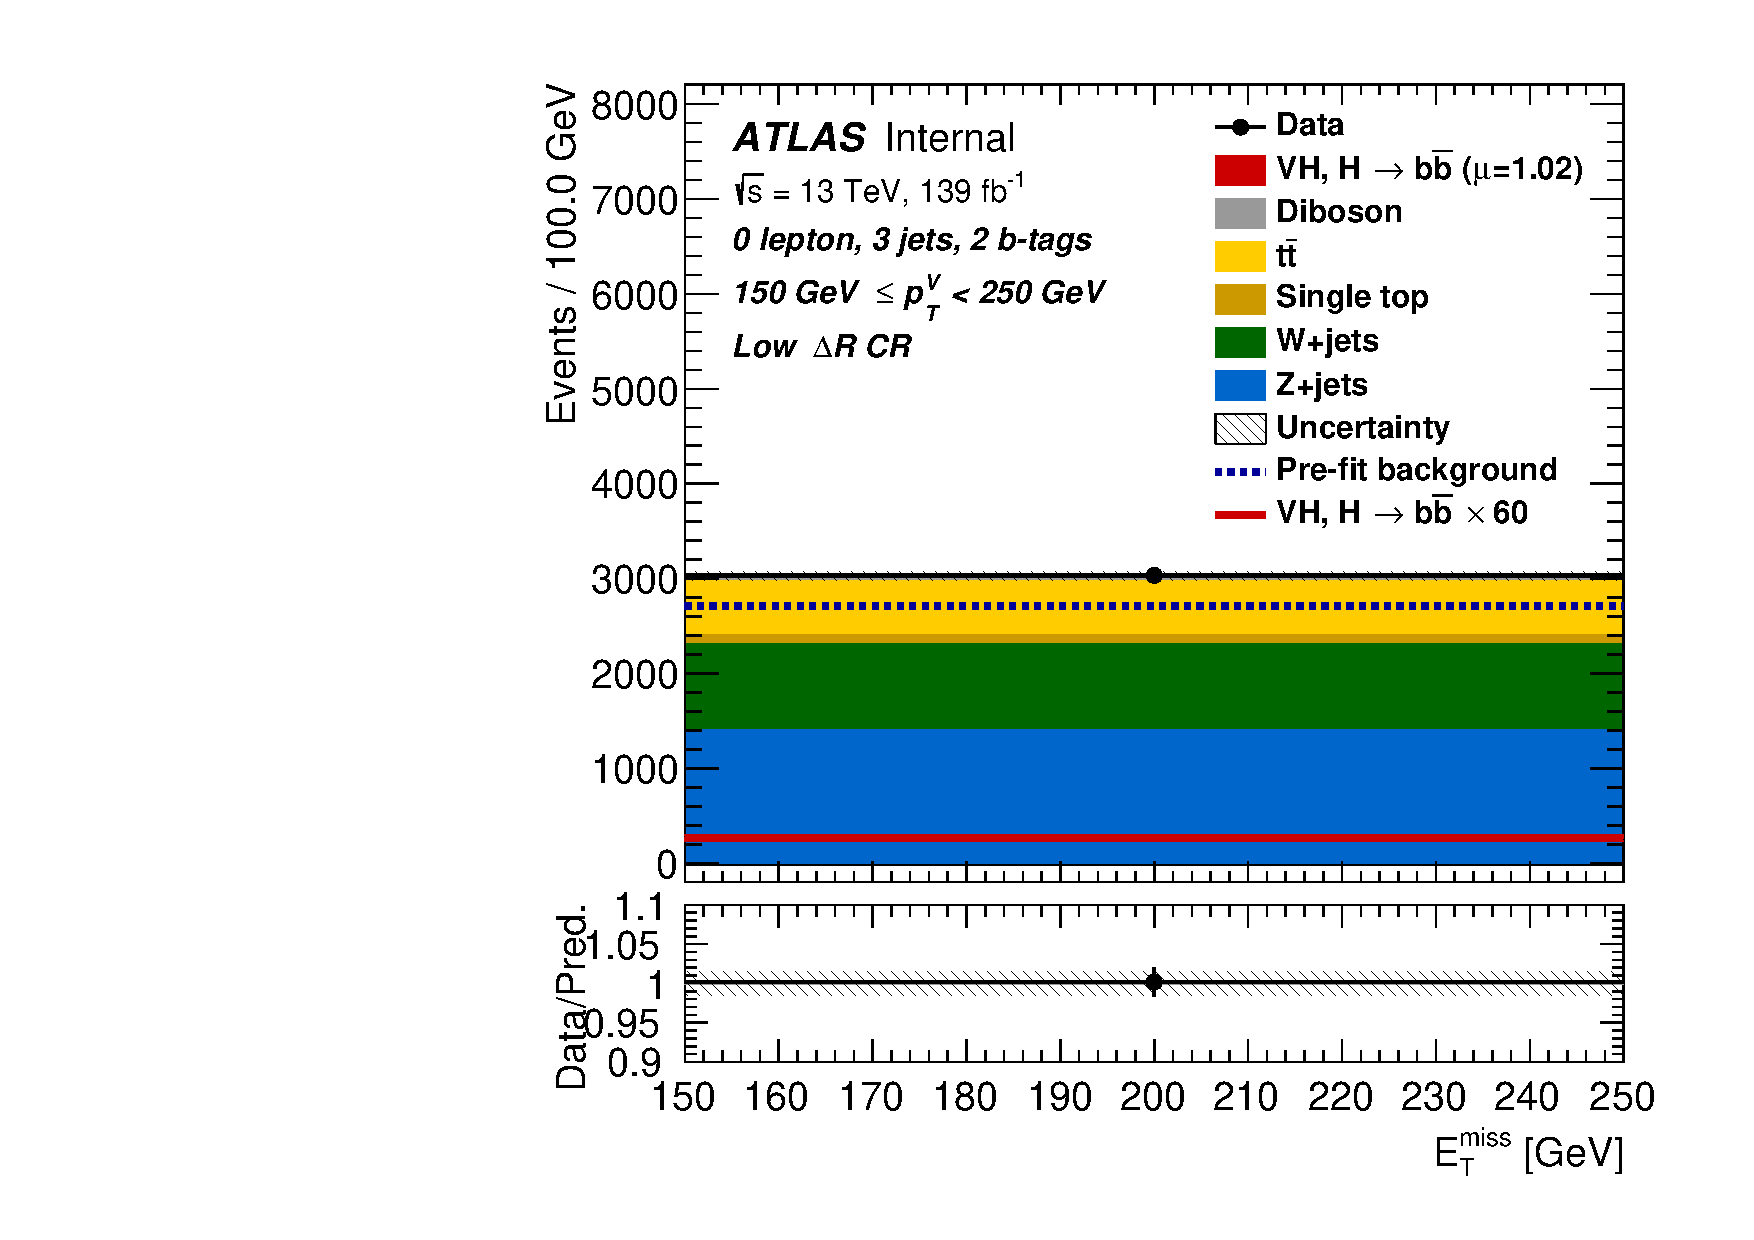
\includegraphics[width=.3\textwidth]{final_fit_mva/postfit/Region_BMax250_BMin150_Y6051_DCRLow_T2_L0_distMET_J3_GlobalFit_unconditionnal_mu1}%
    & 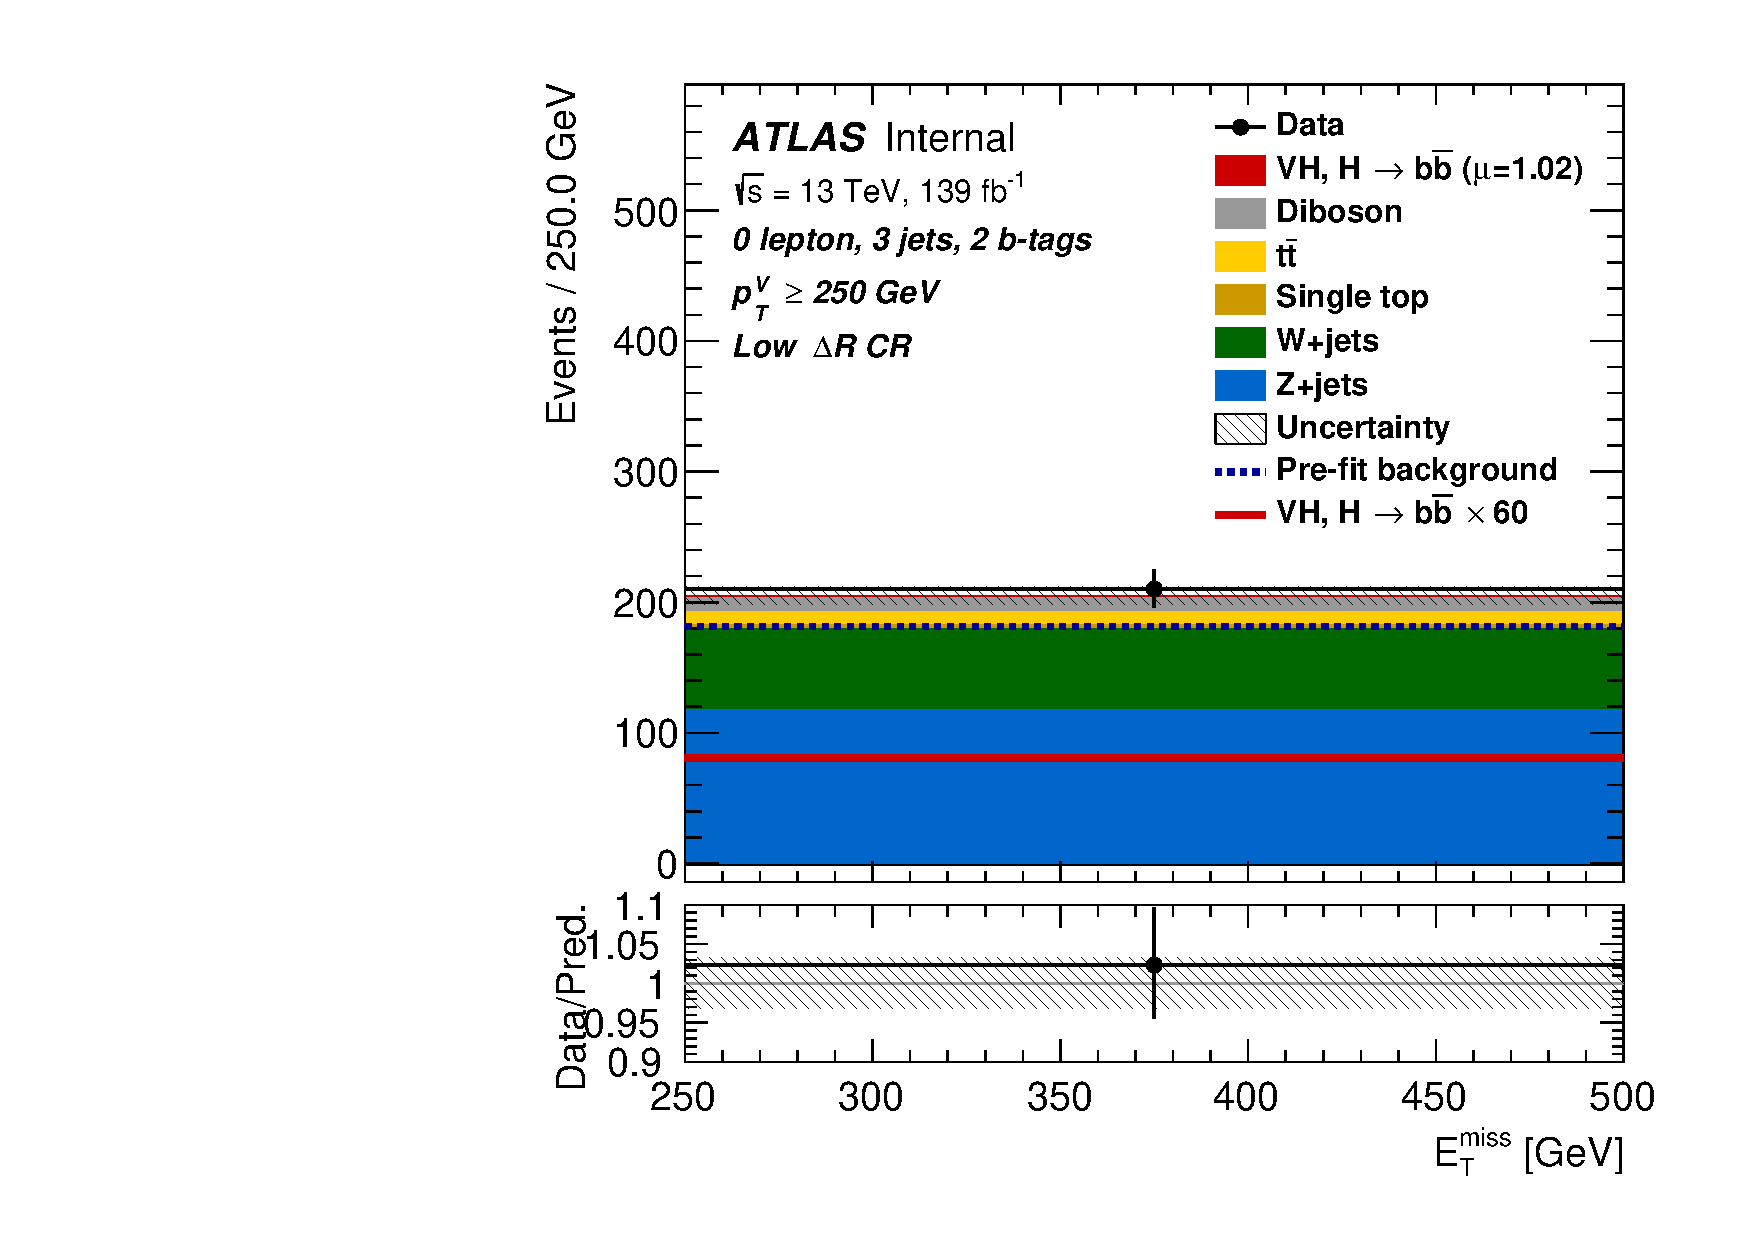
\includegraphics[width=.3\textwidth]{final_fit_mva/postfit/Region_BMin250_Y6051_DCRLow_T2_L0_distMET_J3_GlobalFit_unconditionnal_mu1} \\
  \end{tabular}
  \caption{Post-fit distributions in the 0 lepton 3 jet channel.}
\end{figure}
\begin{figure}
  \centering
  \begin{tabular}{cc}
    % top row
    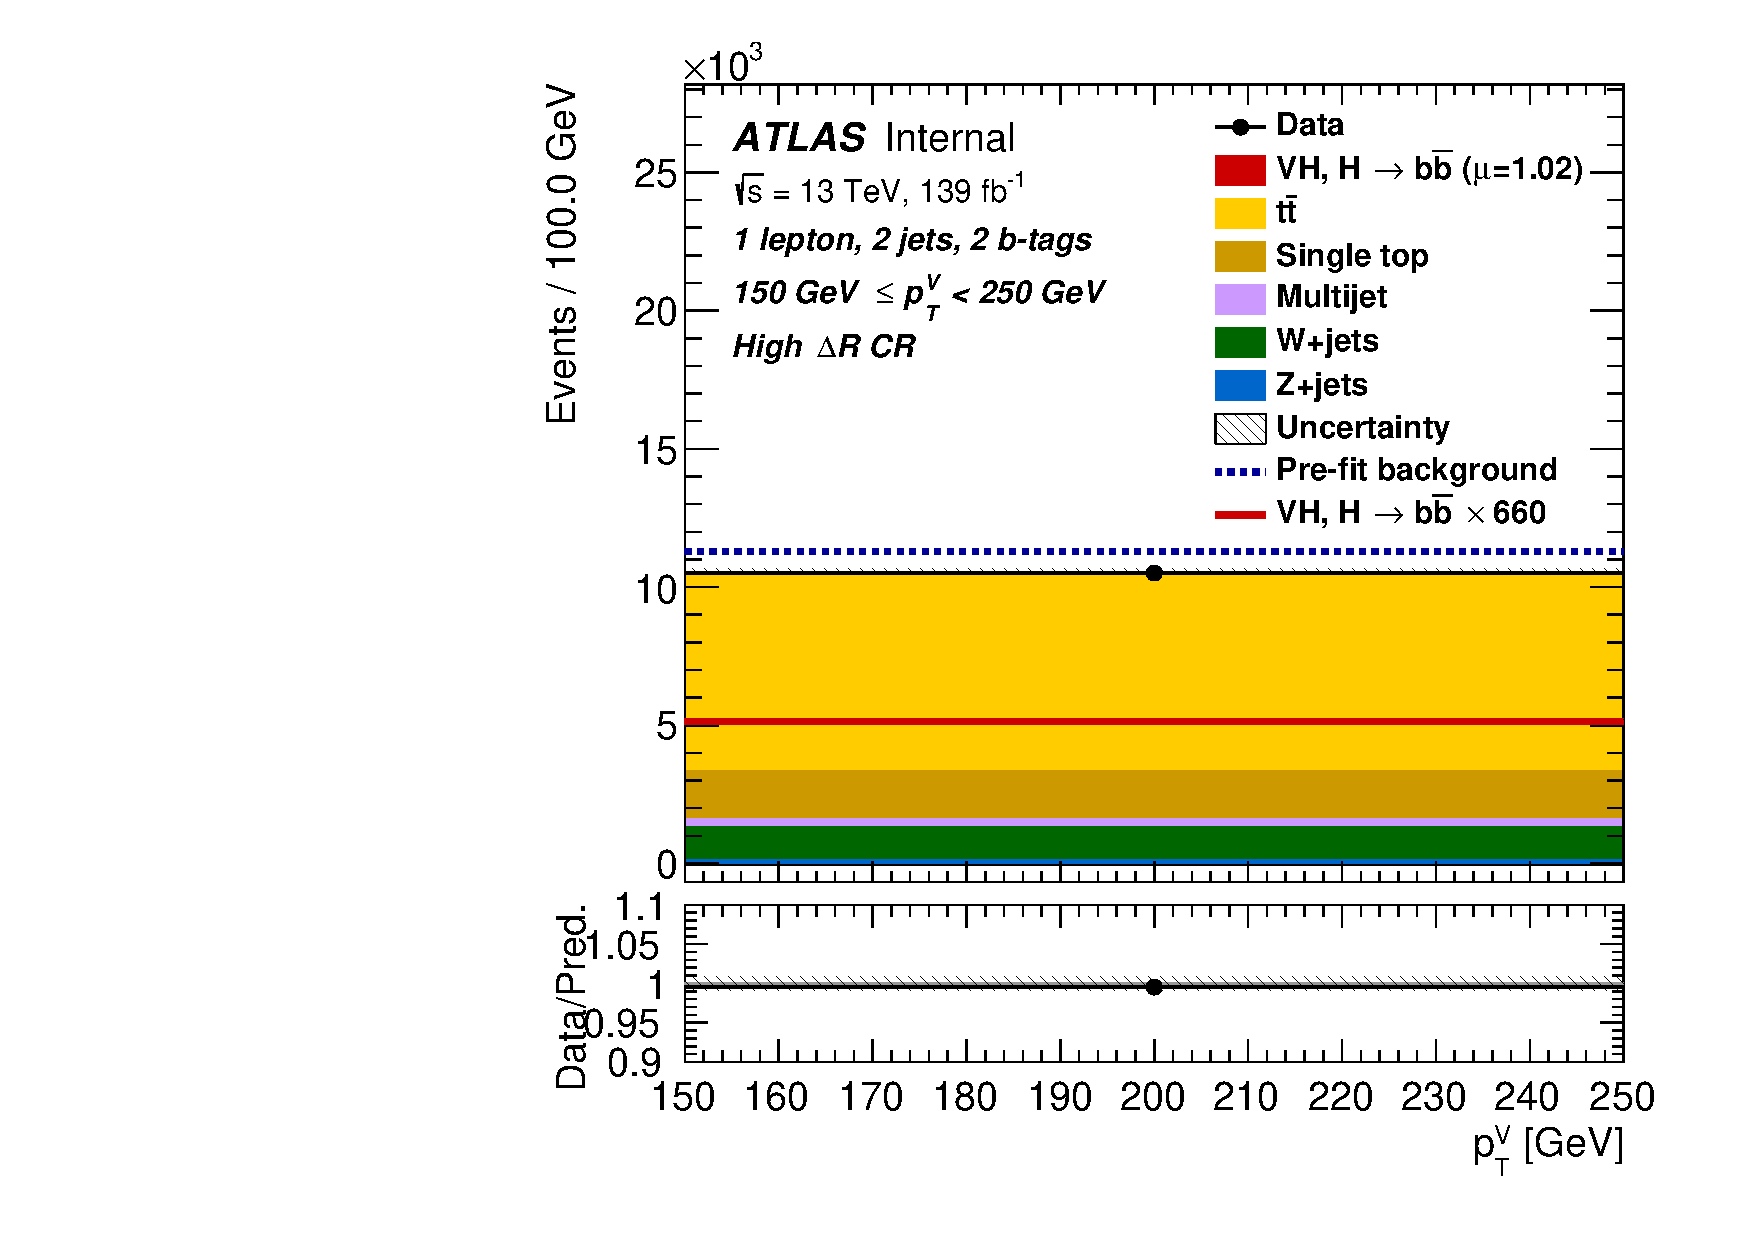
\includegraphics[width=.49\textwidth]{final_fit_mva/postfit/Region_BMax250_BMin150_Y6051_DCRHigh_T2_L1_distpTV_J2_GlobalFit_unconditionnal_mu1}%
    & 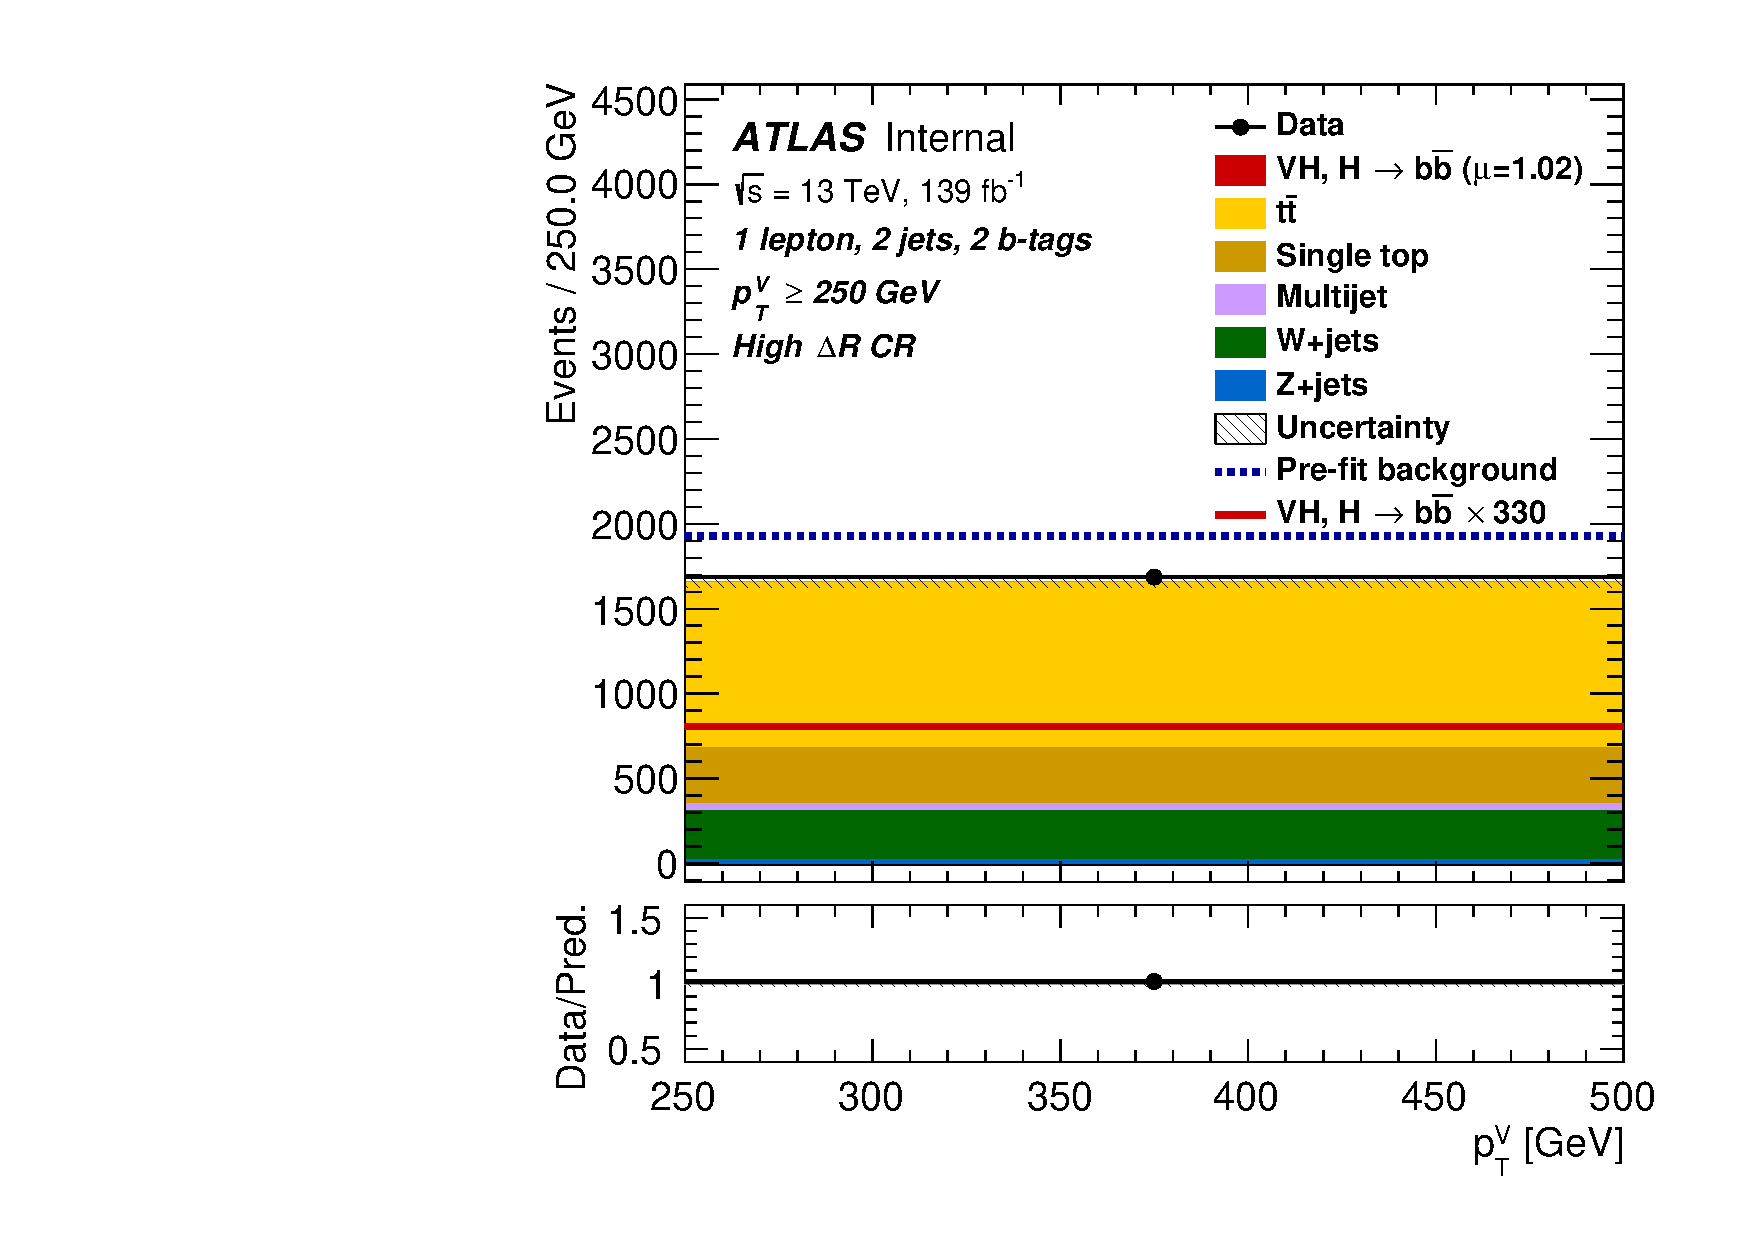
\includegraphics[width=.49\textwidth]{final_fit_mva/postfit/Region_BMin250_Y6051_DCRHigh_T2_L1_distpTV_J2_GlobalFit_unconditionnal_mu1} \\

    % middle row
    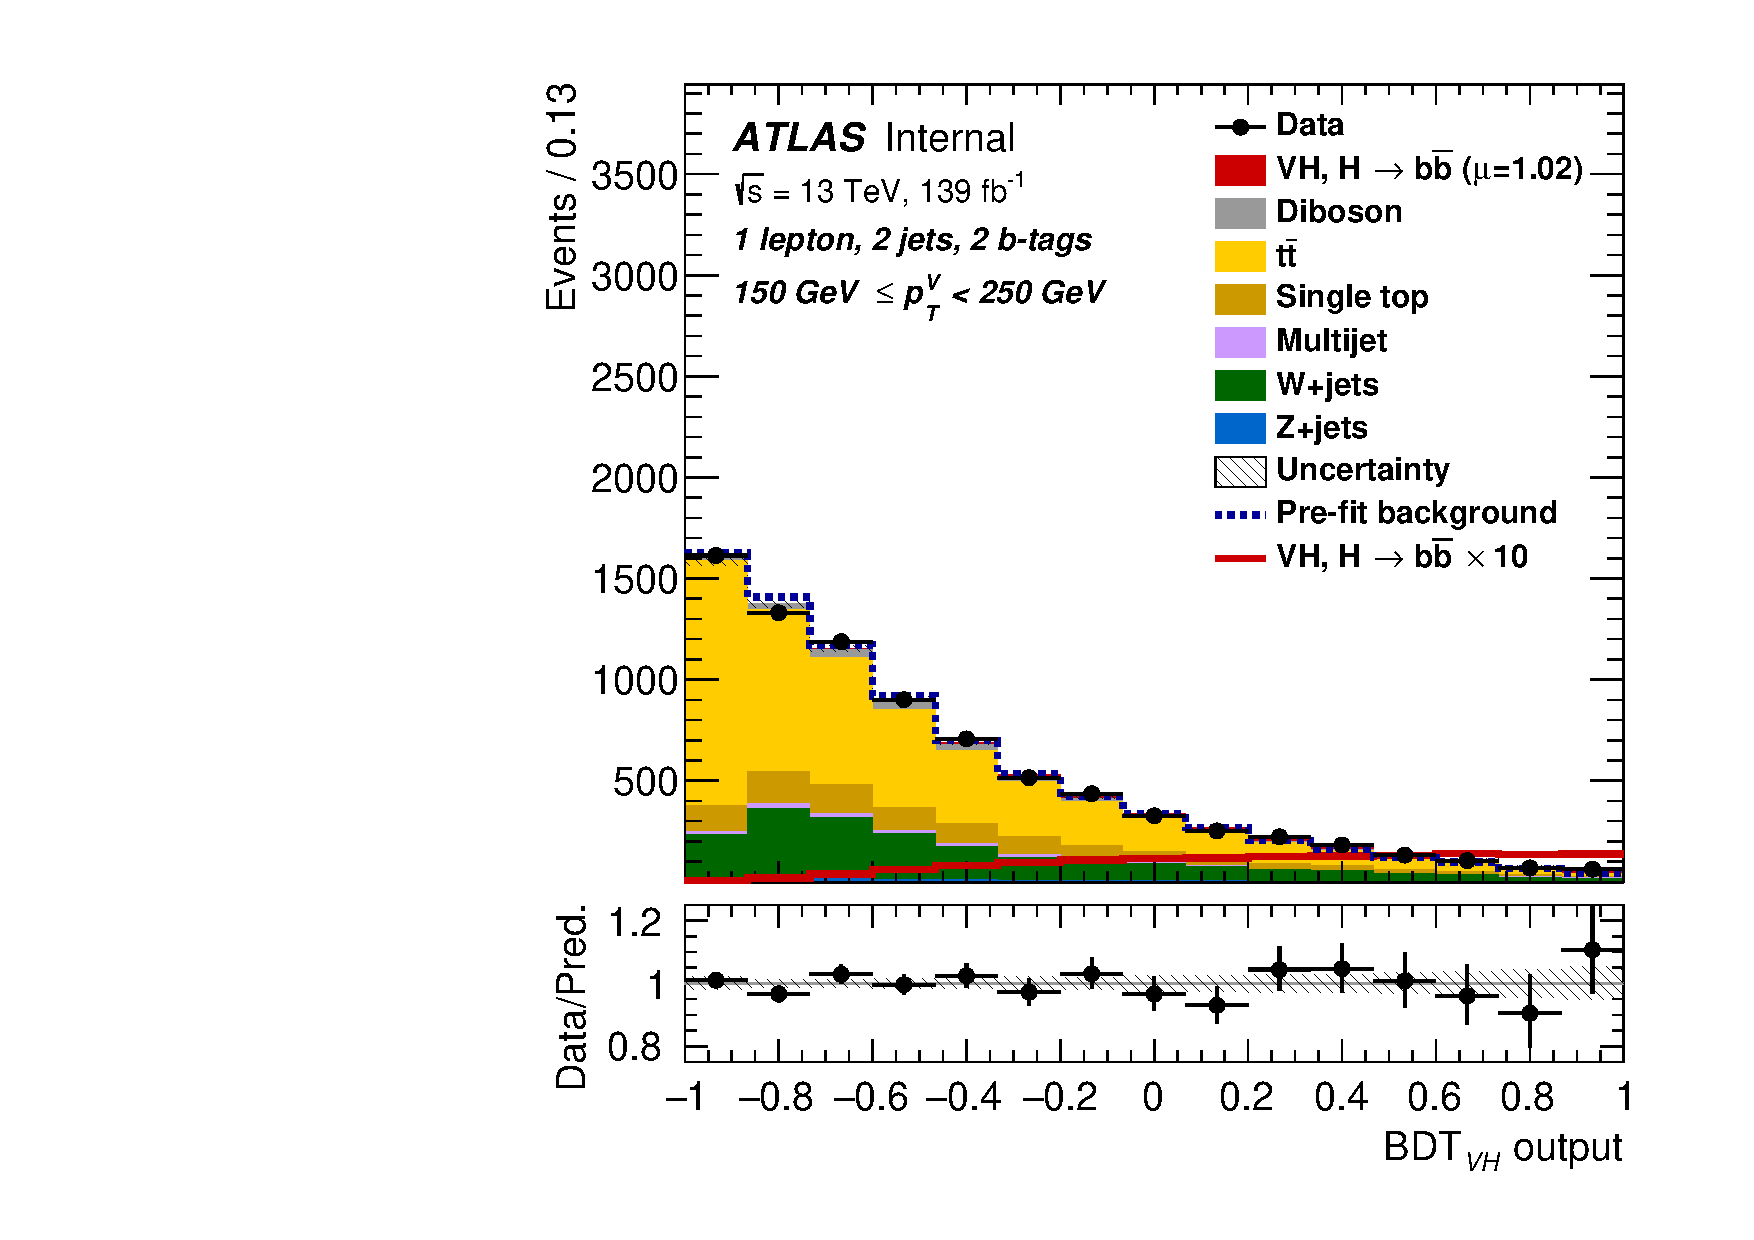
\includegraphics[width=.49\textwidth]{final_fit_mva/postfit/Region_BMax250_BMin150_Y6051_DSR_T2_L1_distmva_J2_GlobalFit_unconditionnal_mu1}%
    & 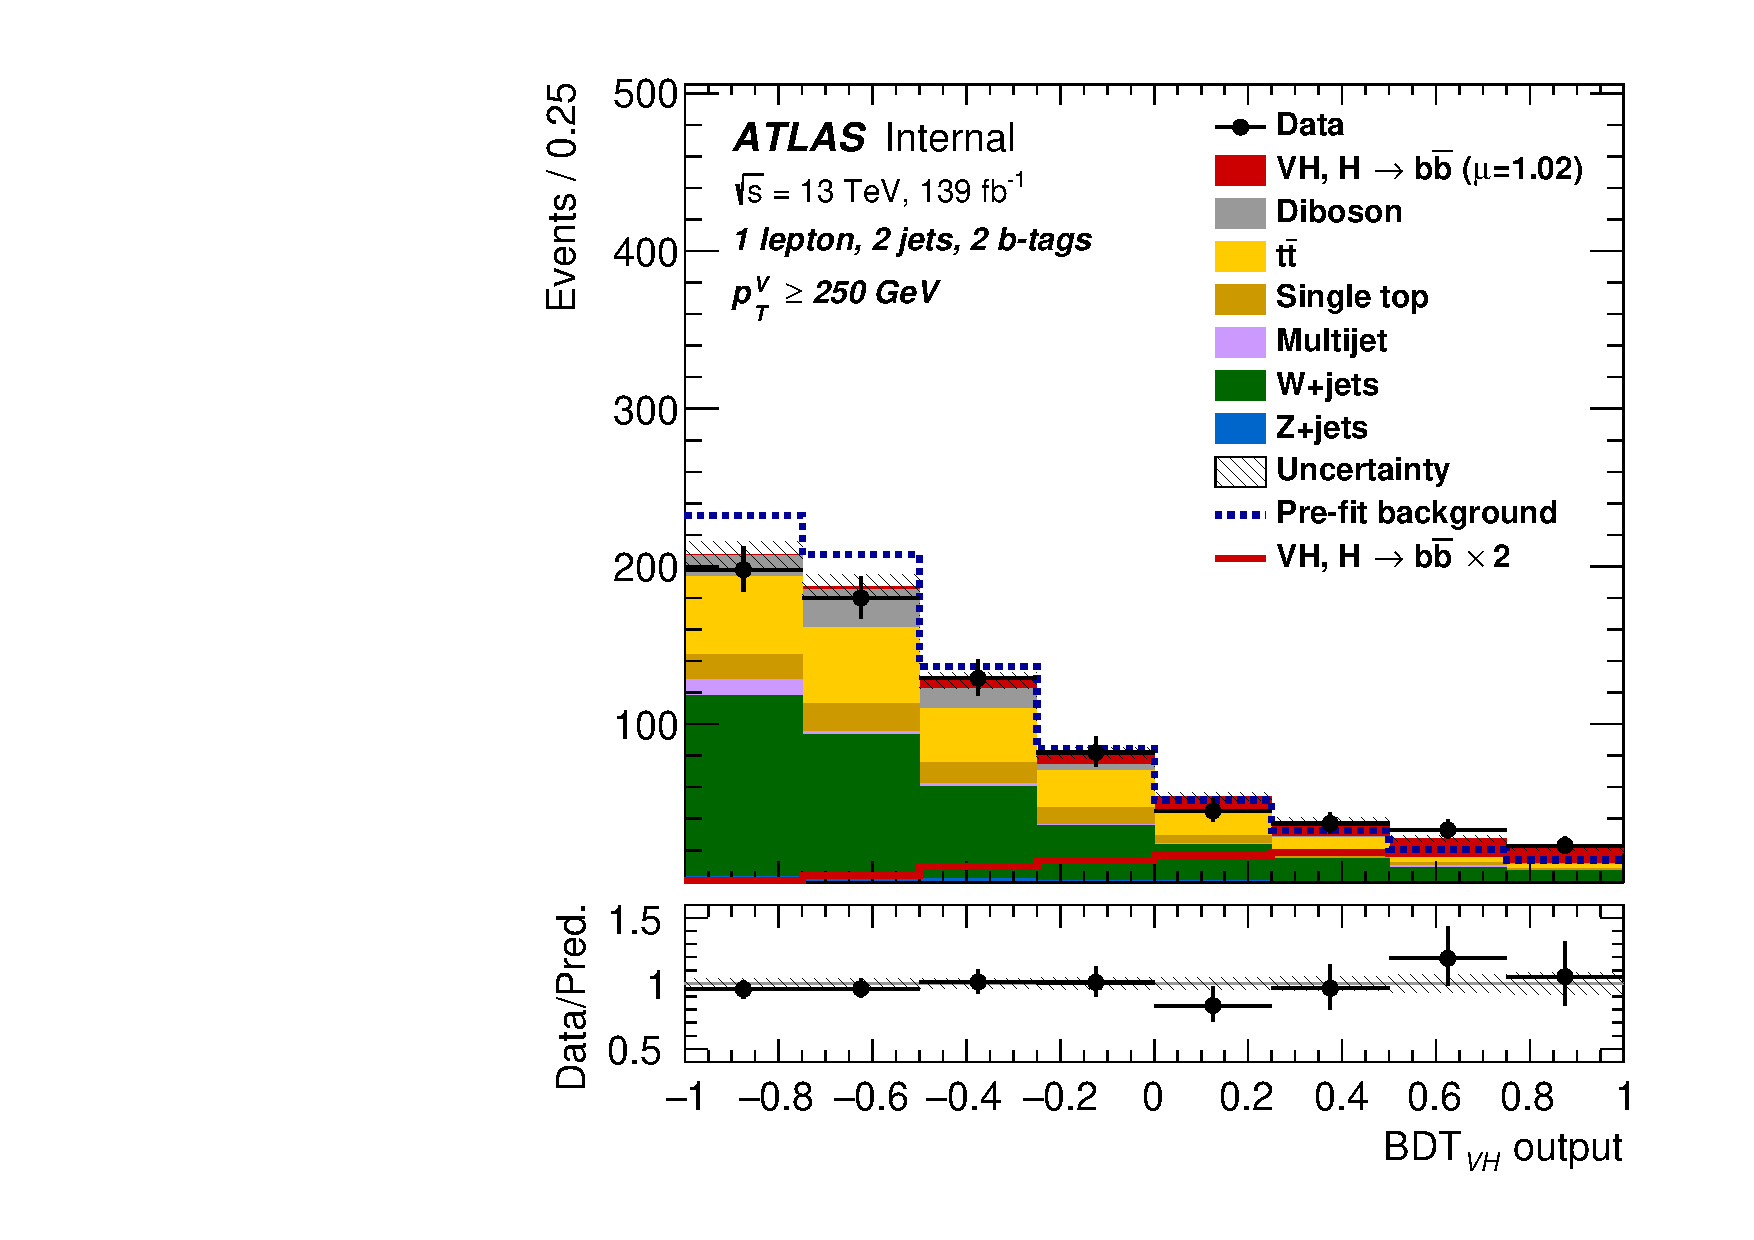
\includegraphics[width=.49\textwidth]{final_fit_mva/postfit/Region_BMin250_Y6051_DSR_T2_L1_distmva_J2_GlobalFit_unconditionnal_mu1} \\

    % bottom row
    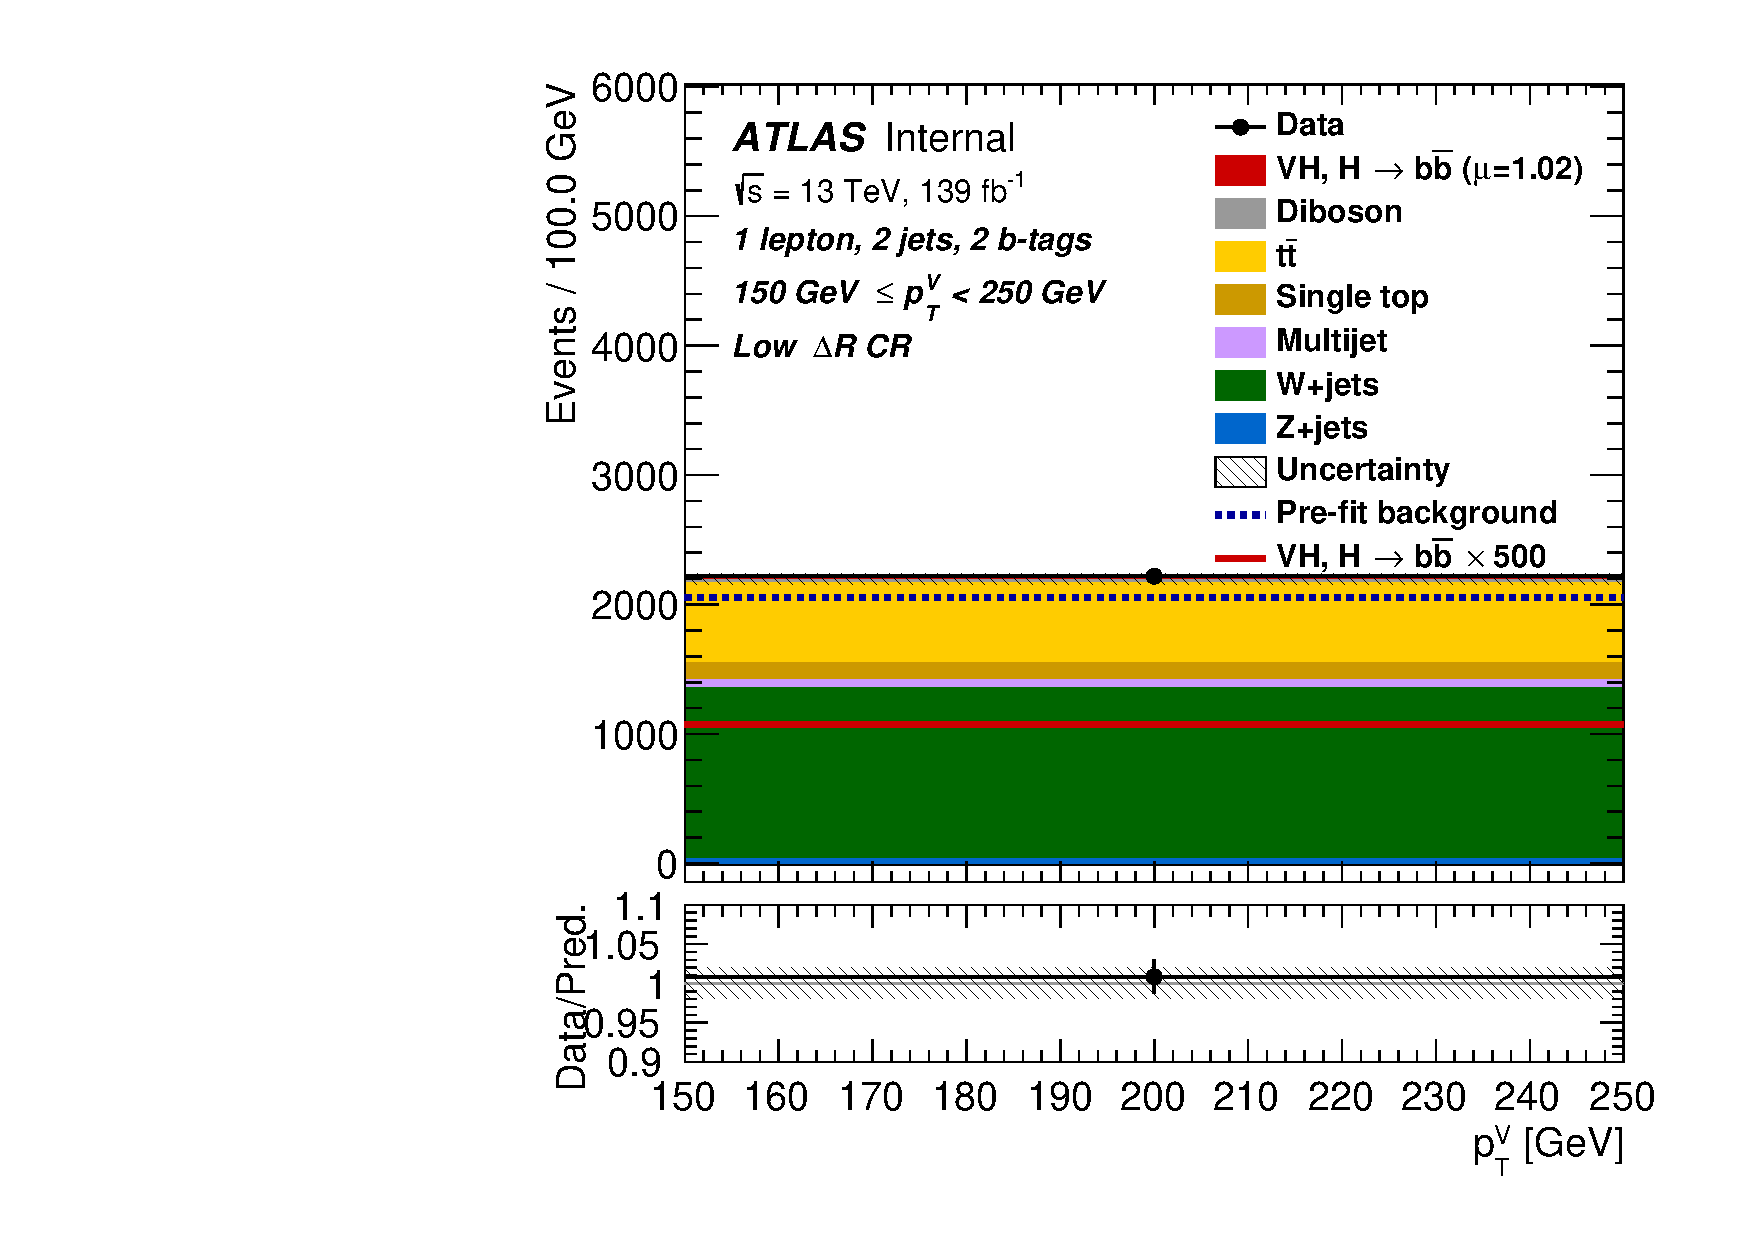
\includegraphics[width=.49\textwidth]{final_fit_mva/postfit/Region_BMax250_BMin150_Y6051_DCRLow_T2_L1_distpTV_J2_GlobalFit_unconditionnal_mu1}%
    & 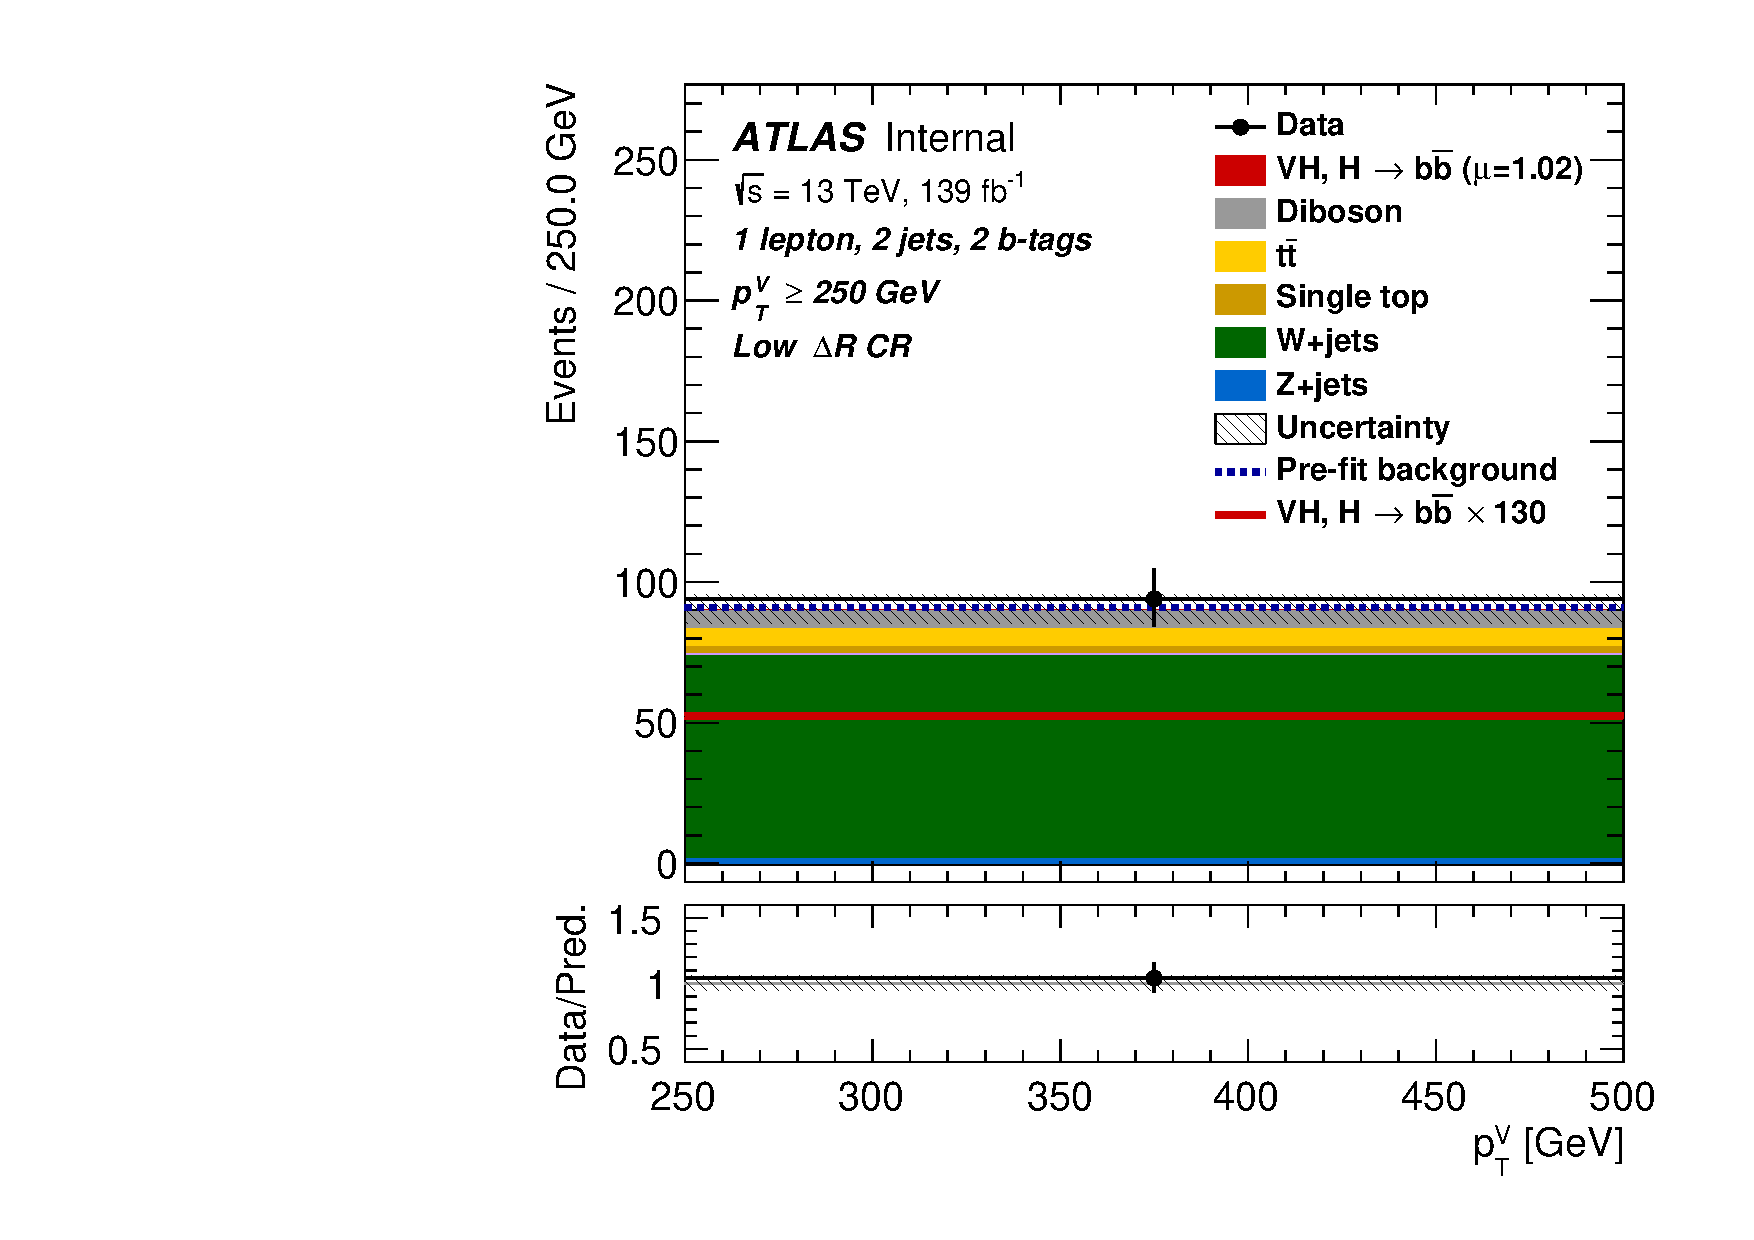
\includegraphics[width=.49\textwidth]{final_fit_mva/postfit/Region_BMin250_Y6051_DCRLow_T2_L1_distpTV_J2_GlobalFit_unconditionnal_mu1} \\
  \end{tabular}
  \caption{Post-fit distributions in the 1--lepton 2--jet channel.}
\end{figure}
\begin{figure}
  \centering
  \begin{tabular}{cc}
    % top row
    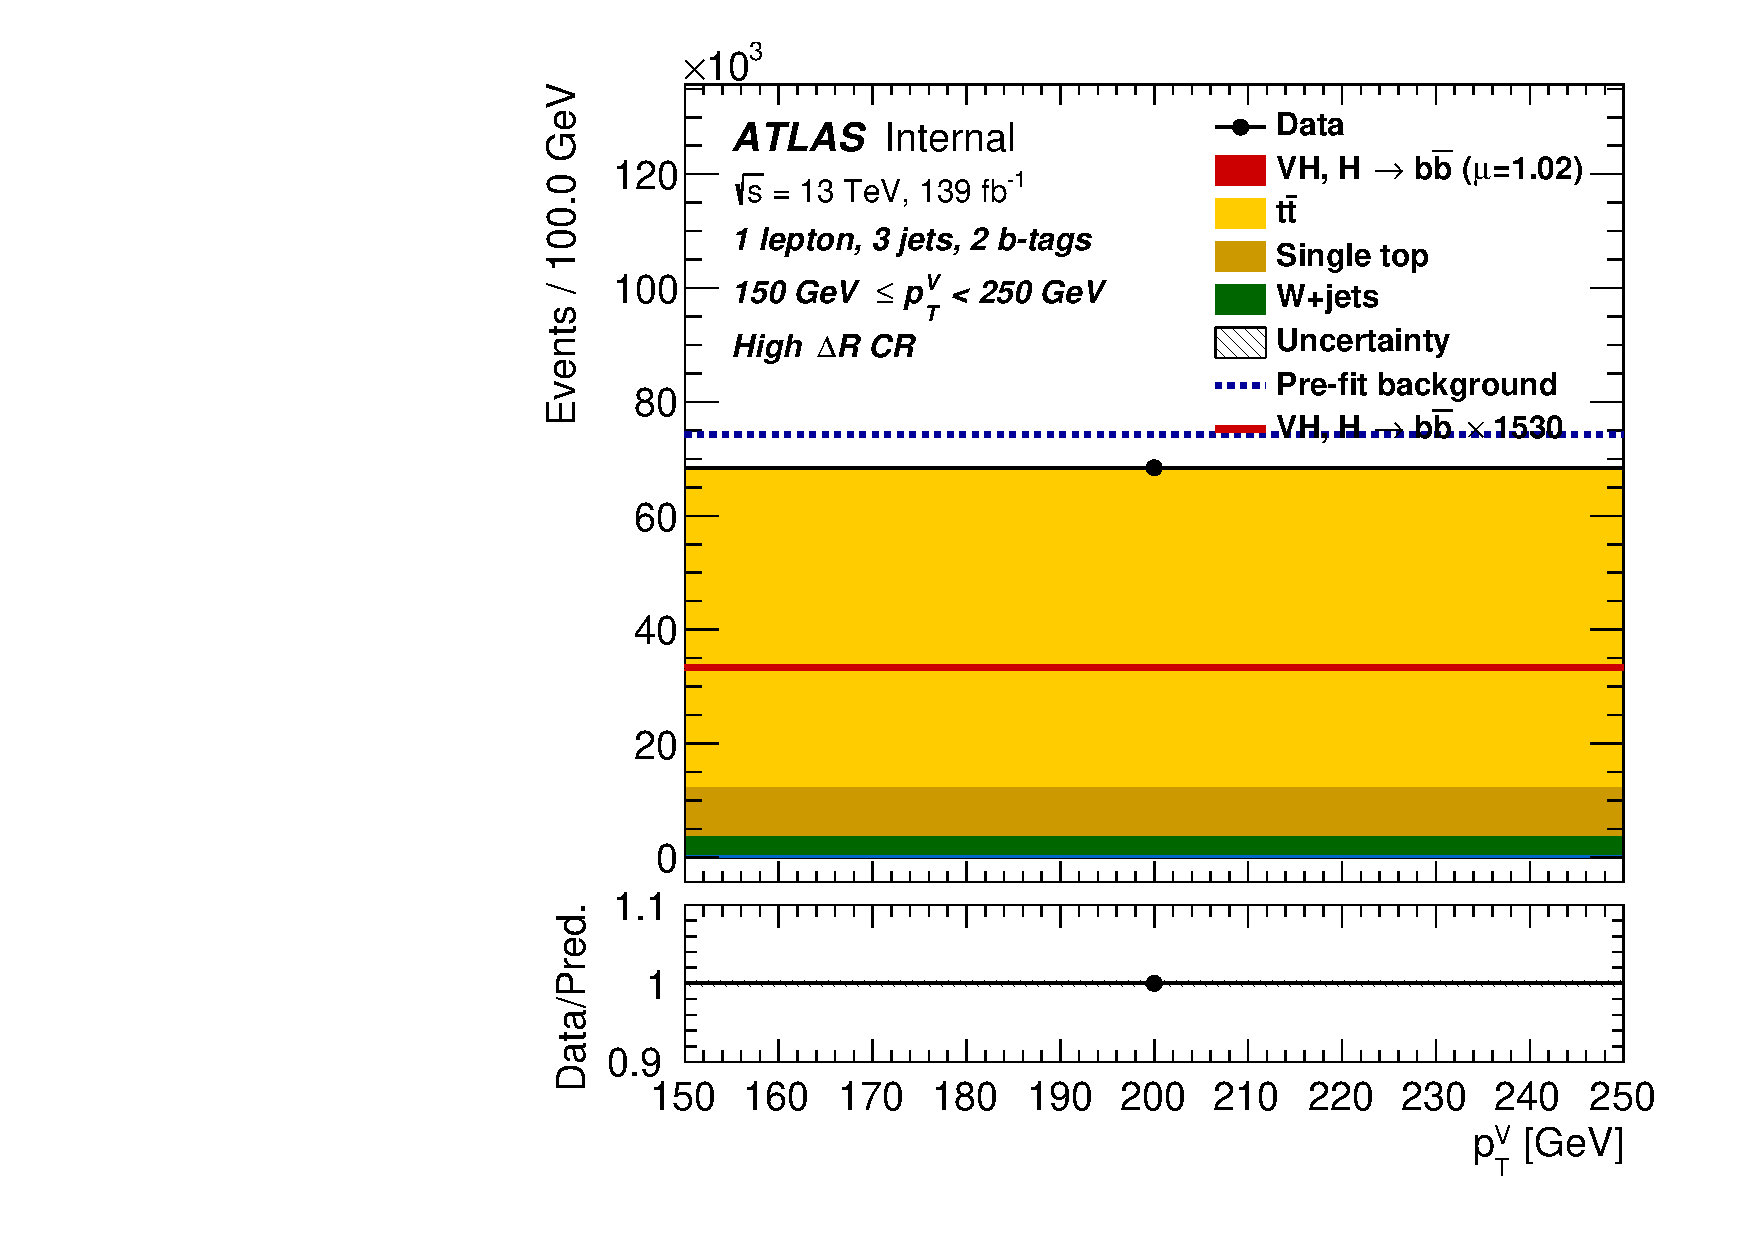
\includegraphics[width=.3\textwidth]{final_fit_mva/postfit/Region_BMax250_BMin150_Y6051_DCRHigh_T2_L1_distpTV_J3_GlobalFit_unconditionnal_mu1}%
    & 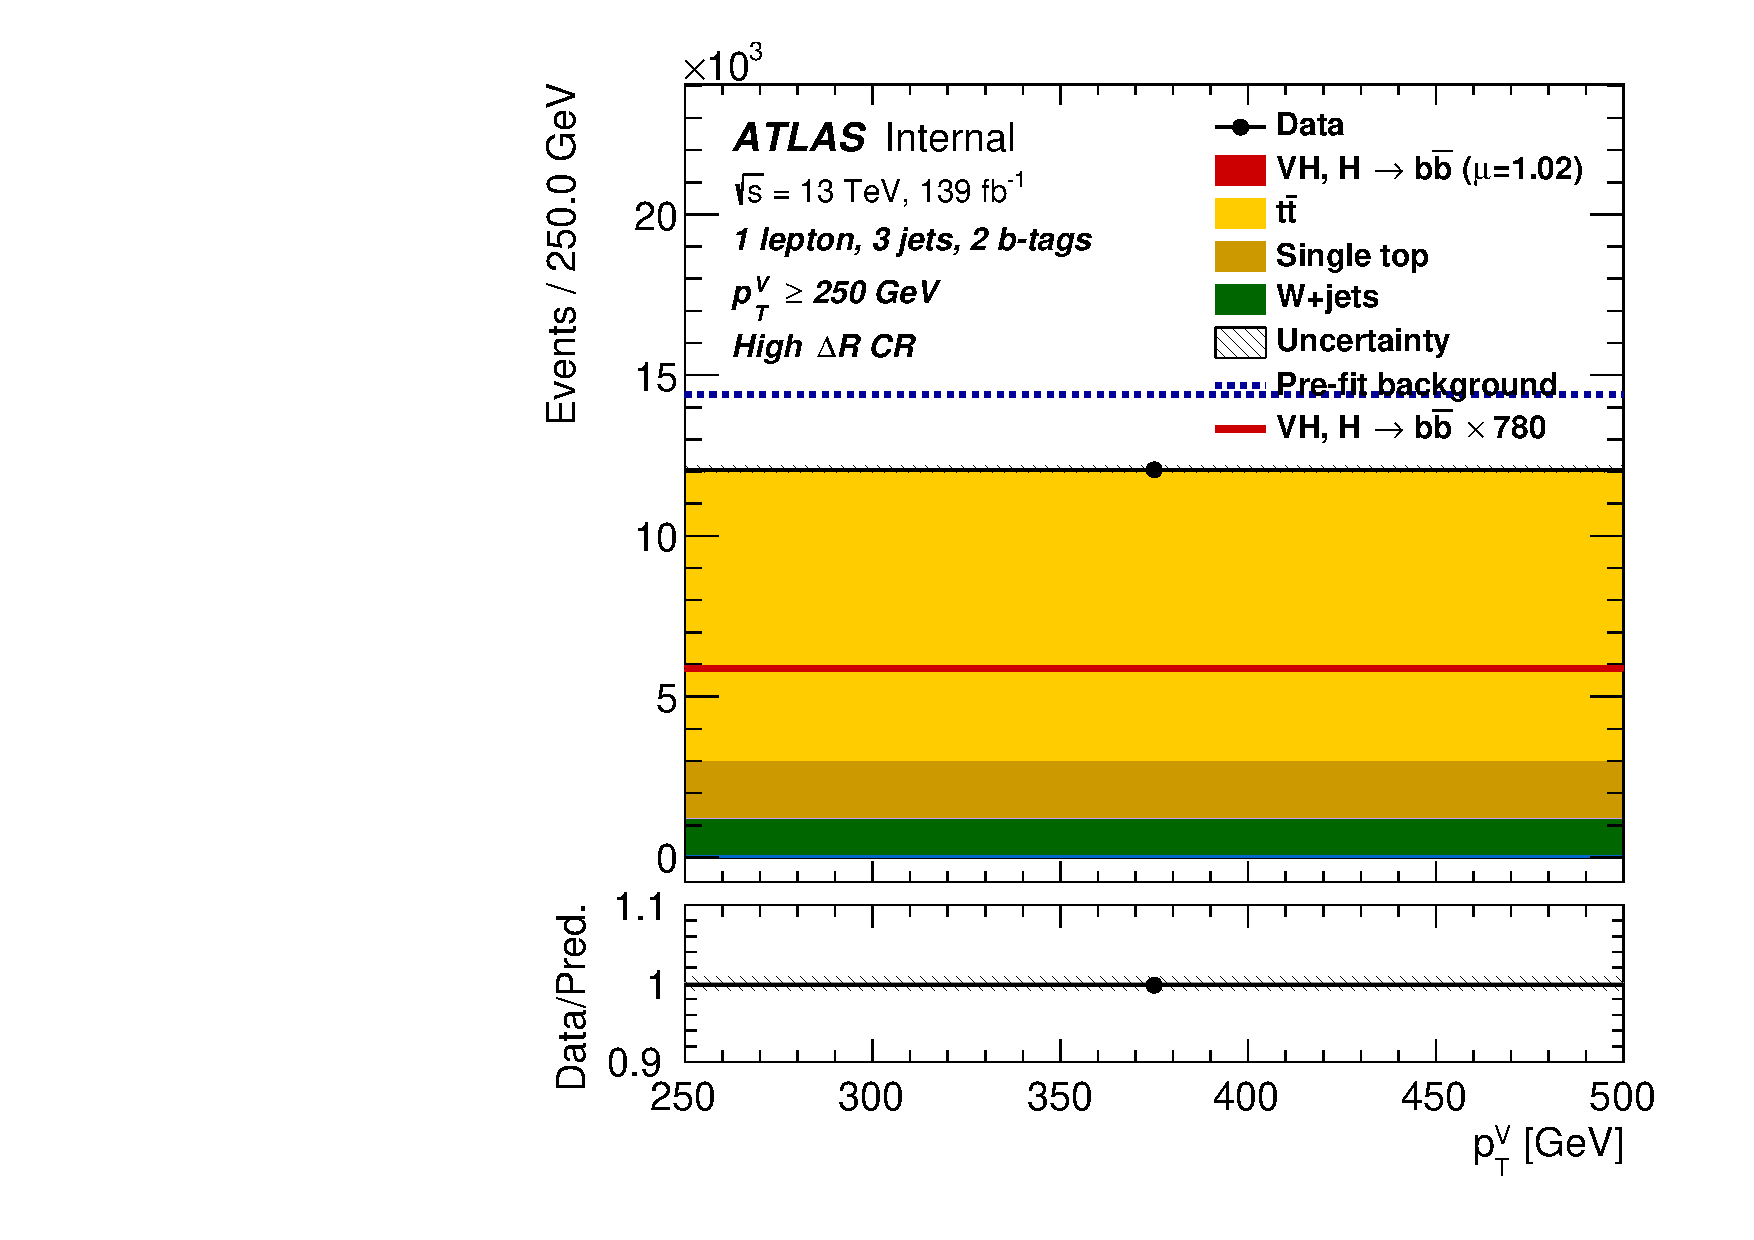
\includegraphics[width=.3\textwidth]{final_fit_mva/postfit/Region_BMin250_Y6051_DCRHigh_T2_L1_distpTV_J3_GlobalFit_unconditionnal_mu1} \\

    % middle row
    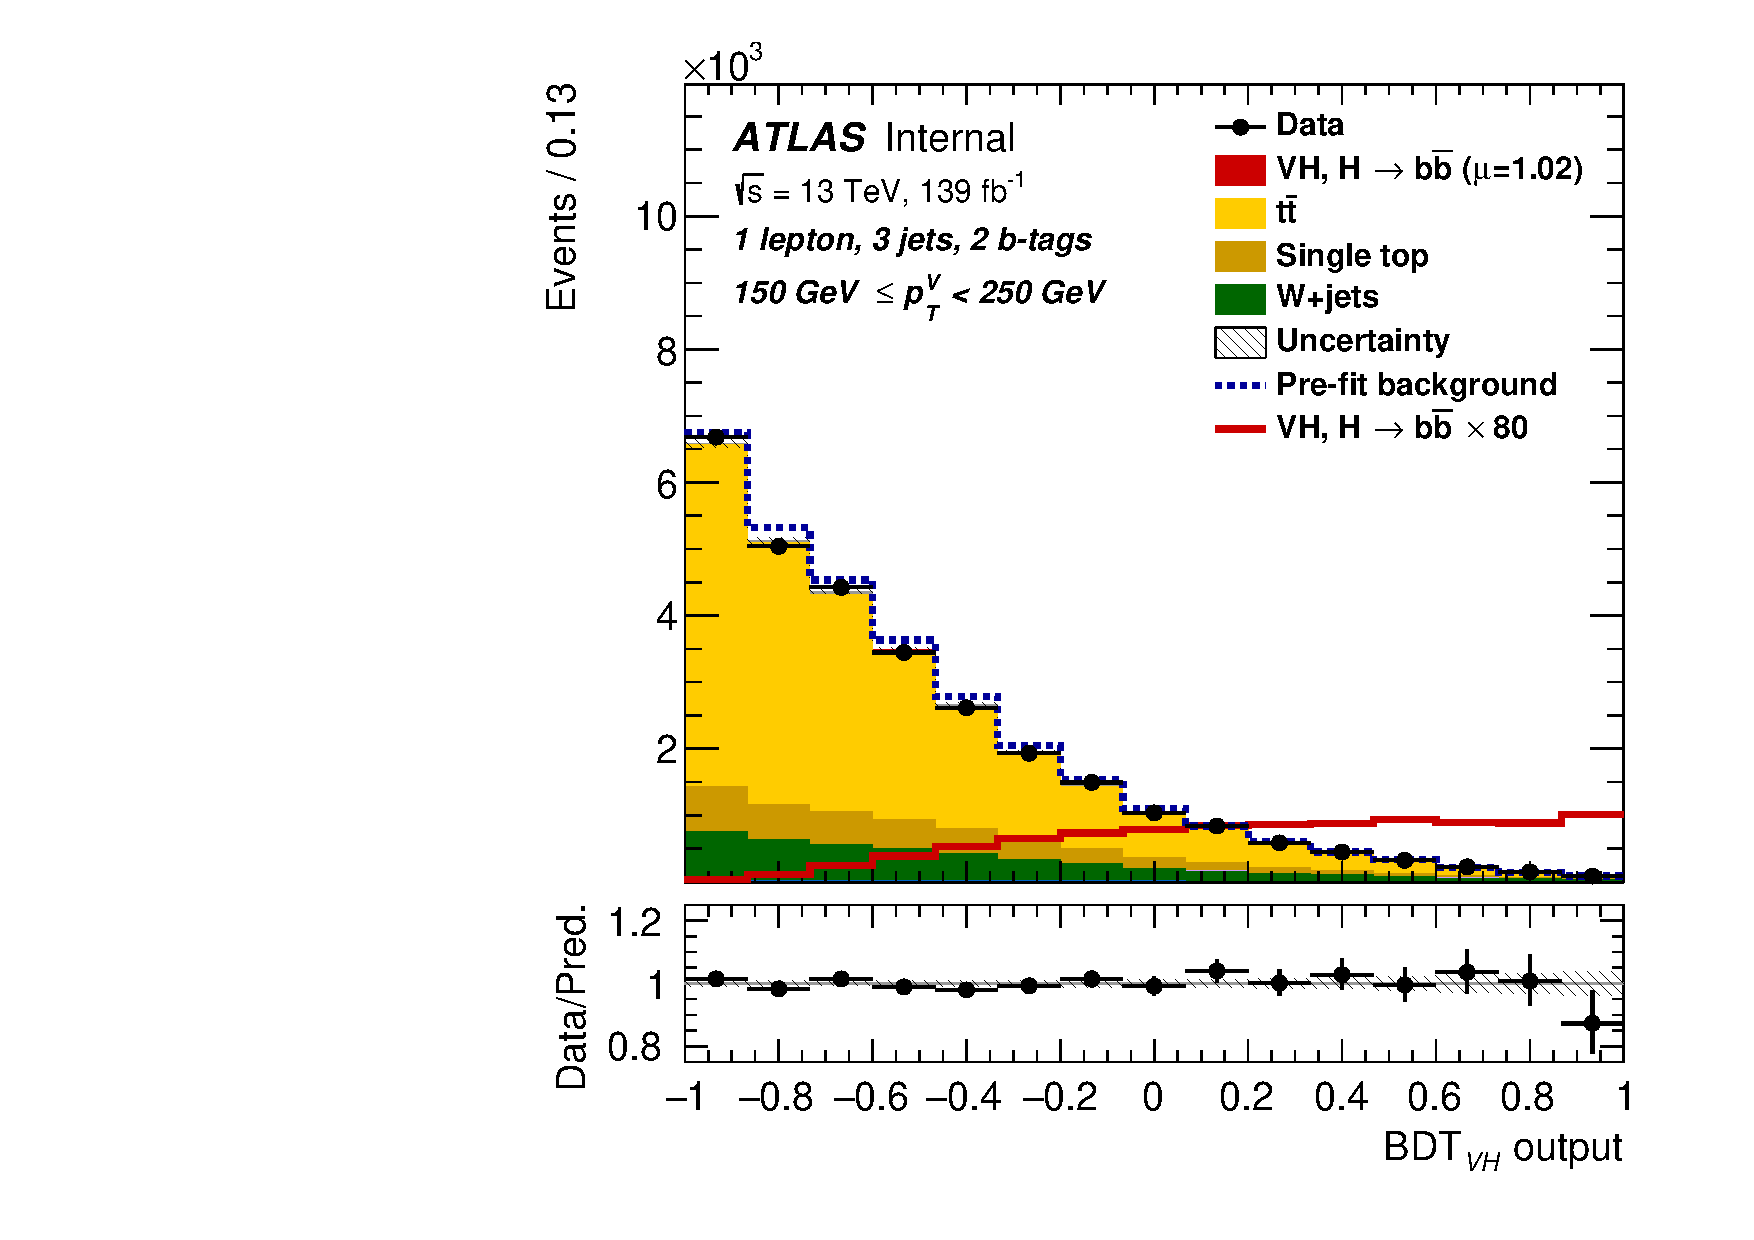
\includegraphics[width=.3\textwidth]{final_fit_mva/postfit/Region_BMax250_BMin150_Y6051_DSR_T2_L1_distmva_J3_GlobalFit_unconditionnal_mu1}%
    & 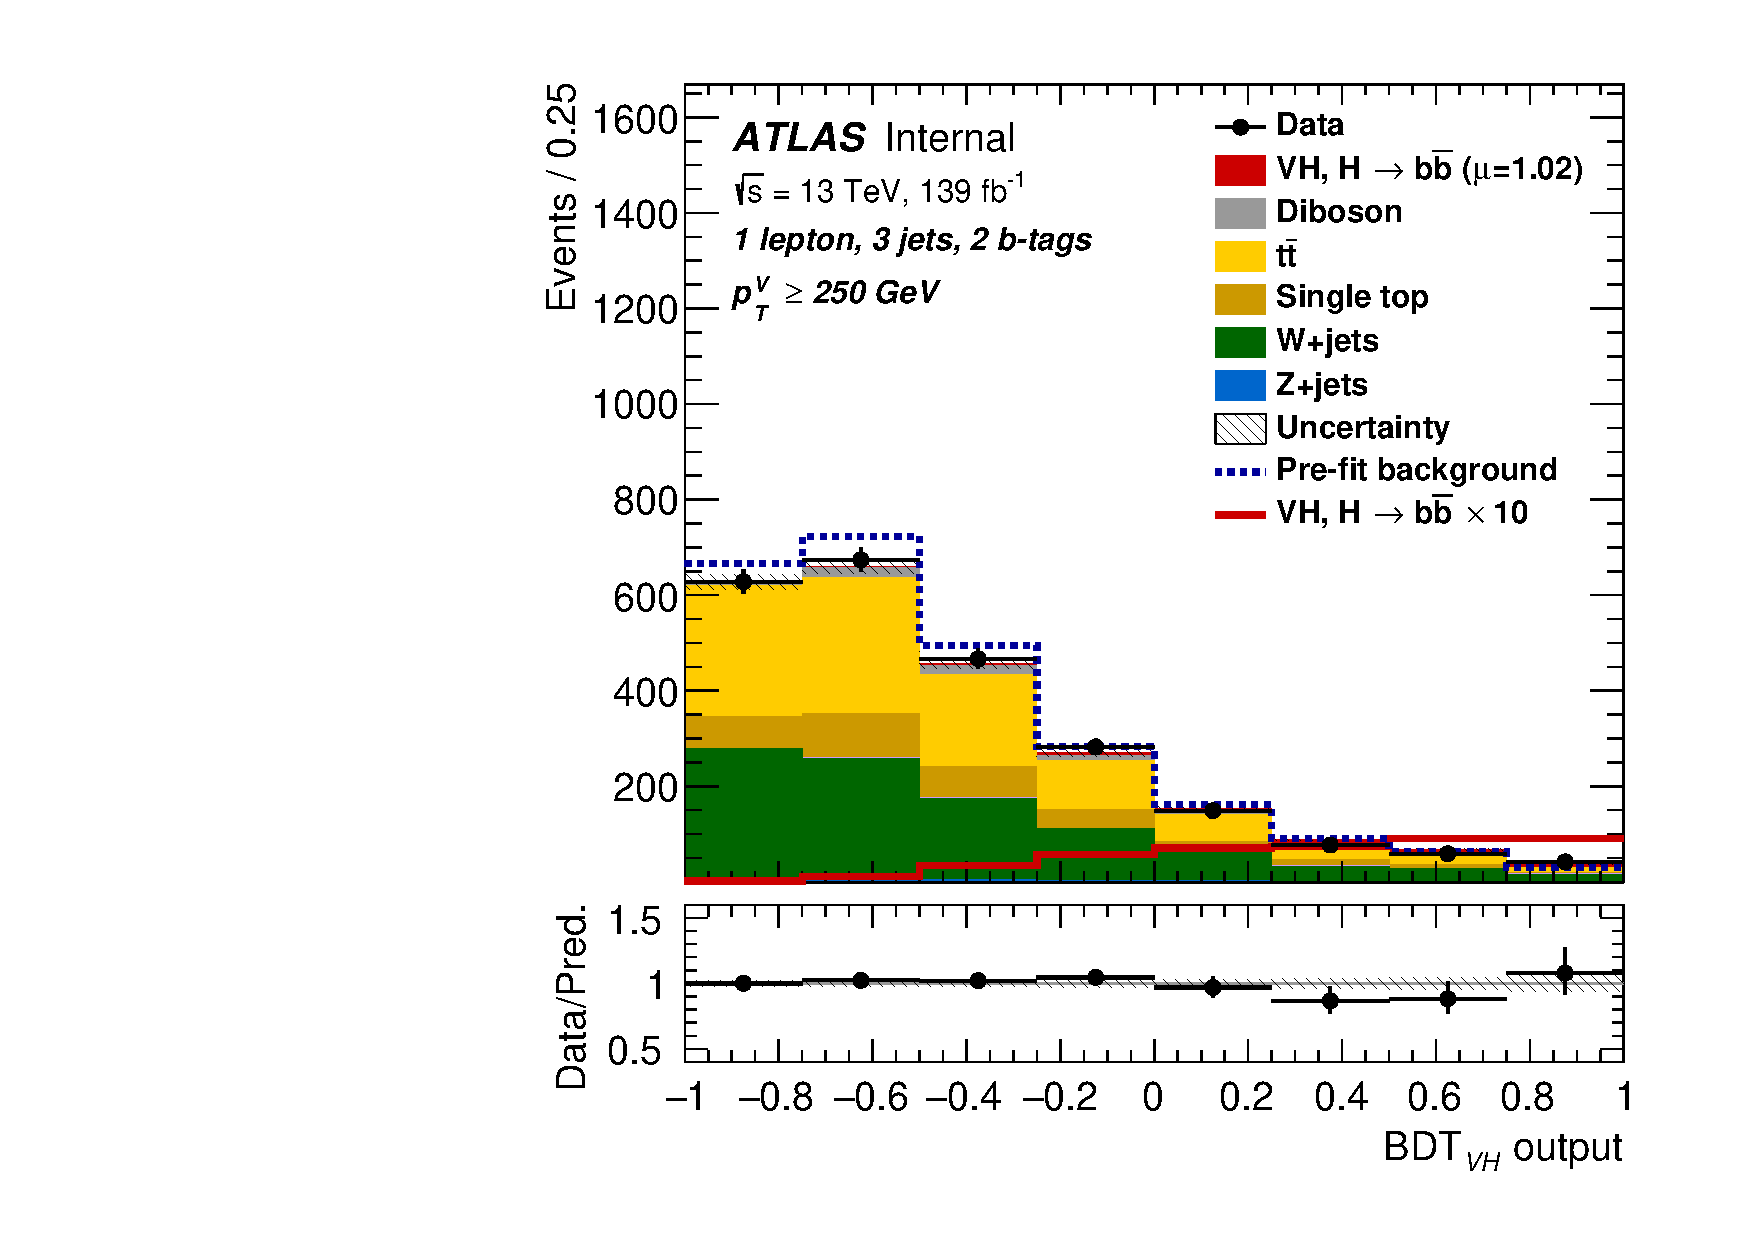
\includegraphics[width=.3\textwidth]{final_fit_mva/postfit/Region_BMin250_Y6051_DSR_T2_L1_distmva_J3_GlobalFit_unconditionnal_mu1} \\

    % bottom row
    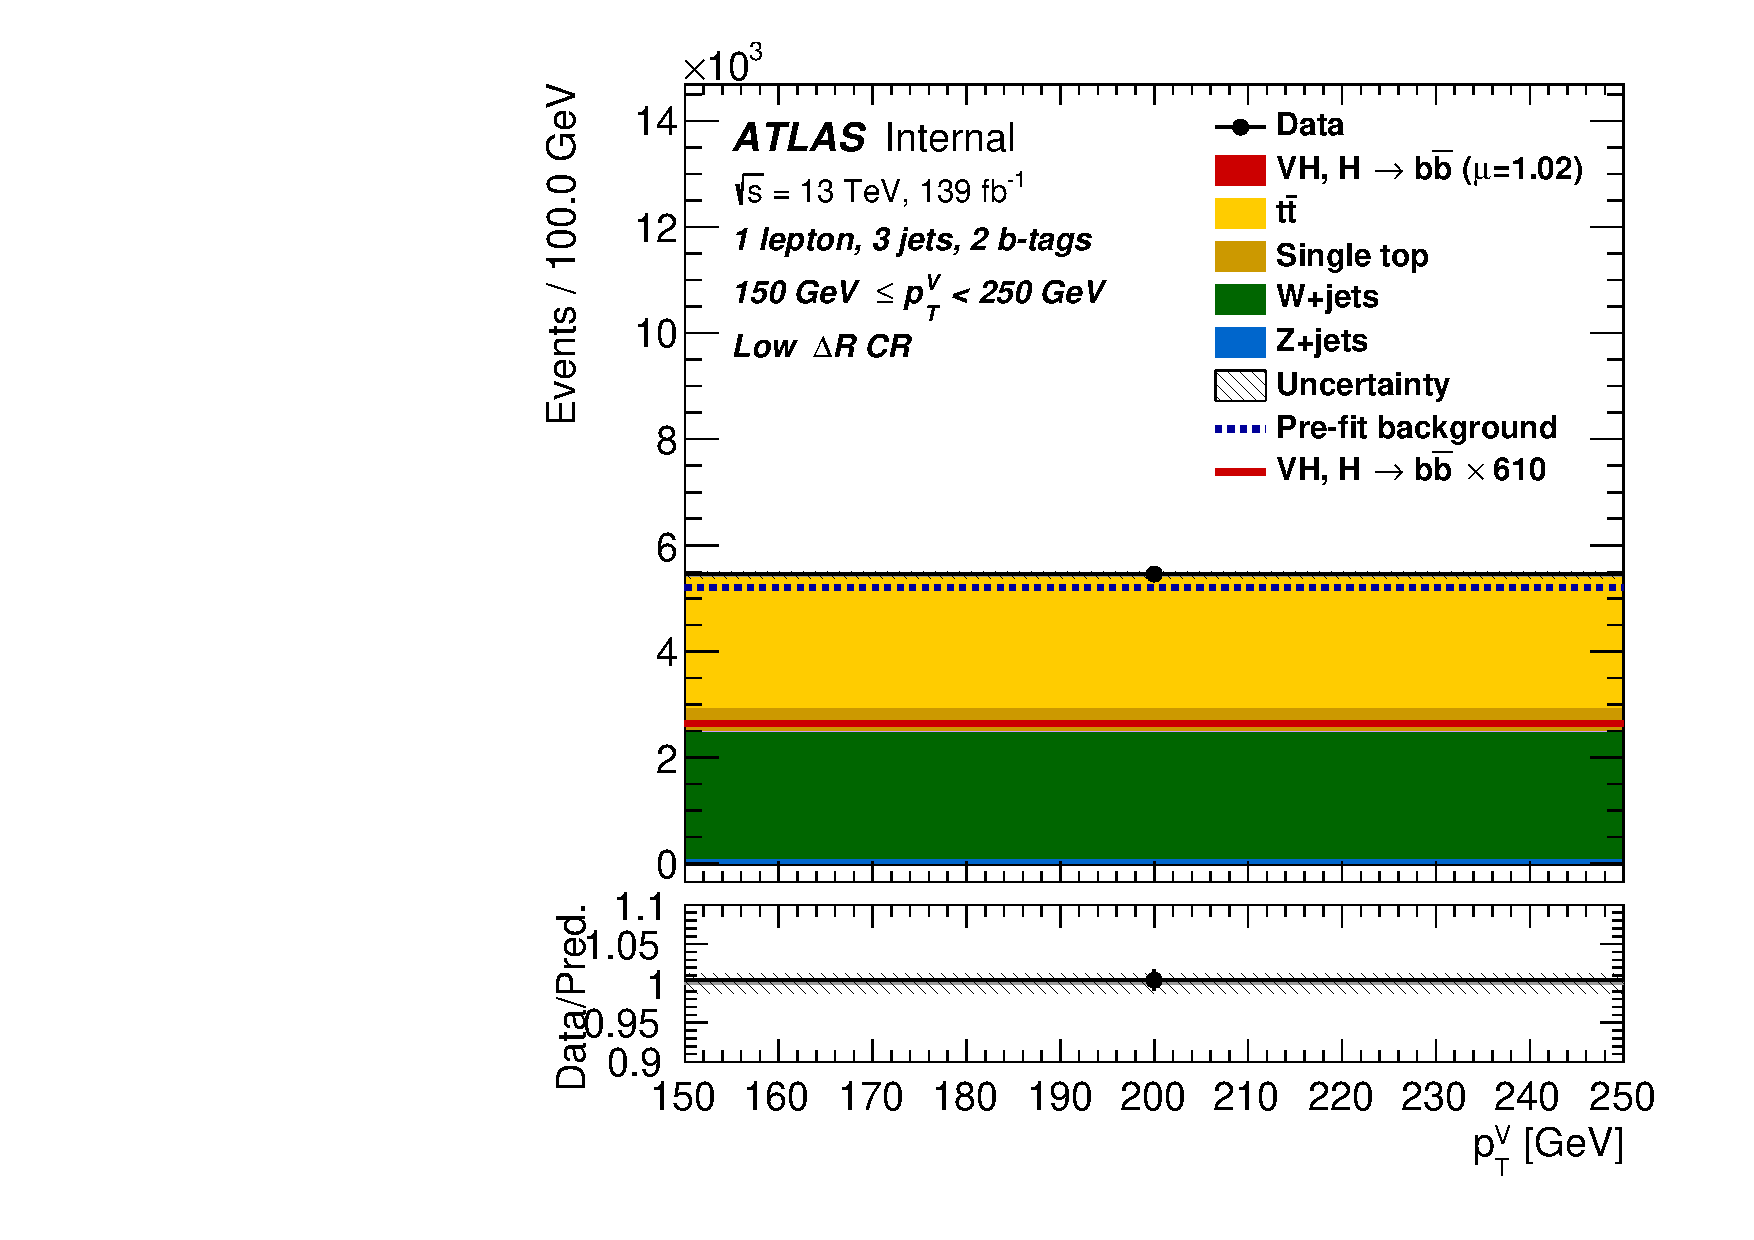
\includegraphics[width=.3\textwidth]{final_fit_mva/postfit/Region_BMax250_BMin150_Y6051_DCRLow_T2_L1_distpTV_J3_GlobalFit_unconditionnal_mu1}%
    & 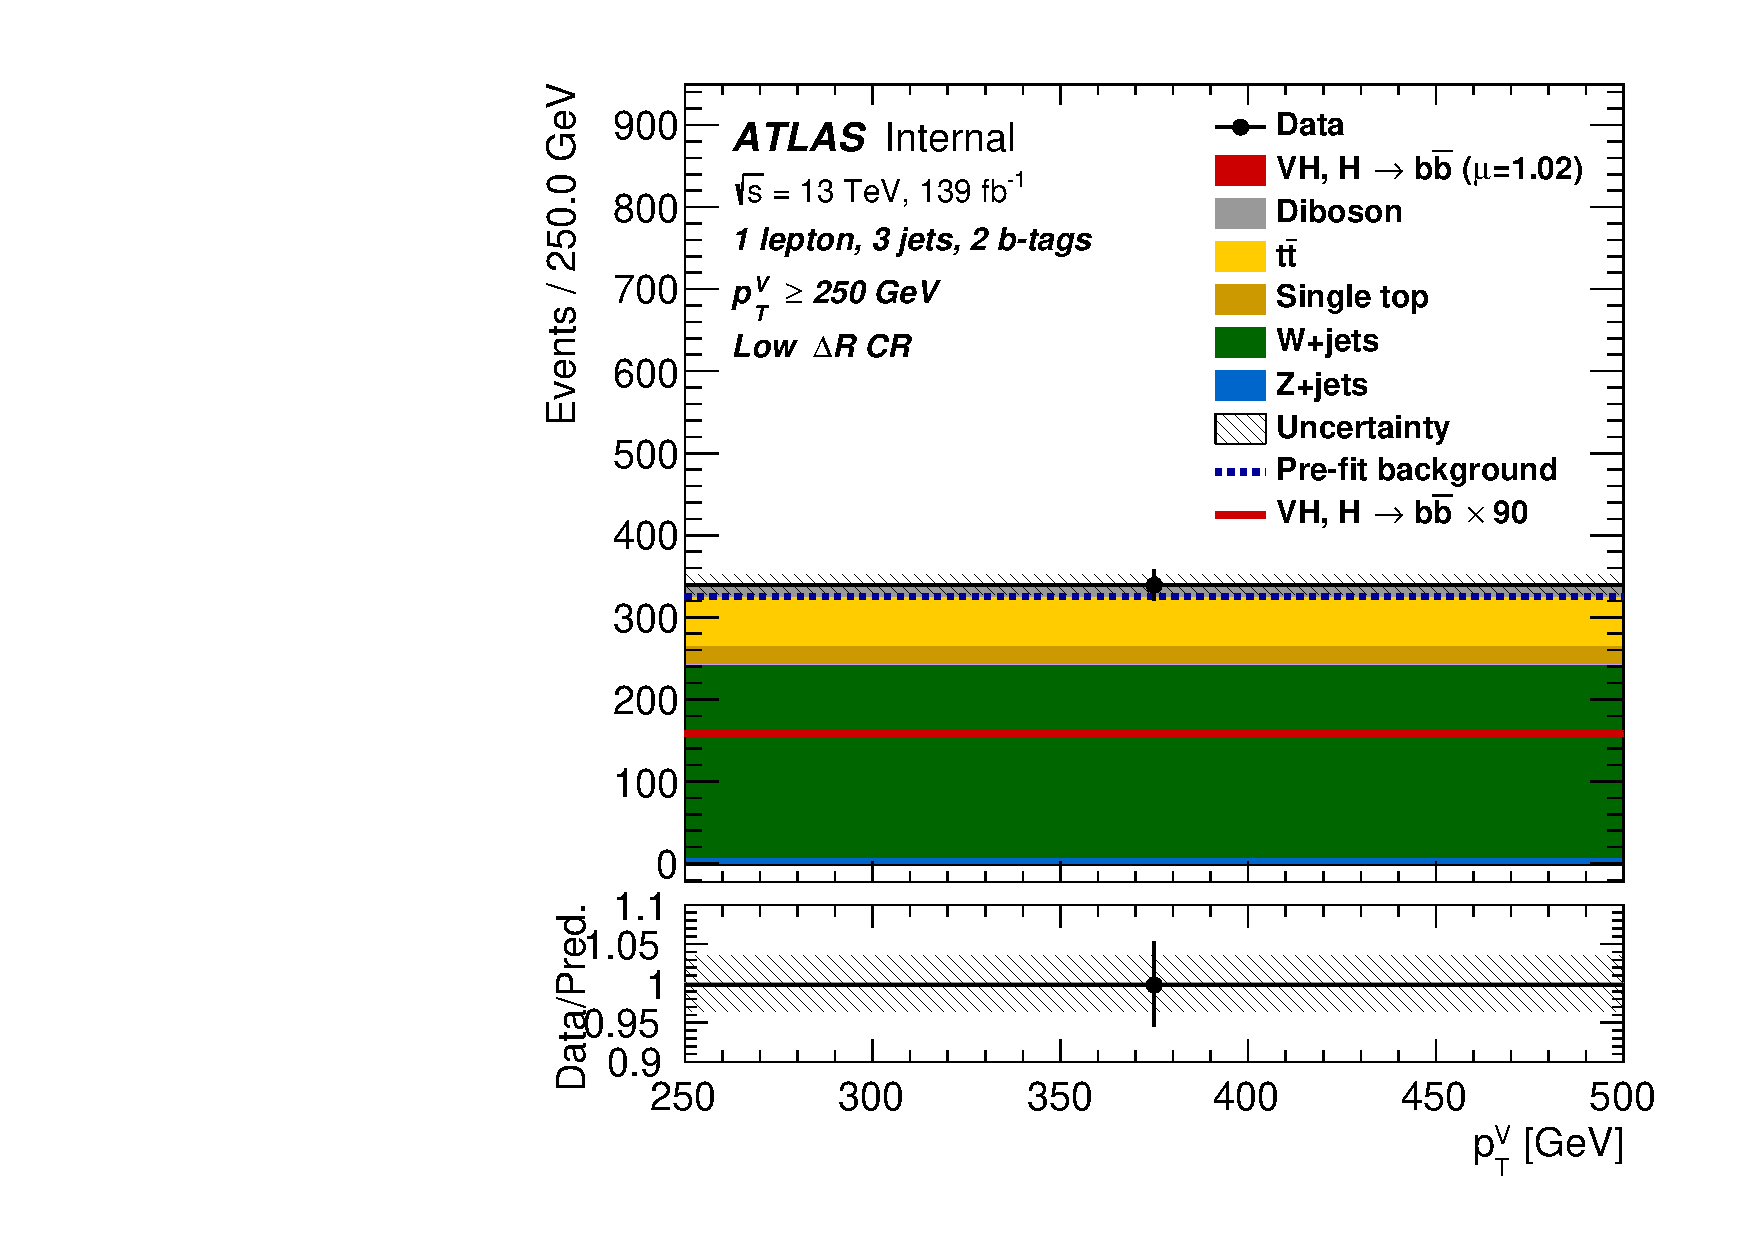
\includegraphics[width=.3\textwidth]{final_fit_mva/postfit/Region_BMin250_Y6051_DCRLow_T2_L1_distpTV_J3_GlobalFit_unconditionnal_mu1} \\
  \end{tabular}
  \caption{Post-fit distributions in the 1 lepton 3 jet channel.}
\end{figure}
\begin{figure}
  \centering
  \begin{tabular}{cc}
    % top row
    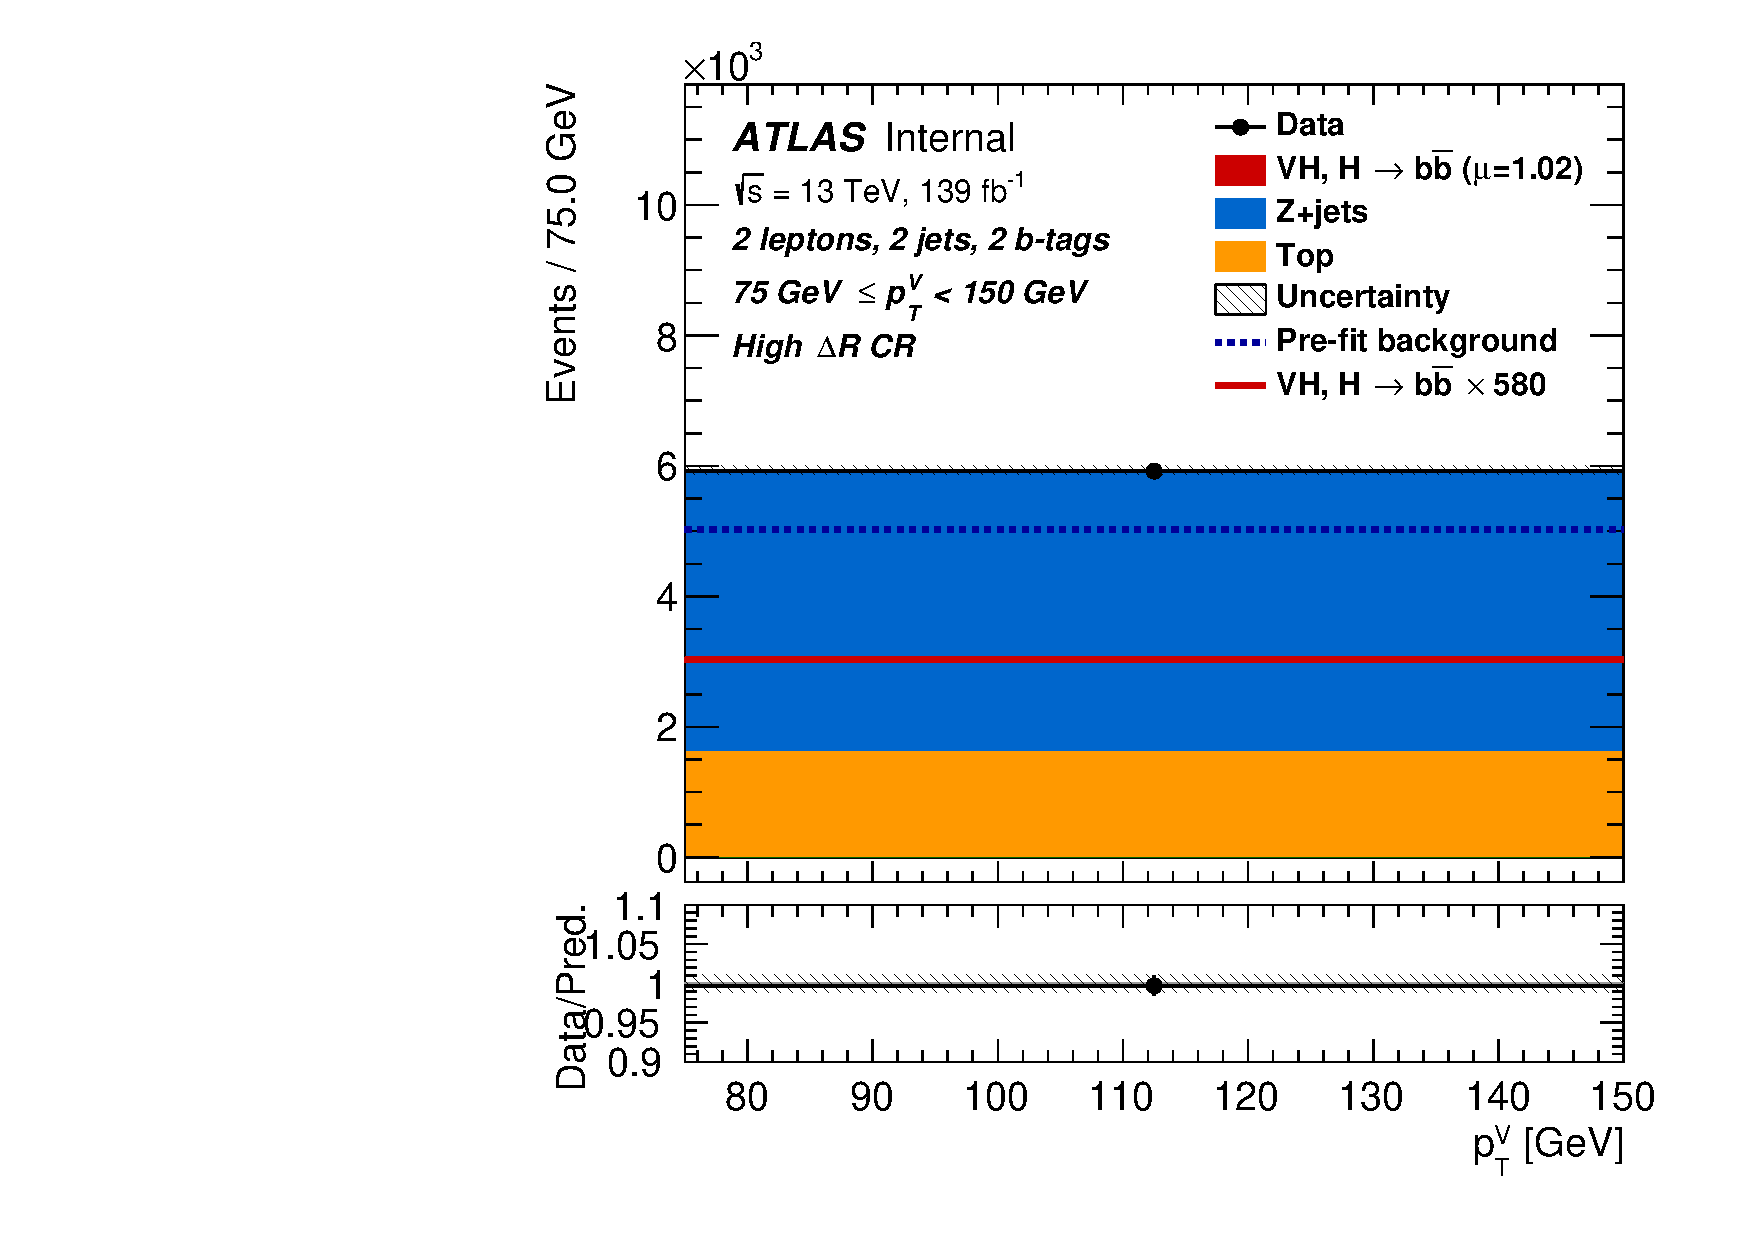
\includegraphics[width=.3\textwidth]{final_fit_mva/postfit/Region_BMax150_BMin75_Y6051_DCRHigh_T2_L2_distpTV_J2_GlobalFit_unconditionnal_mu1}%
    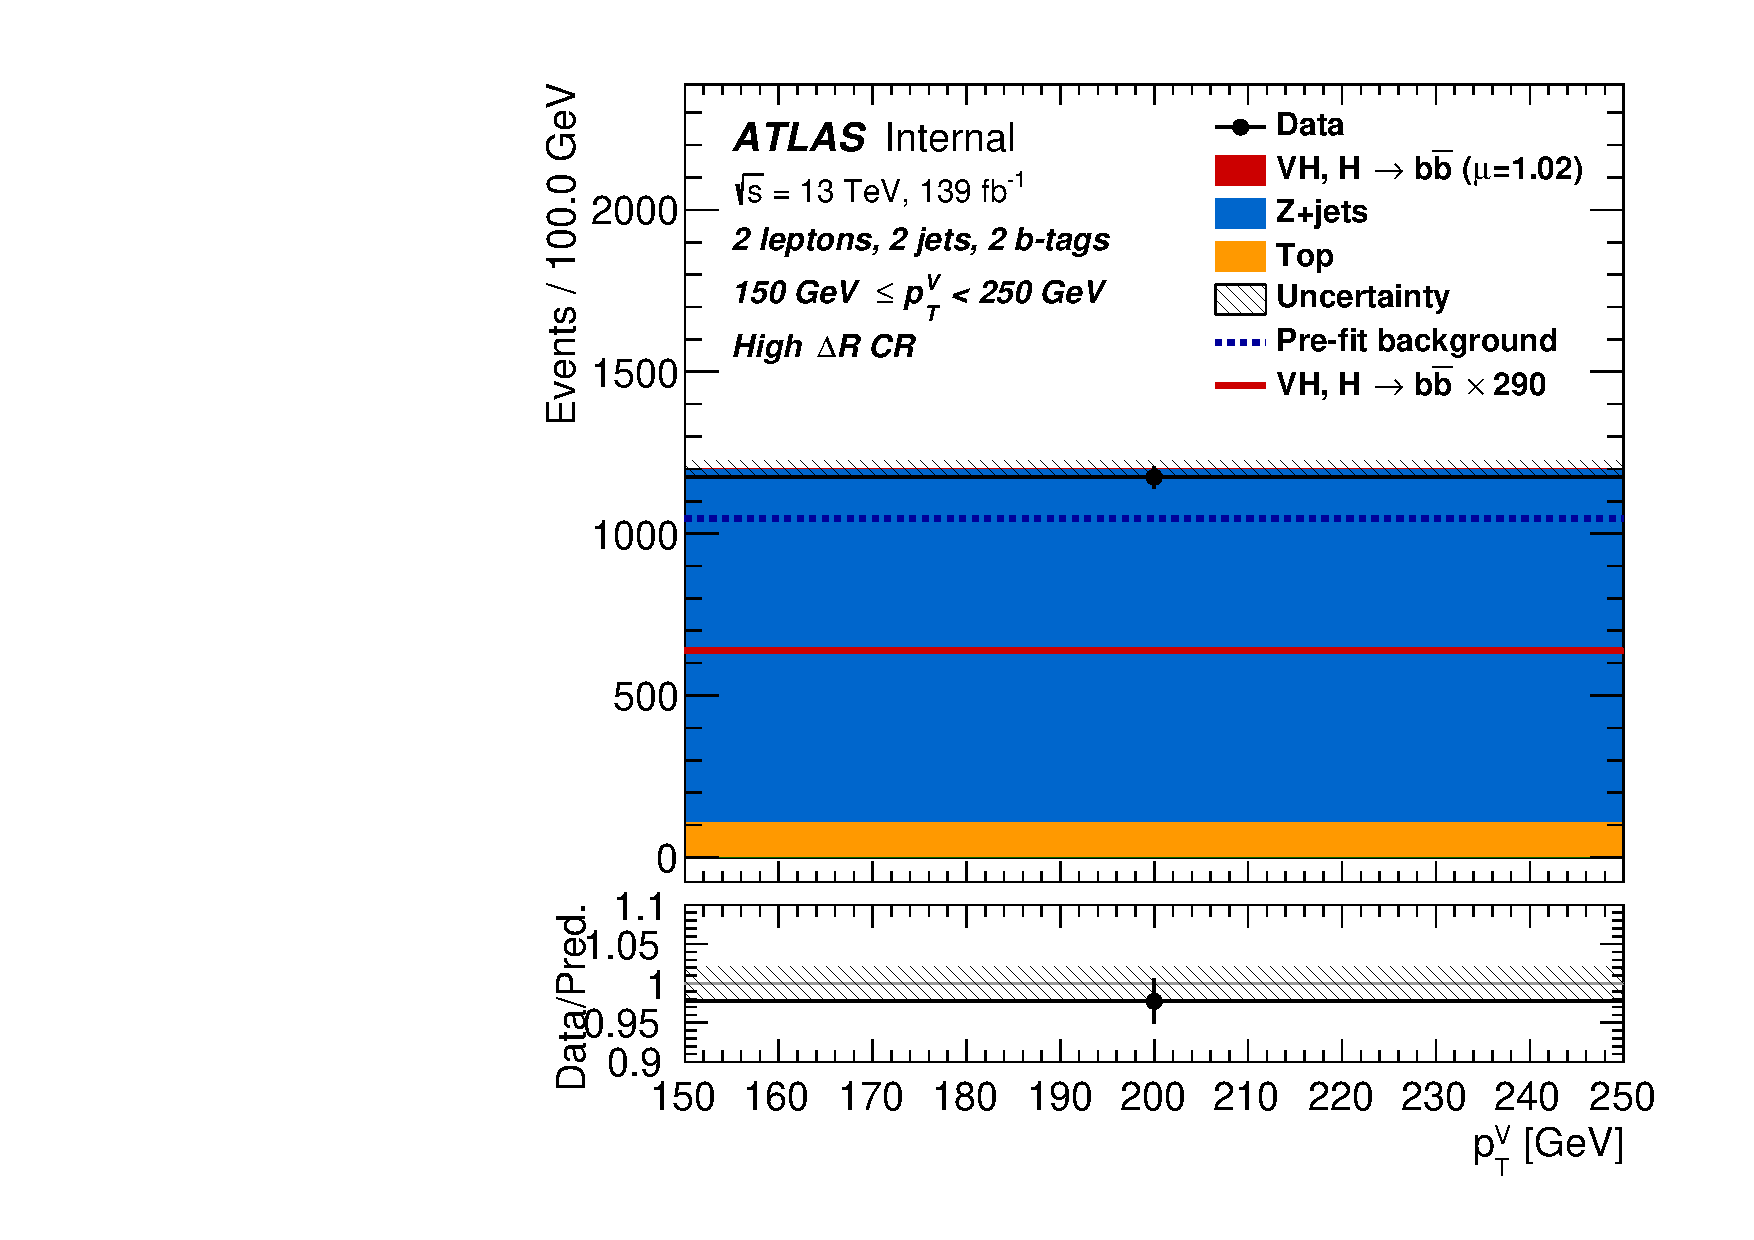
\includegraphics[width=.3\textwidth]{final_fit_mva/postfit/Region_BMax250_BMin150_Y6051_DCRHigh_T2_L2_distpTV_J2_GlobalFit_unconditionnal_mu1}%
    & 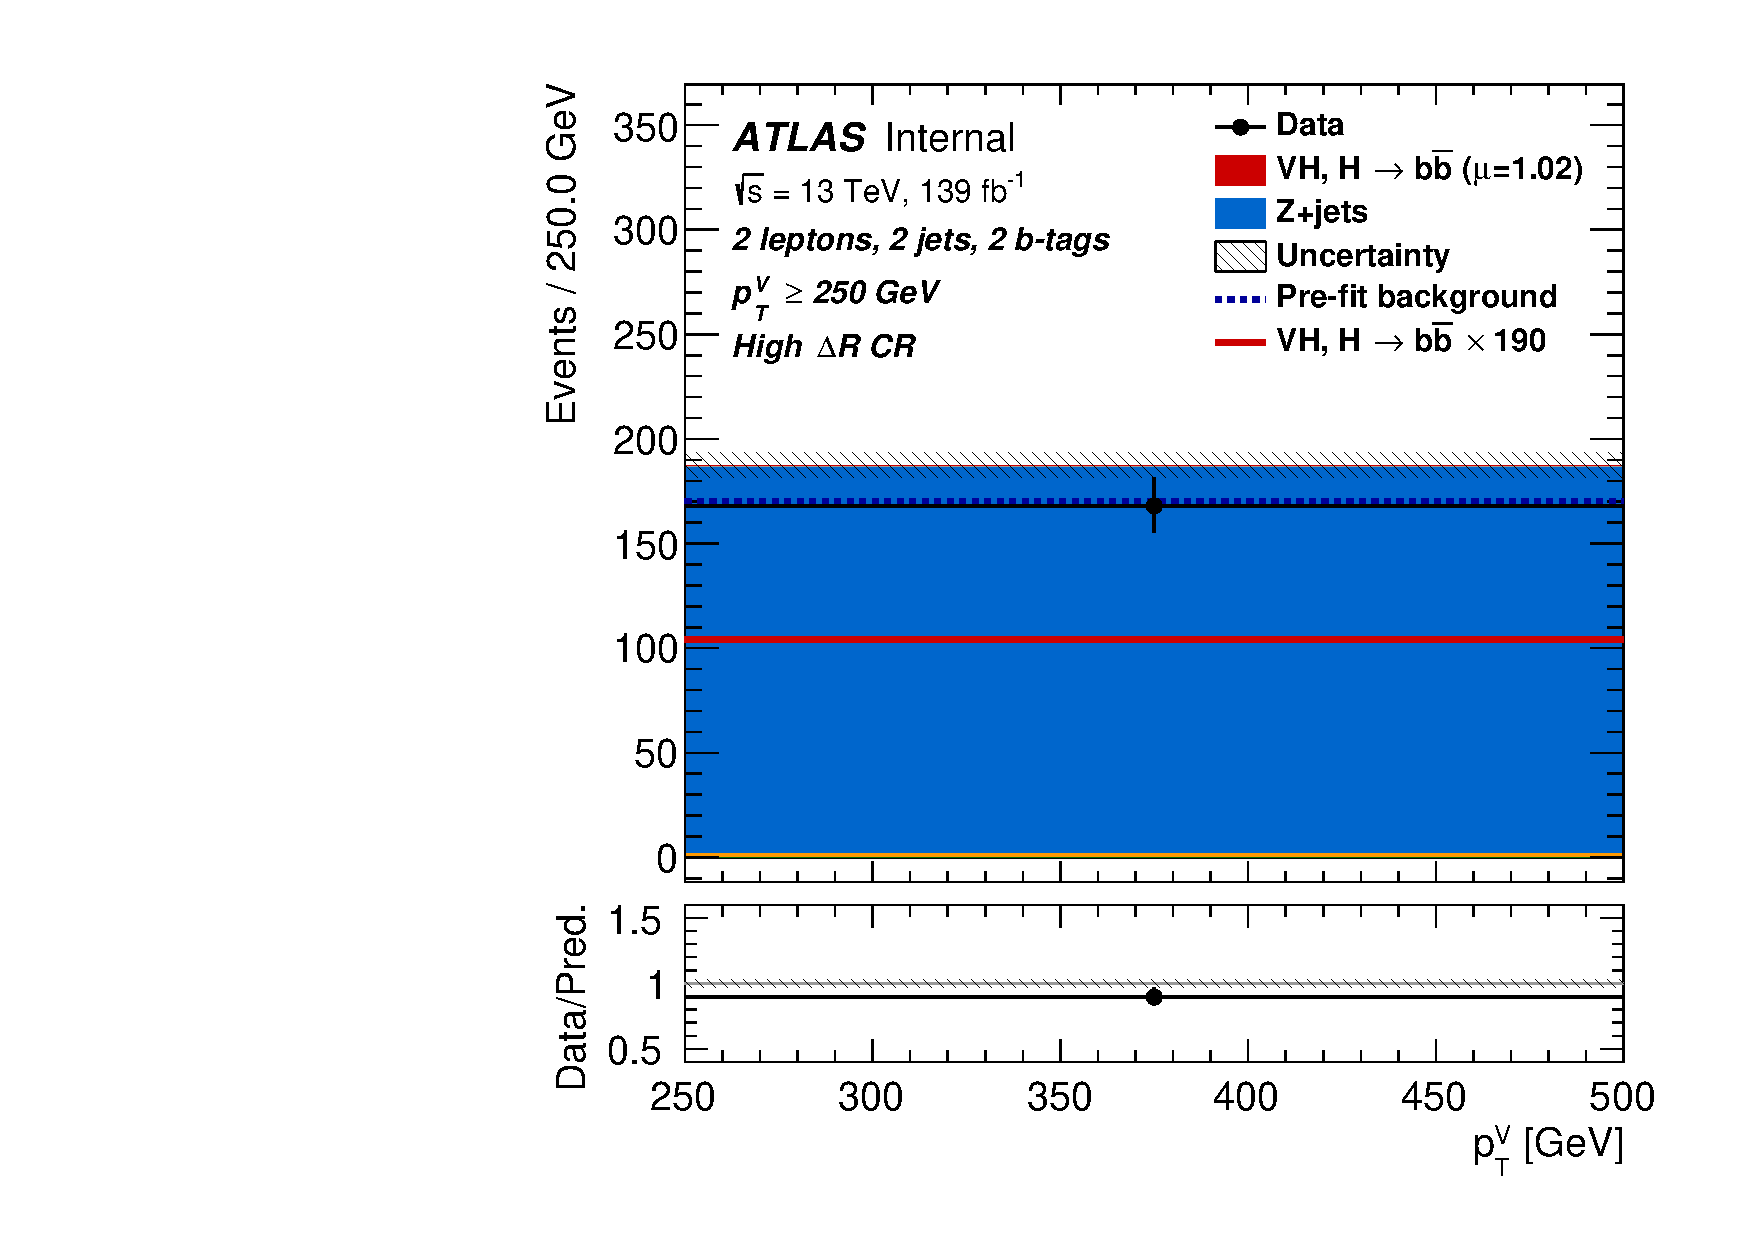
\includegraphics[width=.3\textwidth]{final_fit_mva/postfit/Region_BMin250_Y6051_DCRHigh_T2_L2_distpTV_J2_GlobalFit_unconditionnal_mu1} \\

    % middle row
    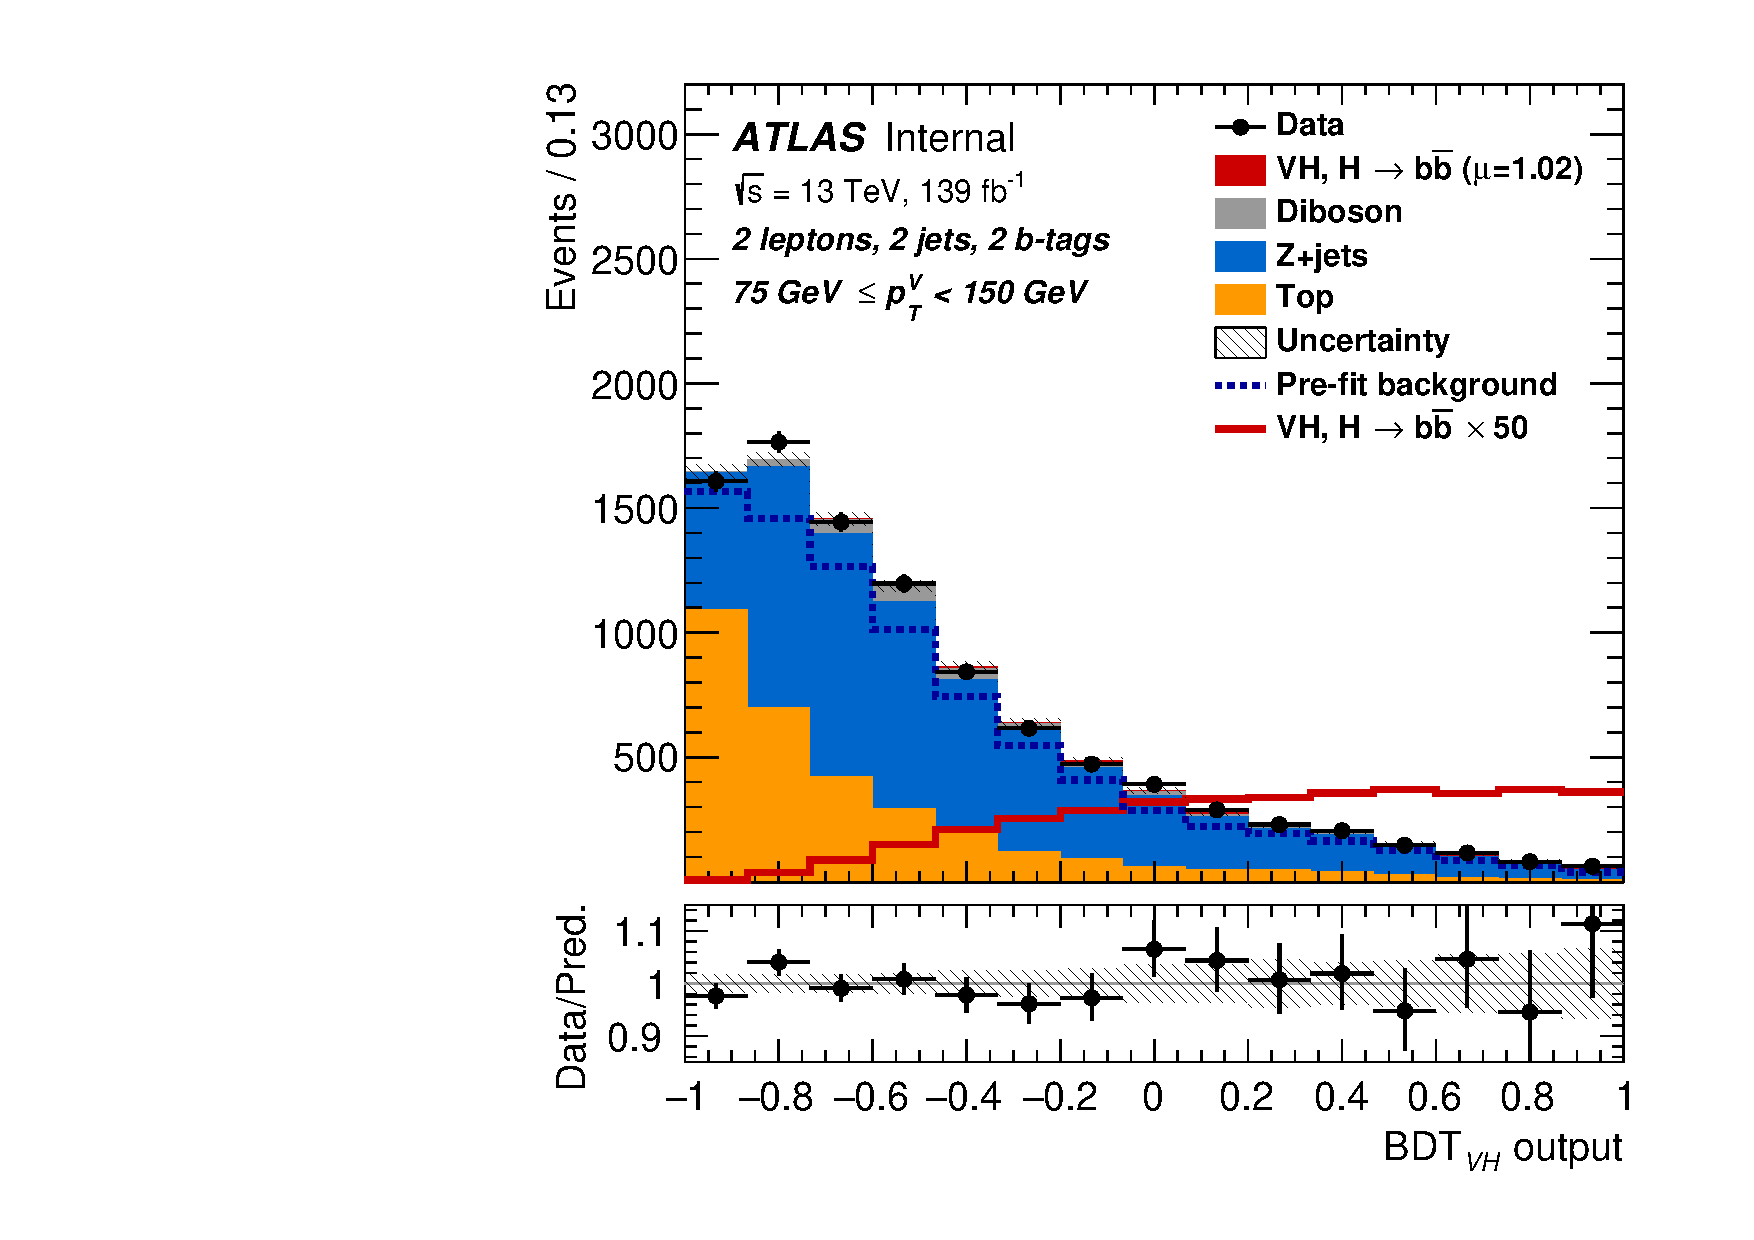
\includegraphics[width=.3\textwidth]{final_fit_mva/postfit/Region_BMax150_BMin75_Y6051_DSR_T2_L2_distmva_J2_GlobalFit_unconditionnal_mu1}%
    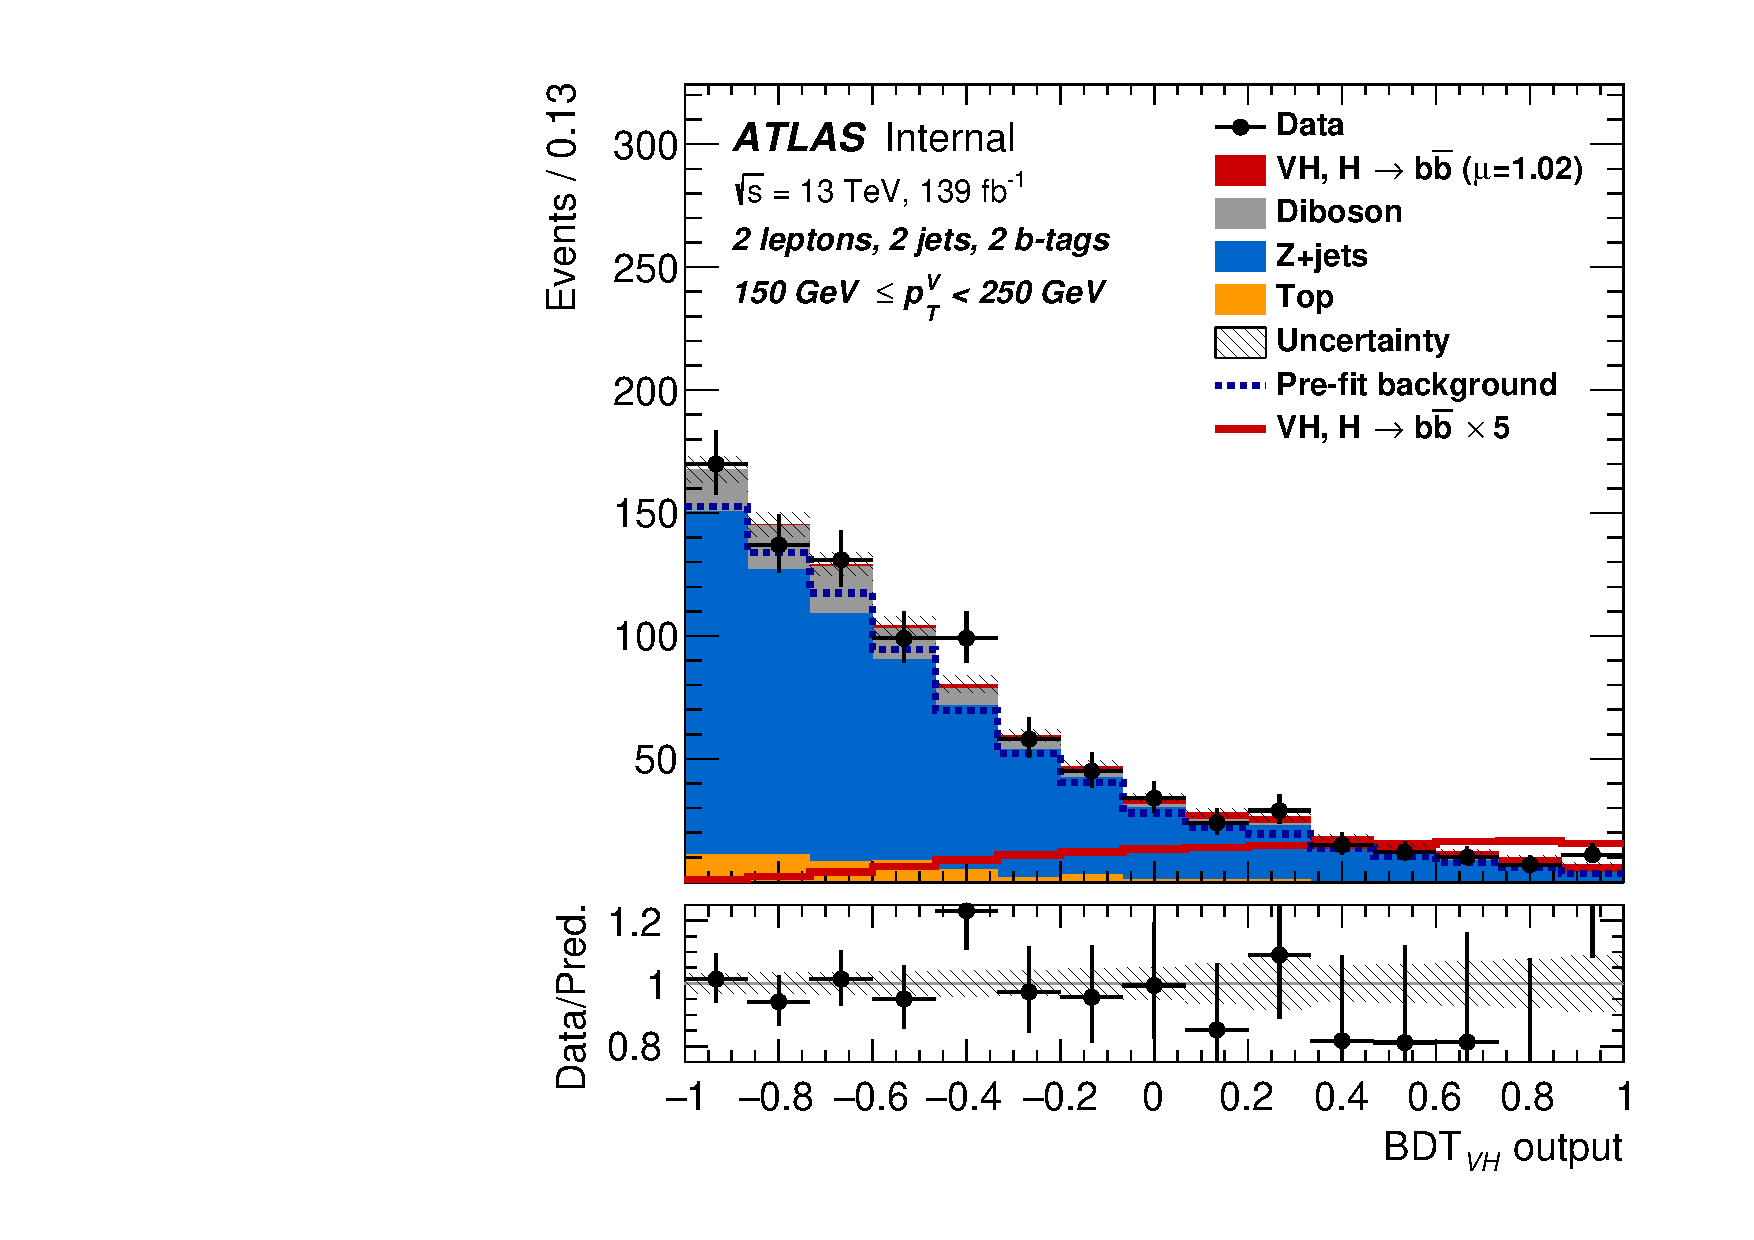
\includegraphics[width=.3\textwidth]{final_fit_mva/postfit/Region_BMax250_BMin150_Y6051_DSR_T2_L2_distmva_J2_GlobalFit_unconditionnal_mu1}%
    & 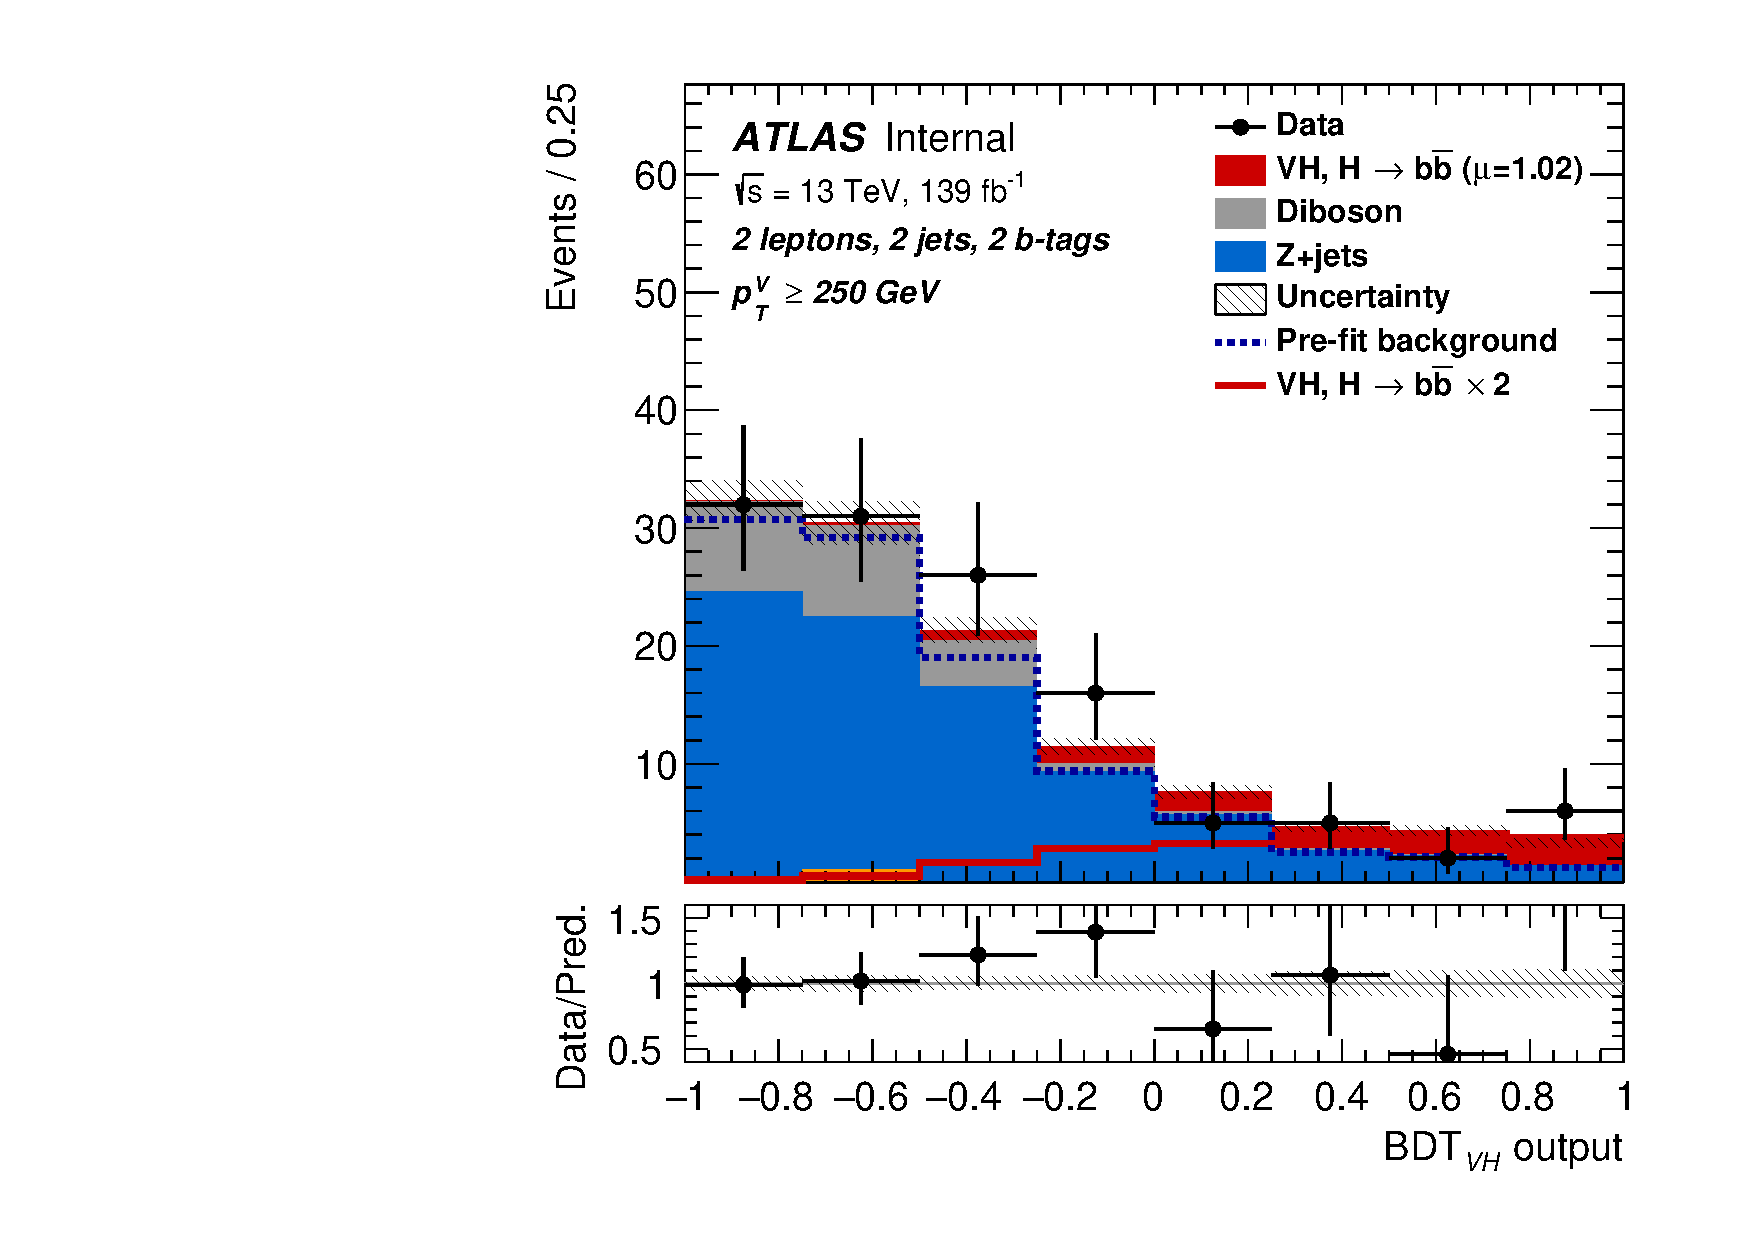
\includegraphics[width=.3\textwidth]{final_fit_mva/postfit/Region_BMin250_Y6051_DSR_T2_L2_distmva_J2_GlobalFit_unconditionnal_mu1} \\

    % bottom row
    \includegraphics[width=.3\textwidth]{final_fit_mva/postfit/Region_BMax150_BMin75_Y6051_DCRLow_T2_L2_distpTV_J2_GlobalFit_unconditionnal_mu1}%
    \includegraphics[width=.3\textwidth]{final_fit_mva/postfit/Region_BMax250_BMin150_Y6051_DCRLow_T2_L2_distpTV_J2_GlobalFit_unconditionnal_mu1}%
    & \includegraphics[width=.3\textwidth]{final_fit_mva/postfit/Region_BMin250_Y6051_DCRLow_T2_L2_distpTV_J2_GlobalFit_unconditionnal_mu1} \\
  \end{tabular}
  \caption{Post-fit distributions in the 2--lepton 2--jet channel.}
\end{figure}
\begin{figure}
  \centering
  \begin{tabular}{cc}
    % top row
    \includegraphics[width=.33\textwidth]{final_fit_mva/postfit/Region_BMax150_BMin75_incJet1_Y6051_DCRHigh_T2_L2_distpTV_J3_GlobalFit_unconditionnal_mu1}%
    \includegraphics[width=.33\textwidth]{final_fit_mva/postfit/Region_BMax250_BMin150_incJet1_Y6051_DCRHigh_T2_L2_distpTV_J3_GlobalFit_unconditionnal_mu1}%
    & \includegraphics[width=.33\textwidth]{final_fit_mva/postfit/Region_BMin250_incJet1_Y6051_DCRHigh_T2_L2_distpTV_J3_GlobalFit_unconditionnal_mu1} \\

    % middle row
    \includegraphics[width=.33\textwidth]{final_fit_mva/postfit/Region_BMax150_BMin75_incJet1_Y6051_DSR_T2_L2_distmva_J3_GlobalFit_unconditionnal_mu1}%
    \includegraphics[width=.33\textwidth]{final_fit_mva/postfit/Region_BMax250_BMin150_incJet1_Y6051_DSR_T2_L2_distmva_J3_GlobalFit_unconditionnal_mu1}%
    & \includegraphics[width=.33\textwidth]{final_fit_mva/postfit/Region_BMin250_incJet1_Y6051_DSR_T2_L2_distmva_J3_GlobalFit_unconditionnal_mu1} \\

    % bottom row
    \includegraphics[width=.33\textwidth]{final_fit_mva/postfit/Region_BMax150_BMin75_incJet1_Y6051_DCRLow_T2_L2_distpTV_J3_GlobalFit_unconditionnal_mu1}%
    \includegraphics[width=.33\textwidth]{final_fit_mva/postfit/Region_BMax250_BMin150_incJet1_Y6051_DCRLow_T2_L2_distpTV_J3_GlobalFit_unconditionnal_mu1}%
    & \includegraphics[width=.33\textwidth]{final_fit_mva/postfit/Region_BMin250_incJet1_Y6051_DCRLow_T2_L2_distpTV_J3_GlobalFit_unconditionnal_mu1} \\
  \end{tabular}
  \caption{Post-fit distributions in the 2--lepton, $\geq$3--jet channel.}
\end{figure}

\clearpage

\section{Signal Strength and STXS Measurements}
%Results will be shown for the \VH\ signal strength measurement, the individual
%\WH\ and \ZH\ signal strength measurements and finally for the STXS measurement.
% Show the signal strength measurements and STXS measurements, everything agrees
% with the standard model so there is not much to state beyond that.

% (+ add in chapter 6 mention the multiple POI version of the fit which yields the
% STXS measurement, briefly describe what this is defining the Njet - NHjet
% procedure to get the STXS bins, i.e. define the fiducial space)
% \begin{figure}[!htbp]
	\centering
	\includegraphics[width=0.7\linewidth]{final_fit_mva/results/Global_SoverB_Y6051_details_pulls.pdf}
  \caption{caption}
  % Data events from the full Run 2 dataset distributed as a function of
  % $\log_{10}(S/B)$ and overlaid on MC predictions after applying the pulls from
  % data.
  \label{fig:sobplot}
\end{figure}

\subsection{\VH\ Signal Strength Measurement}
Table~\ref{tab:sig_channels} shows the expected and observed significances for
the background plus signal hypothesis broken down by analysis channel.
\begin{table}[h]
  \centering
  \begin{tabular}{lrr}
    \toprule
    {\bfseries Channel}  & {\bfseries Expected sig. (cond. data)} & {\bfseries Observed sig.} \\
    \midrule
    0L         & 4.1               &	4.4	    \\
    1L         & 4.1               &	4.0	    \\
    2L         & 4.3               &	4.2	    \\
    0L+1L+2L   & 6.7               &	6.7	    \\
    \bottomrule
  \end{tabular}
  \caption{caption}
  % Expected significances for a single signal strength, or three
  % corresponding to the three leptonic channel (3-$\mu$ fit), in the combined
  % fits of the mva discriminant in the three channels to the cond. data Asimov
  % dataset (data fit with $\mu=1$) and to Run 2 data.
  \label{tab:sig_channels}
\end{table}
The expected significances were determined using an Asimov dataset conditional
on $\mu=1$. All channels are approaching the 5$\sigma$ threshold to claim
discovery and the combined fit is well above the discovery threshold in
agreement with the previous result~\cite{vhbb-obs}. Figure~\ref{fig:channel-mus}
shows the best fit values for the signal strength in each channel and in the
combined paradigm.
\begin{figure}[hb]
	\centering
	\includegraphics[width=0.7\linewidth]{final_fit_mva/results/Plot_mu_0_DecorrPOI_VH.pdf}
  \caption[Best fit values for signal strength broken down by analysis
  channel.]{Best fit values of the signal strength for the 0--, 1-- and 2--
    channels, as well as the combined (Comb.) measurement. Uncertainties are
    broken down into either statistical (Stat.) or systematic (Syst.), with
    those due to scale factors on background processes counted as statistical.}
  \label{fig:channel-mus}
\end{figure}
All measurements are compatible with the standard model prediction of $\mu=1$,
the composition and values of the uncertainties affecting each channel are
similar with the 2--lepton channel being slightly more impacted by statistical
rather than systematic uncertainty.
%\begin{figure}[!htbp]
	\centering
	\includegraphics[width=0.47\linewidth]{final_fit_mva/results/Plot_mu_1_DecorrPOI_J_VH.pdf}
	\includegraphics[width=0.47\linewidth]{final_fit_mva/results/Plot_mu_0_DecorrBMin_VH.pdf}
	\includegraphics[width=0.47\linewidth]{final_fit_mva/results/Plot_mu_15_DecorrPOI_J_L_VH.pdf}
	\includegraphics[width=0.47\linewidth]{final_fit_mva/results/Plot_mu_15_DecorrPOI_BMin_L_VH.pdf}
  \caption{caption}
  % Best values of the signal strength $\mu_{\VH}^{b\bar{b}}$ uncorrelated
  % (multi-$\mu$) between $N($jet$)$ regions (top left), \pTV regions (top right),
  % $N($jet$)$ regions and lepton channels (bottom left), \pTV regions and lepton
  % channels (bottom right) and their combination in the combined unconditional
  % fit to the Run 2 data. The (black) total observed uncertainty is quoted
  % together with its decomposition in the (green) statistical component, and
  % systematic component. In this plot the uncertainty due to background scale
  % factors is included in the statistical component.
\label{fig:channels-mus-uncorr}
\end{figure}
\clearpage
\subsection{\WH\ and \ZH\ Signal Strength Measurements}
Table~\ref{tab:sig_WZH} shows the expected and observed significances for
the background plus signal hypothesis for the \WH\, \ZH\ and \VH measurements.
\begin{table}[ht]
  \centering
  \begin{tabular}{lrr}
    \toprule
    {\bfseries Channel}  & {\bfseries Expected} & {\bfseries Observed} \\
    \midrule
    \WH         & 4.1       &	4.0	\\
    \ZH         & 5.1       &	5.3	    \\
    \VH         & 6.7      	&	6.7	    \\
    \bottomrule
  \end{tabular}
  \caption[Statistical significances of the background plus signal hypothesis
  for \WH\, \ZH\ and \VH\ measurements.]{Statistical significances for the
    background plus signal hypothesis for an Asimov dataset conditional on
    $\mu=1$, called expected and for the data, called observed. All values are
    given standard deviations ($\sigma$s). Significances are shown the \WH\,
    \ZH\ and \VH\ measurements.}
  \label{tab:sig_WZH}
\end{table}
The expected significances were determined using an Asimov dataset conditional
on $\mu=1$. The \WH\ stand alone measurement is approaching the 5$\sigma$
threshold to claim discovery. The \ZH\ stand alone measurement has surpassed the
threshold and the paper associated with this measurement is first proof of
discovery published. Figure~\ref{fig:WZH-mus}
shows the best fit values for the signal strength for each measurement.
\begin{figure}[hb]
	\centering
	\includegraphics[width=0.7\linewidth]{final_fit_mva/results/Plot_mu_1_STXSFitScheme2_VH.pdf}
  \caption{Best fit values of the signal strength for the \WH\, \ZH\ and
    combined (Comb.$\equiv$\VH) processes. Uncertainties are broken down into
    either statistical (Stat.) or systematic (Syst.), with those due to scale
    factors on background processes counted as statistical.}
  \label{fig:WZH-mus}
\end{figure}
All measurements are compatible with the standard model prediction of $\mu=1$,
the composition and values of the uncertainties affecting each channel are very
similar.
\clearpage

\subsection{Simplified Template Cross-section Measurements}
Table~\ref{tab:sig_stxs} shows the expected and observed significances for
the \VHbb\ cross=section measurement in the each STXS bin. All bins show a high
degree of statistical significance. Figure~\ref{fig:5POI-mus} shows the best fit
values for the cross-section times branching ratio ($\sigma \times B$) in each
of the STXS bins.
\begin{table}[h]
  \centering
  \begin{tabular}{lrr}
    \toprule
    {\bfseries Channel}  & {\bfseries Expected sig.} & {\bfseries Observed sig.} \\
    \midrule
    \WH, $150~\GeV<p_{\mathrm{T}}^{\text{miss}}<250~\GeV$     & 2.0               &	1.6	    \\
    \WH, $p_{\mathrm{T}}^{\text{miss}} > 250~\GeV$            & 3.4               &	3.6	    \\
    \ZH, $75~\GeV<p_{\mathrm{T}}^{\text{miss}}<150~\GeV$      & 1.4               &	1.2	    \\
    \ZH, $150~\GeV<p_{\mathrm{T}}^{\text{miss}}<250~\GeV$     & 3.4               &	3.6	    \\
    \ZH, $p_{\mathrm{T}}^{\text{miss}} > 250~\GeV$            & 3.5               &	3.6	    \\
    \VH                                       & 6.7               &	6.7	    \\
    \bottomrule
  \end{tabular}
  \caption{caption}
  % Expected significances for the five STXS parameters compared to a
  % single global one in the combined fits of the mva discriminant in
  % the three channels to the pure cond. data. Asimov data-set and Run
  % 2 data.
  \label{tab:sig_stxs}
\end{table}
All measurements are compatible with the standard model predictions and are
weakly limited by statistical uncertainty. The theoretical uncertainty on the
standard  model prediction is greater for \ZH\ bins than for \WH\ bins.
\begin{figure}[hb]
	\centering
	\includegraphics[width=0.7\linewidth]{final_fit_mva/results/Plot_mu_5POI.pdf}
  \caption{caption}% Best values of the $\sigma\times \text{BR}$ normalized to the SM for
  % $\mathrm{WH}_{150-250}$, $\mathrm{WH}_{\geq 250}$, $\mathrm{ZH}_{75-150}$,
  % $\mathrm{ZH}_{150-250}$, and $\mathrm{ZH}_{\geq 250}$ in the unconditional fit
  % to data. The (black) total observed uncertainty is quoted together with its
  % decomposition in the (green) statistical component, and systematic component.
  % In this plot the uncertainty due to background scale factors is included in
  % the statistical component. The theoretical uncertainty on the SM prediction of
  % the $\sigma\times BR_{i}$ is shown as the gray area around $1$.}
  \label{fig:5POI-mus}
\end{figure}
Figure~\ref{fig:5POI-corr} shows the correlation between each STXS bin, it can
be seen that no two bins are strongly correlated with one another. The lack of
correlation is largely due to the analysis categorisations which serve as
independent measurements of each STXS bin.
\begin{figure}[hb]
  \centering
  \includegraphics[width=0.7\linewidth]{final_fit_mva/results/corr_XS_5POI.pdf}
  \caption{Correlations between the measurements in each of the STXS bins of the
  analysis for the unconditional fit to data.}
  \label{fig:5POI-corr}
\end{figure}
%\begin{table}[hb]
  \setlength{\extrarowheight}{4pt}
  \centering
    \resizebox{\textwidth}{!}{
      \begin{tabular}{llrrrrrr}
        \toprule
         %&  &  &  &  & \multicolumn{3}{c}{\bfseries Syst. unc.} \\
        {\bfseries Process} & {\bfseries $\bm{p_{\mathrm{T}}^V}$ bin} & {\bfseries SM prediction}  & {\bfseries Result} & {\bfseries Stat. unc.} &  {\bfsries Th. sig.} & {\bfseries Th. bkg.}  & {\bfseries Exp.} \\
        \midrule
        $W\rightarrow \ell\nu$ & $150<p_{\text{T}}^{V}<250$~\GeV\         & $24.0 \pm 1.1$ & $19.0^{+12.2}_{-12.0} $ & $^{+7.7}_{-7.7}$ & $^{+1.2}_{-0.5}$ & $^{+5.5}_{-5.5}$  & $^{+6.0}_{-6.0}$ \\
        $W\rightarrow \ell\nu$ & $p_{\text{T}}^{V}>250$~\GeV\             & $7.1 \pm 0.3$ & $7.2^{+2.3}_{-2.1}  $   & $^{+1.9}_{-1.8}$  & $^{+0.4}_{-0.3}$ & $^{+0.8}_{-0.8}$  & $^{+0.7}_{-0.6}$ \\
        $Z\rightarrow \ell\ell / \nu\nu$ & $75<p_{\text{T}}^{V}<150$~\GeV\     & $50.6 \pm 4.1$ & $42.5^{+36.4}_{-35.4}$   & $^{+25.3}_{-25.3}$   &  $^{+6.6}_{-4.6}$ & $^{+17.2}_{-17.2}$ & $^{+20.2}_{-19.2}$ \\
        $Z\rightarrow \ell\ell / \nu\nu$ & $150<p_{\text{T}}^{V}<250$~\GeV\    & $18.8 \pm 2.4$        & $20.5^{+6.4}_{-6.0}$   & $^{+5.1}_{-4.9}$   & $^{+2.3}_{-2.3}$ &  $^{+2.4}_{-2.3}$ & $^{+2.4}_{-2.1}$ \\
        $Z\rightarrow \ell\ell / \nu\nu$ & $p_{\text{T}}^{V}>250$~\GeV\        & $4.9 \pm 0.5$        & $5.4^{+1.7}_{-1.6} $   & $^{+1.5}_{-1.4}$    & $^{+0.6}_{-0.3}$  & $^{+0.5}_{-0.5}$ & $^{+0.3}_{-0.3}$ \\
        \bottomrule
      \end{tabular}
    }
    \caption{caption, ($|y_H|<2.5$, \Hbb), all quantities in fb}
    % Best-fit values and uncertainties for the $VH$,
    % $V\to$~leptons for the cross-section
    % times the $H\to b\bar{b}$ branching ratio, in the reduced STXS scheme.
    % The SM predictions for each region, computed using the inclusive
    % cross-section
    % calculations and the simulated event samples are also shown.
    % The contributions to the total uncertainty in the measurements from
    % statistical (Stat.~unc.) or systematic uncertainties (Syst.~unc.) in
    % the signal modelling (Th.~sig.), background modelling (Th.~bkg.),
    % and in experimental performance (Exp.) are given separately.
    % The total systematic uncertainty, equal to the difference in quadrature between
    % the total uncertainty and the statistical uncertainty, differs from the
    % sum in quadrature of the Th. Sig., Th. Bkg., and Exp. systematic
    % uncertainties due to correlations.
    % All leptonic decays of the $V$ bosons (including those to $\tau$-leptons, $\ell=e,\mu,\tau$) are considered.
    \label{tab:XS3and5POI}
\end{table}
%\begin{figure}[!htbp]
	\centering
	\includegraphics[width=0.7\linewidth]{final_fit_mva/results/Fancy_SM_5POI.pdf}
  \caption{caption}
  % Best values of the $\sigma\times \text{BR}$ for
  % $\mathrm{WH}_{150-250}$, $\mathrm{WH}_{\geq 250}$,
  % $\mathrm{ZH}_{75-150}$, $\mathrm{ZH}_{150-250}$, and
  % $\mathrm{ZH}_{\geq 250}$ in the unconditional fit to data. The
  % (black) total observed uncertainty is quoted together with the
  % (green) statistical component. The observation is compared to the
  % SM prediction, marked with the red lines, and its uncertainty,
  % represented by the red area.
  \label{fig:5POI-fancyMU}
\end{figure}
